%\PassOptionsToPackage{graphicx}
\documentclass[authoryear, review, 12pt]{elsarticle}
\usepackage{amssymb}
\usepackage{amsmath}
\usepackage{amsthm}
\usepackage{psfrag}
\usepackage{comment}
\usepackage[colorlinks]{hyperref}
%\usepackage{cleveref}
\usepackage{mathtools}
\usepackage{makecell}
\mathtoolsset{showonlyrefs=true}
\usepackage{alltt}
\usepackage{booktabs}
\usepackage{longtable}
\usepackage{threeparttablex}
\allowdisplaybreaks
%\modulolinenumbers[5]
\makeatletter
\def\ps@pprintTitle{%
	\let\@oddhead\@empty
	\let\@evenhead\@empty
	\def\@oddfoot{\reset@font\hfil\thepage\hfil}
	\let\@evenfoot\@oddfoot
}
\makeatother
\newcommand{\ra}[1]{\renewcommand{\arraystretch}{#1}}
%\usepackage{amssymb}
% Graphics paths. RELATIVE paths first: they are machine-independent and are the
% reason this list no longer needs a line per username. They resolve against the
% directory pdflatex is RUN from, so they work when compiling inside Data/Draft/
% (the usual case). The absolute paths below are retained only as a fallback for
% compiling from a different working directory or on another machine.
% Do not delete the relative entries when adding a machine.
\graphicspath{
	{"./"}
	{"../Bartek analysis/data/results/"}
	{"../Programs baseline/"}
	{"../"}
	{"../../"}
	{"C:/Users/m.silva/Documents/GitHub/Sunk-entry-costs--endogenous-variety--and-unemployment/Data/Bartek analysis/data/results"}
	{"C:/Users/m.silva/Documents/GitHub/Sunk-entry-costs--endogenous-variety--and-unemployment/Data/Programs baseline"}
	{"C:/Users/m.silva/Documents/GitHub/Sunk-entry-costs--endogenous-variety--and-unemployment"}
	{"C:/Users/msilv/Documents/GitHub/Sunk-entry-costs--endogenous-variety--and-unemployment/Data/Bartek analysis/data/results"}
	{"C:/Users/msilv/Documents/GitHub/Sunk-entry-costs--endogenous-variety--and-unemployment/Data/Programs baseline"}
	{"C:/Users/msilv/Documents/GitHub/Sunk-entry-costs--endogenous-variety--and-unemployment"}
}
\usepackage{tabularx}
\usepackage{comment}
\usepackage{subfig}
\usepackage{graphicx}
%\journal{Journal of Monetary Economics}
%\usepackage{amssymb}
%\usepackage{amsfonts}
\usepackage{geometry}
\usepackage{diagbox}
\usepackage{epstopdf}
\geometry{verbose,tmargin=2cm,bmargin=2cm,lmargin=2.25cm,rmargin=2.25cm} 
\newtheorem{theorem}{Theorem}
\newtheorem{proposition}{Proposition}
\newtheorem{lemma}{Lemma}
\newtheorem{corollary}{Corollary}
\newtheorem{example}{Example}
\newtheorem{remark}{Remark}
\newtheorem{definition}{Definition}
\newtheorem{assumption}{Assumption}
\usepackage{cite}
\usepackage{float}
\newcommand{\bi}{\begin{itemize}}
	\newcommand{\ei}{\end{itemize}}
\newcommand{\pfrac}[2]{\left(\dfrac{#1}{#2}\right)}
\newcommand{\ov}{\overline}
\newcommand{\deriv}[2]{\dfrac{\partial #1}{\partial #2}}
\newcommand{\der}[2]{\frac{\partial #1}{\partial #2}}
\renewcommand{\pfrac}[2]{\left(\frac{#1}{#2}\right)}
\newcommand{\bfrac}[2]{\left[\dfrac{#1}{#2}\right]}
\newcommand{\lfrac}[1]{\frac{#1}{#1-1}}
\newcommand{\curlyfrac}[2]{\left\{\frac{#1}{#2}\right\}}

% Double space footnotes
\newcommand{\note}[1]{\footnote{\begin{doublespace}#1\end{doublespace}}}
% Simplify ll notation
\newcommand{\ptil}{\tilde{p}}
\newcommand{\wtil}{\tilde{w}}
\newcommand{\Ctil}{\tilde{C}}
\newcommand{\Ntil}{\tilde{N}}
\newcommand{\Ltil}{\tilde{L}}
\newcommand{\Stil}{\tilde{S}}
\newcommand{\thetatil}{\tilde{\theta}}
\newcommand{\Ztil}{\tilde{Z}}
\newcommand{\rtil}{\tilde{r}}
\newcommand{\dtil}{\tilde{d}}
\newcommand{\Qtil}{\tilde{Q}}
\newcommand{\mutil}{\tilde{\mu}}
\usepackage{tikz}
\usetikzlibrary{shapes.geometric, arrows, shapes.multipart}
\tikzstyle{arrow} = [very thick, ->, >=stealth, blue!50]
\tikzstyle{startstop} = [ellipse, minimum width=3.5cm, minimum height=1.5cm, text centered, draw=magenta!50, fill=cyan!30]
\usetikzlibrary{arrows}
\definecolor{turquoise}{RGB}{64, 224, 208}

\begin{document}
	\begin{frontmatter}
		\begin{abstract}
		Vacancies comove positively with establishment entry and negatively with exit; states with higher exit rates accumulate larger labor market gaps during recessions. We develop a model of endogenous business formation and exit with labor market frictions to explain these patterns. Monopolistically competitive firms rent labor from specialized recruiters and face exit risk from product obsolescence and stochastic fixed costs. Both business creation and vacancy posting require sunk costs, making them partially predetermined.
		Three results follow. First, the business formation margin affects labor markets through love of variety and the endogenous exit rate. Second, because vacancy posting is a sunk cost, exiting firms simultaneously eliminate jobs and posted vacancies, so destruction shocks shift the Beveridge curve outward--even if vacancies can respond elastically. Third, match separation shocks destroy only filled positions; firms optimally repost, generating positive unemployment-vacancy comovement. Both technology and destruction shocks produce second-round amplification through further exit and reduced product variety.
		We estimate by Bayesian methods targeting conditional moments—impulse responses to a Bartik-identified destruction shock—and unconditional labor market moments. Technology and destruction shocks account for the predominant share of labor market volatility.
		\end{abstract}
		%\begin{keyword}
		%	labor market frictions \sep sunk entry costs \sep estimation \\
		%	\smallskip
		%	\text{JEL Classification: D10; E21; E22; E32; E37}\\
		%\end{keyword}
		
		\title{Role of business formation and exit for unemployment and vacancy dynamics}
		\author[affil1]{Mario Rafael Silva}
		\ead{m.silva@northeastern.edu}
		\author[affil2]{Marshall Urias}
		\address[affil1]{Economics Department, Northeastern University}
		\ead{murias@phbs.pku.edu.cn}
		\address[affil2]{Peking University HSBC Business School}
		\author[affil3]{Zhesheng Qiu}
		\address[affil3]{Hong Kong University of Science and Technology}
		\ead{zheshqiu@ust.hk}
		\fntext[]{}
	\end{frontmatter}
	\section{Introduction}\label{sec:introduction}
	
	Labor market variables do not recover at equal speed, and the 
	disparity does not just depend on the severity of the initial shock. 
	The 2020 recession produced the highest peak unemployment rate of 
	any postwar episode  at 13.0 $\%$, yet labor markets had 
	recovered within two years, accumulating only 26.6 percentage-point 
	quarters of total unemployment excess over twenty quarters from 
	recession onset. The 2008--09 recession generated a smaller peak unemployment rate of 9.9 percent yet produced 76.6 percentage-point 
	quarters of cumulative damage and a recovery stretching across six 
	years. 
	
	The standard Diamond--Mortensen--Pissarides (DMP) framework, 
	in which all separations are identical and firms repost vacancies 
	freely after any job loss, offers no structural account of why two 
	recessions of comparable peak unemployment can generate such 
	different cumulative damage. The reason is that the composition of job loss has no influence on persistence. We argue that a 
	key margin to close the gap is firm destruction --- the permanent elimination 
	of business opportunities and their associated vacancy slots --- 
	which ran at 7.8 percent of base employment in 2008--09 but only 
	2.9 percent in 2020.\footnote{Financial frictions, nominal 
		rigidities, and other margins absent from the benchmark model have 
		each received substantial attention in the literature; we focus on 
		firm destruction and its interaction with endogenous business 
		formation.} When a firm exits, its vacancies vanish permanently and 
	must be rebuilt from scratch at sunk cost.  Recovery requires not 
	merely a rebound in profitability but a costly reconstruction of the 
	vacancy stock, generating a persistent outward shift of the 
	Beveridge curve. By contrast, after a separation at a surviving firm, the position is reposted provided reposting is cheap relative to initial creation, so the aggregate vacancy stock partially self-corrects even while unemployment remains elevated. This  produces a transitory displacement along the Beveridge curve rather than a persistent  outward shift.	
	
	
	\citet{coles_2018} show that extending the DMP model with finitely 
	elastic vacancy creation enables separation shocks to generate a 
	downward-sloping Beveridge curve and, jointly with technology shocks, 
	fit a broad set of labor market moments well. But CK assume a single 
	separation shock, conflating firm destruction and match dissolution 
	into one margin, and separations are entirely exogenous. \citet{gabrovski_2025} build on CK by distinguishing 
	between destruction of a product line $\delta$ and breakdown of a 
	match $s$, and show that, for empirically reasonable values of $\delta$, the model generates mild unemployment-labor productivity comovement under technology shocks alone, and also matches other key 
	labor market moments, including the Beveridge curve. In both 
	frameworks, sunk entry costs make the vacancy stock predetermined: 
	$v_{t-1}$ enters the equilibrium alongside $u_t$, and surviving 
	firms repost vacancies freely following match dissolution, 
	substantially weakening the link between unemployment and 
	contemporaneous productivity.
	
	This paper opens additional channels related to business formation and exit. First, we
	introduce love-of-variety preferences over differentiated product lines, so the mass of
	active product lines $N_t$ becomes a third state variable. Employment and variety feed each
	other, an aggregate demand externality in the sense of \citet{schaal_2019}. A new product
	line raises the welfare-based relative price $\rho(N_t)$, and with it recruiter compensation
	$w^{int}_t=\rho(N_t)z_t/\mu$ and the return to vacancy creation, while greater employment
	expands the resources available for product-line formation.

	We segment the product and labor markets so that a product line employs many workers.
	Employment and the number of product lines therefore do not move one for one, and $u_t$,
	$v_{t-1}$, and $N_t$ are jointly determined without an accounting restriction.\footnote{In \citet{schaal_2019}, each matched
		worker--firm pair produces one variety of an intermediate good,
		so employment and the range of goods fluctuate one-for-one. The
		demand externality therefore operates simultaneously through both
		matching and variety. In our setting, firms employ multiple
		workers per product line, so employment adds output within
		existing varieties while the variety externality operates
		separately through firm entry, governed by the business-formation
		Euler equation.}

	Second, we endogenize firm exit. The realized destruction rate $\delta_{e,t}$ combines an
	exogenous component with a margin that responds to profitability through a
	continuation-cost cutoff, so a recession that lowers profits or raises separations induces
	additional exit. The establishment death rate measured in Section~\ref{sec:empirical} is
	this composite. The same cost distribution supplies the draws that govern which vacated
	positions are reposted, so costly reposting adds no separate distributional assumption.

	These extensions sharpen the asymmetry between $\delta$ and $s$ shocks. A destruction
	shock damages all three state variables at once: it raises $u_t$, depletes the vacancy
	stock, and eliminates product lines that would otherwise sustain vacancy creation. A
	separation shock raises $u_t$, but under costless reposting each separation returns its
	position to the vacancy pool. Section~\ref{sec:mechanism} establishes the asymmetry
	analytically, and Section~\ref{sec:quantitative} assesses how much of the cross-recession
	gap in cumulative labor market damage it accounts for.

	One might ask whether the composition of job loss could be
	studied by building on \citet{gabrovski_2025}, which already
	separates destruction from match dissolution, and leaving
	preferences aside. Our measurement strategy favors the
	business formation block. We identify $\delta$ from
	establishment deaths, so a business opportunity must
	correspond to an establishment, which holds many positions;
	where each opportunity carries a single vacancy, $\delta$
	has to be calibrated to a rate of job destruction instead. A
	finite and endogenous mass of multi-position lines sustained
	by a sunk entry cost requires positive profit per line: free
	entry equates the value of a line to
	$\rho(N_t)f_e/\mu(N_t)$, which vanishes at $\mu=1$, leaving
	no finite mass of lines. Under Dixit--Stiglitz preferences
	the markup and the taste for variety are then the same
	parameter, $\zeta(N)=\mu(N)-1=1/(\varepsilon-1)$. The
	monopolistic competition block is therefore the minimal structure in
	which an establishment-level destruction margin is coherent,
	with the variety externality an implication rather than a
	separate assumption. The structure also makes the weighting
	of the measured exit rate substantive. Because a line holds
	many positions, the employment-weighted and count-weighted
	establishment death rates are distinct objects in the data,
	and it is the former that maps to the mass of positions
	destroyed.
	\subsection{Motivating reduced form evidence}
	% Empirical motivation
	Three empirical facts motivate treating firm destruction as a distinct and quantitatively
	important margin. \textit{First, establishment entry and exit constitute a large and
	cyclically sensitive component of gross job flows}. Table~\ref{tab:jf_t2_ext_2019} extends
	Table 2 of \citet{jaimovich_2008} through 2019Q4 using BLS Business Employment Dynamics
	(BED) data.\footnote{The closings columns use BED \emph{closings}, for comparability with
	\citet{jaimovich_2008}, whose question concerns the number of firms actively competing in a
	period; BED deaths were not published until May 2009. The model's $\delta$ shock is the
	permanent elimination of a product line, so the rest of the paper uses BED \emph{deaths},
	defined in Section~\ref{sec:empirical_instr}.} We stop the sample in 2019Q4. Extending it
	leaves the mean shares almost unchanged but collapses every cyclicality ratio, because 2020
	inflates total job losses without a corresponding rise in permanent exit.

	The entry and exit margins are of comparable size. Opening establishments account for
	$20.0$ percent of gross job gains and closing establishments for $19.5$ percent of gross
	job losses, a share that is stable across industries, from construction ($20.6$ percent) to
	financial activities ($24.7$ percent). Dying establishments, the permanent subset, account
	for $12.0$ percent. The difference, close to two-fifths of the closings margin, is the
	temporary-shutdown component that the $\delta$ instrument must remove. Permanent exit is a
	minority of job destruction but far from a rounding error: about one job loss in eight
	occurs at an establishment that never reopens. The two margins are separately measurable,
	which is what makes the $\delta$-versus-$s$ decomposition empirically tractable.

	All three margins move with the cycle. For total private, the opening flow is the most
	variable, at $0.269$ times the cyclical variation of total job gains under the Hamilton
	filter and $0.275$ under the HP filter. The closing flow moves at $0.239$ times the
	cyclical variation of total job losses, against $0.187$ for deaths ($0.223$ and $0.180$
	under the HP filter). Closings are more cyclical than deaths in every supersector, but the
	gap is wide only in natural resources and mining ($0.205$ against $0.104$), where
	project-based and seasonal establishments suspend operations without exiting. The
	cyclical sensitivity that \citet{jaimovich_2008} document is therefore not an artifact of
	temporary shutdowns. Permanent exit is itself cyclical, which is what the $\delta$ shock
	requires.

	Entry matters too. The damage a destruction shock does is undone only as new
	establishments replace the lines that closed, so the cost and speed of replacement govern
	how long the damage lasts. Openings are procyclical: their correlation with cyclical net
	job change is $0.47$ under the Hamilton filter and $0.31$ under the HP filter, while
	permanent exit runs the other way, at $-0.08$ and $-0.49$.\footnote{Openings and deaths are
	themselves positively correlated ($0.56$ and $0.46$), as two gross flows that share a
	common reallocation component, so we compare each flow with net job change.} Replacement
	is therefore slowest when destruction is heaviest, though the exit side of this comparison
	rests mainly on the HP estimate. Where a business opportunity is a single vacancy slot,
	replacing the opportunity and posting the vacancy are the same act, so the entry margin
	in the table has no separate counterpart.
	%%%%%%%%%%%%%%%%
	\begin{table}[H]
\centering
\small
\caption{Job Gains and Losses from Opening, Closing, and Dying Establishments (\emph{Extended to the COVID cutoff, preferred; estimated on 1992Q3--2019Q4}) \\[2pt]
  {\small\itshape Source: BLS Business Employment Dynamics (BED), quarterly, 12 Bartik supersectors. Replication and extension of Jaimovich \& Floetotto (2008, JME) Table~2.}}
\label{tab:jf_t2_ext_2019}
\begin{tabular}{lccccccccc}
\toprule
 & \multicolumn{3}{c}{Mean share} & \multicolumn{3}{c}{Rel.\ std dev (Ham)} & \multicolumn{3}{c}{Rel.\ std dev (HP)} \\
\cmidrule(lr){2-4}\cmidrule(lr){5-7}\cmidrule(lr){8-10}
Industry & $\bar{g}^O$ & $\bar{g}^C$ & $\bar{g}^D$ & $\sigma^O/\sigma$ & $\sigma^C/\sigma$ & $\sigma^D/\sigma$ & $\sigma^O/\sigma$ & $\sigma^C/\sigma$ & $\sigma^D/\sigma$ \\
\midrule
\midrule
\textbf{Total private} & 0.200 & 0.195 & 0.120 & 0.269 & 0.239 & 0.187 & 0.275 & 0.223 & 0.180 \\
Natural resources \& mining & 0.164 & 0.158 & 0.058 & 0.295 & 0.205 & 0.104 & 0.261 & 0.215 & 0.118 \\
Construction & 0.208 & 0.206 & 0.108 & 0.188 & 0.198 & 0.139 & 0.212 & 0.192 & 0.133 \\
Manufacturing & 0.125 & 0.139 & 0.102 & 0.234 & 0.123 & 0.092 & 0.260 & 0.119 & 0.091 \\
Wholesale trade & 0.204 & 0.227 & 0.155 & 0.260 & 0.249 & 0.206 & 0.296 & 0.250 & 0.213 \\
Retail trade & 0.172 & 0.154 & 0.109 & 0.239 & 0.223 & 0.185 & 0.311 & 0.257 & 0.232 \\
Transportation \& utilities & 0.165 & 0.175 & 0.119 & 0.208 & 0.223 & 0.187 & 0.147 & 0.174 & 0.149 \\
Information & 0.206 & 0.210 & 0.150 & 0.292 & 0.367 & 0.318 & 0.327 & 0.399 & 0.361 \\
Financial activities & 0.235 & 0.247 & 0.170 & 0.352 & 0.387 & 0.331 & 0.481 & 0.455 & 0.410 \\
Prof.~\& business services & 0.205 & 0.212 & 0.127 & 0.288 & 0.239 & 0.215 & 0.290 & 0.246 & 0.193 \\
Education \& health services & 0.202 & 0.213 & 0.128 & 0.341 & 0.336 & 0.275 & 0.455 & 0.429 & 0.313 \\
Leisure \& hospitality & 0.245 & 0.198 & 0.115 & 0.271 & 0.332 & 0.250 & 0.315 & 0.350 & 0.271 \\
Other services & 0.221 & 0.219 & 0.130 & 0.291 & 0.352 & 0.287 & 0.344 & 0.402 & 0.301 \\
\midrule
\multicolumn{10}{p{0.98\linewidth}}{\footnotesize \textit{Notes.} $\bar{g}^O$ ($\bar{g}^C$, $\bar{g}^D$): mean share of gross job gains (losses) from opening (closing, dying) establishments, e.g. $\sum L_D/\sum L$. A death is a closing that reports zero employment for four consecutive quarters, so $\bar{g}^C-\bar{g}^D$ is the temporary-shutdown component. Closings columns replicate Jaimovich \& Floetotto (2008, JME) Table~2, whose sample predates the publication of BED deaths; deaths columns are the permanent-exit margin used in the model. $\sigma^k/\sigma$: relative std dev of the $k$ flow against total flows, raw levels, via the Hamilton (2018) filter ($h{=}8$, $p{=}4$, robust to GFC/Covid outliers) and the HP filter ($\lambda{=}1600$). HP values for total private in the original sample ($\approx 0.33$) closely match Jaimovich \& Floetotto Table~2. Values $<1$: extensive margin less volatile than total flows. $^{*}$ Noisy estimate ($|\text{ratio}|>5$).} \\
\bottomrule
\end{tabular}
\end{table}
	
	
	%%%%%%%%%%%%%%%%%%%%%%%%%%%%%%%%%%%%%%%%%%
	\textit{Second, cumulative establishment exit predicts the severity and persistence of labor market disruption across recessions.} Figure~\ref{fig:recession_scatter_primary} plots the permanence-adjusted establishment exit rate against cumulative unemployment and vacancy gaps across the three post-1992 NBER recessions. The 2008--09 recession generated the largest exit rate (7.8\% of base employment) and the largest cumulative unemployment gap (76.6 pp-quarters), reflecting both a deep trough and a protracted recovery. The 2020 recession, with the smallest exit rate (2.9\%), recovered rapidly on both margins, with a negligible cumulative vacancy shortfall (1.7 pp-quarters). The 2001 recession (exit rate 5.6\%) is the exception on vacancies: its shortfall (25.7 pp-quarters) exceeds the GFC's (18.8), likely reflecting the post-dot-com collapse in investment demand rather than exit. Across the three episodes, larger establishment exit goes with greater and more persistent labor market damage, particularly for unemployment.
	\begin{figure}[H]
		\centering
		\includegraphics[width=0.9\textwidth]{recession_scatter_primary.png}
		\caption{Relationship between cumulative establishment exit rates
			(BED Deaths) during recessions and labor market outcome measures.
			The top row shows quarters from the NBER recession end date until
			unemployment (left) and vacancy (right) rates recover 50\% of the
			trough gap. The bottom row shows the cumulative unemployment gap
			(CUG, left) and cumulative vacancy shortfall (CVS, right), defined
			as the sum of positive deviations from the pre-recession baseline
			over $H=20$ quarters from recession onset. Exit rates are constructed
			from BLS Business Employment Dynamics (BED) establishment deaths
			(establishments absent for four or more consecutive quarters),
			normalized by 2006 base-year employment.}
		\label{fig:recession_scatter_primary}
	\end{figure}
	
	\textit{Third, states with structurally higher establishment exit rates 
	accumulate larger labor market gaps during recessions.} 
	Figure~\ref{fig:state_scatter} plots each state's full-sample 
	average Bartik-weighted establishment exit rate against its 
	cumulative unemployment gap (CUG) and cumulative vacancy shortfall 
	(CVS), both summed over 20 quarters from recession onset and 
	averaged across the 2001, 2007--09, and 2020 recessions. The 
	labor-force-weighted cross-sectional correlations are 0.65 (CUG) 
	and 0.28 (CVS): states with structurally higher exit propensity 
	accumulate substantially more total unemployment damage during 
	downturns, with the vacancy pattern weaker but directionally 
	consistent. The stronger CUG correlation is itself informative --- 
	it suggests that exit intensity shapes the \emph{duration} of 
	labor market distress more than the \emph{depth} of the vacancy 
	shortfall, consistent with the model's prediction that firm 
	destruction generates persistent Beveridge curve dislocations 
	rather than transitory displacements.\footnote{The weaker CVS 
		correlation is also consistent with the model: the vacancy stock 
		partially self-corrects through reposting by surviving firms, 
		attenuating the cross-state vacancy signal relative to the 
		unemployment signal.} However, the cross-sectional pattern 
	conflates structural differences in industrial composition with 
	the causal effect of exit shocks: high-exit states may differ 
	from low-exit states along dimensions --- industry mix, 
	institutional environment, average firm age --- that independently 
	predict labor market performance. To isolate causal transmission, 
	we construct Bartik shift-share instruments 
	that exploit within-state variation in exit exposure driven by 
	national industry-level closing rates rather than local conditions, 
	building separate instruments for $\delta$ from BED establishment
	deaths and for $s$ from JOLTS layoff and discharge rates. We 
	then estimate local projection impulse response functions to 
	externally identify the dynamic transmission of each shock to 
	state-level unemployment and vacancies, providing a 
	quasi-experimental foundation for the structural parameters prior 
	to Bayesian estimation.
	\begin{figure}[H]
		\centering
		\includegraphics[width=0.92\textwidth]{state_scatter_primary.png}
		\caption{Cross-state relationship between average establishment exit rates
			and cumulative recession labor market damage. Each point is one of the 50
			U.S.\ states; bubble size is proportional to average labor force.
			The horizontal axis is the full-sample time average of the state-level
			Bartik-weighted establishment exit rate ($\bar{g}^\delta_i$,
			1992Q3--2021Q4), constructed from BLS Business Employment Dynamics (BED)
			data using 2006 base-year employment shares.
			The left panel shows the cumulative unemployment gap (CUG): the
			sum of quarterly deviations of the unemployment rate above its
			pre-recession average over $H=20$ quarters from recession onset,
			in percentage-point-quarters. The right panel shows the analogous
			cumulative vacancy shortfall (CVS) for the vacancy rate.
			Both outcomes are averaged across the three post-1992 NBER recessions
			(2001, 2007--2009, 2020), weighted by state labor force at recession onset.
			The regression line is estimated by WLS with state labor force weights;
			$r_w$ denotes the labor-force-weighted correlation.}
		\label{fig:state_scatter}
	\end{figure}
	
	%
	Following \citet{goldsmith_2020}, we bring quasi-experimental discipline to the $\delta$ transmission 
	channel using Bartik shift-share instruments constructed from 
	BED establishment deaths --- the subset of closings absent from
	the UI payroll base for four or more consecutive quarters,
	aligning the instrument directly with the model's concept of
	irreversible product-line destruction. The instrument weights
	leave-one-out national industry-level death rates by each state's 
	base-year (2006) industry employment shares. The identifying 
	variation is geographic: a state with high pre-recession exposure 
	to industries experiencing national waves of establishment closings 
	--- manufacturing in 2008--09, for instance --- faces a large exit 
	shock driven by national industry conditions rather than local 
	demand, and can be compared to low-exposure states in the same 
	quarter to isolate the causal labor market effect of firm 
	destruction. The instrument is residualized on aggregate 
	productivity growth to address cross-instrument correlation arising 
	mechanically during aggregate downturns. 
	
	We estimate panel local projections \citep{jorda_2005} with state and time fixed effects, 
	standard errors clustered at the state level, and outcomes capped 
	at 2019Q4 to exclude the Covid episode. A one-standard-deviation rise in the $\delta$
	instrument raises unemployment and lowers vacancies persistently. The unemployment rate
	rises by $0.22$ percentage points on impact, significant from $h=0$, and keeps rising,
	to about $1.71$ points after four to five years. The vacancy rate falls, significantly
	from $h=2$, to $-0.58$ points at $h=18$. Both patterns are consistent with the model's prediction that firm
	destruction generates a persistent outward shift of the Beveridge 
	curve rather than a transitory displacement along it.\footnote{The $\delta$ unemployment response concentrates almost entirely in states experiencing tight 
		financial conditions: at average financial conditions the point 
		estimate is near zero and insignificant at all horizons beyond 
		$h=0$. This state-dependence in the unemployment channel, absent 
		from the baseline model, is consistent with financial 
		amplification of firm destruction and is left for future work; 
		the vacancy channel, which enters the structural estimation as a 
		moment condition, does not exhibit the same state-dependence.}
	
	We estimate the model by Bayesian simulated method of moments with two sets of moments.
	The first follows \citet{coles_2018}: unconditional moments of unemployment, vacancies,
	labor productivity, and the job-finding and separation rates, augmented with the mean and
	relative volatility of the establishment death rate, which disciplines the destruction
	process directly rather than inferring it from labor market outcomes. The second is the
	$\delta\to u$ and $\delta\to v$ responses from the Bartik local projections, matched with
	inverse-variance weights. The unconditional moments pin down the destruction process and
	the steady state. The conditional moments discipline how costly and slow vacancy
	replacement is after a destruction shock, which the vacancy creation cost parameters $\xi$
	and $x_m$ govern. Section~\ref{sec:quantitative} reports the results, together with a comparison
	with the clone-replacement benchmark of Section~\ref{sec:equilibrium}, which abstracts
	from variety and endogenous exit.
	
	This paper contributes to four strands of literature. The first 
	is search-and-matching models with finitely elastic vacancy 
	creation, where our model builds most directly on 
	\citet{coles_2018} and \citet{gabrovski_2025}; \citet{broer_2025} 
	independently combine finitely elastic vacancy creation with 
	endogenous separation but abstract from product variety and the 
	separate destruction margin. The second is endogenous product 
	variety and firm dynamics in business cycles, where we build on 
	\citet{bilbiie_2012} and depart from the one-firm-one-worker 
	structure of \citet{shao_2013}; \citet{colciago_2021} combine 
	endogenous entry with labor market frictions in a related 
	framework but maintain infinitely elastic vacancy creation and 
	abstract from the destruction margin. The third is Bartik 
	shift-share identification in local labor markets 
	\citep{goldsmith_2020, nakamura_2014}, discussed alongside the 
	instrument construction in Section~\ref{sec:empirical}. The 
	fourth is Bayesian structural estimation of search models, 
	extending the simulated method of moments approach of 
	\citet{coles_2018} to incorporate impulse response matching as 
	an additional set of moment conditions \citep{christiano_2016}.

	Sections~\ref{sec:environment} and~\ref{sec:equilibrium} present the model, its
	equilibrium, and the analytical results on the $\delta$--$s$ asymmetry.
	Section~\ref{sec:empirical} presents the Bartik local projections,
	Section~\ref{sec:quantitative} the quantitative analysis, and
	Section~\ref{sec:conclusion} concludes.
	
	
	%%%%%%%%%%%%%%%%%%%%%%%%%%%%%%%%%%%%%%%%%%
	\section{Environment}\label{sec:environment}
	%%%%%%%%%%%%%%%%%%%%%%%%%%%%%%%%%%%%%%%%%%
	
	Time is discrete and infinite. The economy is populated by 
	households, intermediaries (recruiters), and retailers. Households 
	and recruiters each have unit mass. There is an endogenous mass of retailers, each supplying one product line. A household consists 
	of a large family of workers who are either employed or unemployed, 
	as in \citet{merz_1995}. Employed members supply one unit of labor 
	inelastically. The household consumes and purchases equity. A unit 
	measure of recruiters can each create one vacancy at a time, at a 
	sunk cost drawn from a known distribution, with each vacancy 
	specialized to a single product line. Retailers rent labor services
	from matched recruiters and produce the specialized variety.

	\paragraph{The model at a glance}
	Two blocks interact. The \emph{business formation block}, in which households invest in new
	product lines and retailers decide whether to continue, determines the mass of product
	lines $N_t$. The \emph{labor market block}, in which recruiters create, fill, and reactivate
	vacancies and bargain over wages, determines unemployment $u_t$, vacancies $v_t$, and
	tightness $\theta_t$. Three objects link them. Recruiter compensation
	$w_t^{int}=\rho(N_t)z_t/\mu(N_t)$ carries product variety into the value of a match. The
	survival probability of a product line, $(1-\delta_t)F(\chi_{t+1}^c)$, applies to every
	position attached to the line, so exit destroys jobs and vacancies together. Employment
	and vacancy costs $X_t$ in turn set output and hence the return to entry. Three shocks
	drive the economy: technology $z_t$; product destruction $\delta_t$, which removes product
	lines together with their positions; and match separation $s_t$, which dissolves a match
	but leaves its position open to reactivation. Section~\ref{sec:equilibrium} derives each block,
	and Proposition~\ref{prop:independence} states when the two separate. \ref{app:notation}
	collects the notation.
	
	Each period a number $m(u_t,v_t)$ of recruiter--worker pairs form, 
	given unemployment $u_t$ and vacancies $v_t$. We adopt the 
	Cobb-Douglas matching function $m(u,v)=Au^{\eta_L}v^{1-\eta_L}$, 
	where $\eta_L$ is the elasticity of matches with respect to 
	unemployment \citep{petrongolo_2001}. Constant returns to scale 
	implies that the job-finding rate $f(\theta)=A\theta^{1-\eta_L}$ 
	and the vacancy-filling rate $q(\theta)=A\theta^{-\eta_L}$ depend 
	only on market tightness $\theta\equiv v/u$.
	\subsection{Preferences}
	
	We develop the model with general homothetic preferences as in 
	\citet{bilbiie_2012}, then apply specific functional forms in the 
	quantitative analysis. The household consumes a basket $c_t$, a 
	homothetic aggregate over a continuum of goods $\Omega$. The 
	welfare-based price index $P_t$ takes only individual prices as 
	arguments, and demand for variety $j$ satisfies
	\begin{align}\label{eq:demand}
		c_{jt}=c_t\partial P_t/\partial p_{jt}.
	\end{align}
	The symmetric price elasticity of demand is in general a function 
	of the measure $N_t$ of goods:
		$\varepsilon(N_t)=-\der{\log c_{j}}{\log p_{j}}$.
	The welfare gain from an additional product variety is captured by 
	the relative price and its elasticity:
	\begin{align}\label{eq:relative_price}
		\rho_{j}=\rho(N)\equiv \frac{p_{j}}{P},\quad 
		\zeta(N)=\frac{\rho'(N)}{\rho(N)}N.
	\end{align}
	The relative price rises with variety: with more products available 
	at the same nominal price, the welfare-based cost of living falls, 
	so $\rho$ increases. Equivalently, spreading consumption across 
	more goods benefits the household. The two statistics 
	$\varepsilon(N_t)$ and $\rho(N_t)$ completely characterize 
	symmetric homothetic preferences in the model.
	
	Under standard Dixit--Stiglitz preferences (DS-CES), $\varepsilon$ 
	measures both the taste for diversity and the elasticity of 
	substitution, so both the markup and the variety benefit are 
	independent of the number of producers: 
	$\zeta(N)=\mu(N)-1=1/(\varepsilon-1)$. Generalized CES, following
	\citet{benassy_1996}, disentangles the taste for variety $\zeta$ from the elasticity of
	substitution $\varepsilon$. \ref{app:preferences} gives the indices, markup, relative
	price, and benefit of variety under both, and under the translog preferences of
	\citet{feenstra_2003}.
	
	\subsection{Laws of motion for firms, unemployment, and vacancies}
	
	A product line survives into  the production phase of period $t$ if it was not destroyed exogenously at the end of $t-1$ (probability 
	$1-\delta_{t-1}$) \emph{and} its owner draws a continuation cost below the equilibrium cutoff $\chi_t^c$ at the start of $t$.
	Continuation costs, in units of the consumption basket, are drawn from a mixture of a
	mass point at zero, with probability $1-p_0$, and a bounded power law:
	\begin{align}\label{eq:F_chi}
		F(\chi) = (1-p_0) + p_0\left(\frac{\chi}{\chi_m}
		\right)^\psi,
		\quad \chi\in[0,\,\chi_m],
	\end{align}
	so the second event has probability $F(\chi_t^c)$. The same distribution governs the
	reactivation of vacated positions below. Both events occur before production and
	matching, so $u_t$ is unemployment \emph{after} firm exit but
	\emph{before} matching. The law of motion for active product lines 
	is
	\begin{align}
		N_{t}=(1-\delta_{t-1})F(\chi_{t}^c)(N_{t-1}+N_{t-1}^e) 
		\label{eq:firm_law_motion}
	\end{align}
	where $N_{t-1}^e$ denotes last-period entrants. The entry lag 
	means a fraction of entrants are destroyed before they produce. 
	The total exit rate combining exogenous destruction and endogenous 
	exit is
	\begin{align}
		\delta_{e,t}\equiv 1-(1-\delta_{t-1})F(\chi_t^c), 
		\label{eq:delta_e_lom}
	\end{align}
	where $\delta_t$ denotes the exogenous AR(1) destruction shock 
	and $\delta_{e,t}$ denotes the total exit rate; we maintain this 
	distinction throughout. The aggregate separation rate flowing into 
	pre-matching unemployment $u_t$ is
	\begin{align}
		\tau_{t} = \delta_{e,t} + s_{t-1}(1-\delta_{e,t}), 
		\label{eq:tau_lom}
	\end{align}
	where $s_{t-1}$ is the match-separation shock that realized at 
	end of $t-1$. The unemployment law of motion is
	\begin{align}
		u_{t}=\bigl[1-(1-\delta_{e,t})f(\theta_{t-1})\bigr]u_{t-1}
		+\tau_{t}(1-u_{t-1})\label{eq:u_lom}
	\end{align}
	The first term is  the stock of last period's unemployed who did not enter
	employment: those who did not find a job, plus those who matched
	in $t-1$ with a product line that then exited. The second is the
	fraction $\tau_t$ of the workers employed at the start of $t-1$
	who separate before production in $t$. Matches formed in $t-1$
	are exposed to product-line exit but not to match separation
	before they first produce. This is the standard DMP timing, also
	used by \citet{gabrovski_2025}, with the total separation rate
	$\tau_t$ replacing the constant separation rate. The separation
	base $1-u_{t-1}$ also feeds the reposting inflow in~\eqref{eq:v_lom}: each separated
	match at a surviving product line returns a vacated position to its recruiter.
	
	Sunk vacancy creation costs render vacancies partially 
	predetermined: current vacancies evolve as
	\begin{align}
		v_{t}=(1-\delta_{e,t})[(1-q(\theta_{t-1}))v_{t-1}+
		\Lambda_{r,t}s_{t-1}(1-u_{t-1})]+e_{t}\label{eq:v_lom}
	\end{align}
	Current vacancies are the sum of three components: 
	(i)~unmatched vacancies from last period that survived product destruction; 
	(ii)~filled jobs in place at the start of $t-1$ that experienced a
	match separation at end of $t-1$, whose firm survived both margins,
	and whose recruiter chose to reactivate the vacancy; and (iii)~vacancies created by new
	entrants $e_t$, who enter at the start of $t$ before matching.
	Note that $(1-\delta_{e,t})$ multiplies both (i) and (ii):
	only firms surviving both exogenous destruction and the
	continuation-cost draw contribute to either term, so a shock
	to $\delta_t$ collapses the entire bracket. A vacated position is reactivated with
	probability $\Lambda_{r,t}=F(Q_t/\alpha)$, derived in~\eqref{eq:Lambda_r}. The remaining fraction $1-\Lambda_{r,t}$ is retired
	permanently.
	
	\subsection{Stochastic processes}
	
	Technology, product destruction, and idiosyncratic separation each 
	follow an AR(1) process in logs:
	\begin{align}
		\log z_t &= \rho_z \log z_{t-1} + (1-\rho_z)\log\bar{z} +
		\sigma_z\epsilon_{zt} \label{eq:ar1_z}\\
		\log \delta_t &= \rho_\delta \log \delta_{t-1} +
		(1-\rho_\delta)\log\bar{\delta} + \sigma_\delta\epsilon_{\delta t} \label{eq:ar1_delta}\\
		\log s_t &= \rho_s \log s_{t-1} +
		(1-\rho_s)\log\bar{s} + \sigma_s\epsilon_{st} \label{eq:ar1_s}
	\end{align}
	where $\bar{z}$, $\bar{\delta}$, and $\bar{s}$ are the long-run
	means of technology, exogenous product destruction, and
	idiosyncratic separation, respectively, and the innovations
	$\epsilon_{zt}$, $\epsilon_{\delta t}$, $\epsilon_{st}$ are mutually uncorrelated with unit
	variance, so $\sigma_x$ is the standard deviation of the innovation to $\log x_t$.
	As illustrated in Figure~\ref{fig:Timing}, the aggregate state,
	including $s_t$ and $\delta_t$, is observed at the start of
	period~$t$, before any date-$t$ decision is made. The rates
	$s_t$ and $\delta_t$ govern separation and destruction at the end
	of $t$, after production, bargaining, and matching. Only which
	matches and product lines they hit is revealed then. The stocks
	entering $t$ were therefore shaped by the rates of $t-1$, through
	$\delta_{e,t}$ and $\tau_t$. This lag, combined with sunk vacancy creation costs, is the
	source of predetermination: vacancies and employment are
	partially predetermined with respect to current shocks. The two shocks also reach
	different stocks. Match separation $s_t$ hits only the $1-u_t$ matches in place at the
	start of $t$, while product destruction removes every position attached to the line,
	including new matches and unfilled vacancies.
	
	% Recruiter activation discussion
	At the start of $t$, alongside the exit decision, recruiters choose whether to reactivate
	positions vacated when matches dissolved at the end of $t-1$. Conditional
	on the product line surviving, the recruiter draws a cost from $F$
	for each vacated position and resumes it whenever
	$\alpha\chi\leq Q_t$. 
	The reactivation probability therefore rises with the value of a vacancy $Q_t$ and shares
	its (shock-dependent) cyclical behavior.

	Because positions are held by recruiters and labor is rented competitively, how vacated
	positions are spread across recruiters does not matter to retailers. Only the aggregate
	vacancy stock enters matching, and the law of large numbers delivers $\Lambda_{r,t}$.
\tikzset{>=latex}
	\begin{figure}[H]
		\centering
		\resizebox{\textwidth}{!}{%
			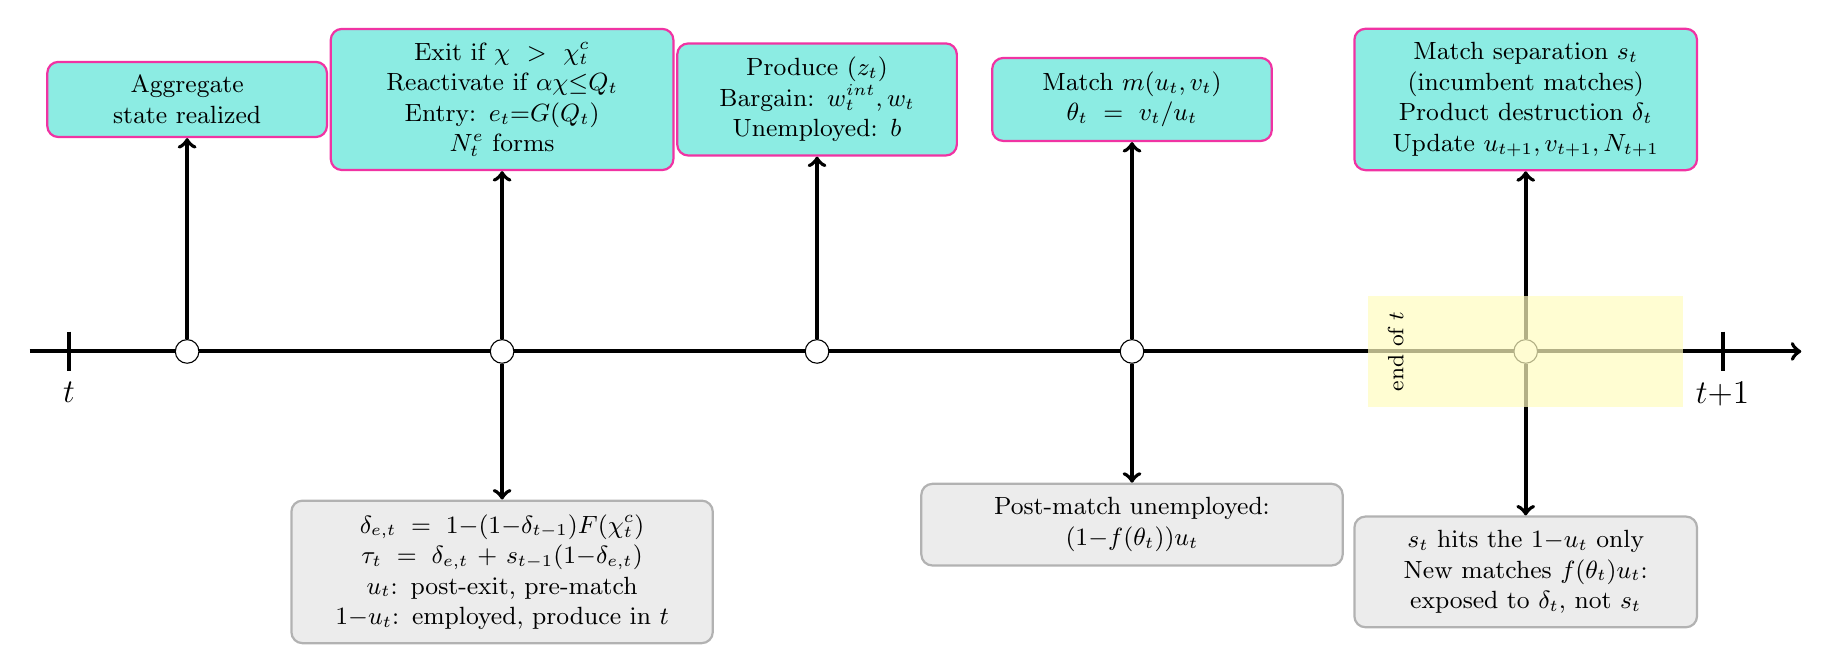
\begin{tikzpicture}[
				box/.style={draw=magenta!80, fill=turquoise!60, thick, rounded corners,
					align=center, font=\small, inner sep=5pt, text width=3.2cm},
				ebox/.style={draw=magenta!80, fill=turquoise!60, thick, rounded corners,
					align=center, font=\small, inner sep=5pt, text width=4.0cm},
				gbox/.style={draw=gray!60, fill=gray!15, thick, rounded corners,
					align=center, font=\small, inner sep=5pt, text width=5cm},
				dot/.style={circle, draw=black, fill=white, inner sep=0pt, minimum size=3mm},
				lw/.style={line width=0.5mm}]
				
				%% ── timeline ──
				\draw[lw,->] (-0.5,0) -- (22,0);
				\draw[lw] (0, 0.25) -- (0,-0.25) node[below]{\large$t$};
				\draw[lw] (21,0.25) -- (21,-0.25) node[below]{\large$t{+}1$};
				
				%% ── dots ──
				\node[dot] (d1) at (1.5,0) {};
				\node[dot] (d2) at (5.5,0) {};
				\node[dot] (d3) at (9.5,0) {};
				\node[dot] (d4) at (13.5,0) {};
				\node[dot] (d5) at (18.5,0) {};
				
				%% ── ABOVE: actions (alternating heights to avoid crowding) ──
				\node[box] (B1) at (1.5, 3.2)
				{Aggregate state realized};
				
				\node[ebox] (B2) at (5.5, 3.2)
				{Exit if $\chi>\chi_t^c$\\Reactivate if $\alpha\chi{\leq}Q_t$\\
					Entry: $e_t{=}G(Q_t)$\\$N_t^e$ forms};
				
				\node[box] (B3) at (9.5, 3.2)
				{Produce ($z_t$)\\Bargain: $w_t^{int},w_t$\\Unemployed: $b$};
				
				\node[box] (B4) at (13.5, 3.2)
				{Match $m(u_t,v_t)$\\$\theta_t=v_t/u_t$};
				
				\node[ebox] (B5) at (18.5, 3.2)
				{Match separation $s_t$\\(incumbent matches)\\
					Product destruction $\delta_t$\\
					Update $u_{t+1},v_{t+1},N_{t+1}$};
				
				%% ── BELOW: key implied stocks ──
				\node[gbox] (C1) at (5.5, -2.8)
				{$\delta_{e,t}=1{-}(1{-}\delta_{t-1})F(\chi_t^c)$\\
					$\tau_t=\delta_{e,t}+s_{t-1}(1{-}\delta_{e,t})$\\
					$u_t$: post-exit, pre-match\\
					$1{-}u_t$: employed, produce in $t$};

				\node[gbox] (C2) at (13.5, -2.2)
				{Post-match unemployed:\\$(1{-}f(\theta_t))u_t$};

				\node[gbox, text width=4.0cm] (C3) at (18.5, -2.8)
				{$s_t$ hits the $1{-}u_t$ only\\
					New matches $f(\theta_t)u_t$:\\
					exposed to $\delta_t$, not $s_t$};
				
				%% ── connectors ──
				\foreach \d/\B in {d1/B1, d2/B2, d3/B3, d4/B4, d5/B5}
				\draw[lw,->] (\d) -- (\B);
				
				\draw[lw,->] (d2) -- (C1);
				\draw[lw,->] (d4) -- (C2);
				\draw[lw,->] (d5) -- (C3);
				
				%% ── end-of-period shaded band ──
				\fill[yellow!25, opacity=0.7] (16.5,-0.7) rectangle (20.5,0.7);
				\node[font=\footnotesize, rotate=90] at (16.85,0) {end of $t$};
				
		\end{tikzpicture}}
		\caption{Timing. Turquoise: agent decisions. Grey: implied states. 
			Yellow band: shocks realizing end of $t$, governing $t{+}1$.
			Match separation applies only to matches in place at the
			start of $t$; matches formed in $t$ first face it at the end
			of $t{+}1$.}
		\label{fig:Timing}
	\end{figure}
	
	%%%%%%%%%%%%%%%%%%%%%%%%%%%%%%%%%%%%%%%%%%
	\section{Equilibrium}\label{sec:equilibrium}
	%%%%%%%%%%%%%%%%%%%%%%%%%%%%%%%%%%%%%%%%%%
	
	This section derives equilibrium and then shows that it comprises three blocks: a 
	business formation block governing the evolution of product lines 
	and firm values, a labor market block governing vacancy creation, 
	matching, and wage determination, and stochastic processes for 
	the three structural shocks. Table~\ref{tab:ingredients_comparison} 
	positions the paper relative to the closest antecedents across these dimensions. Section~\ref{sec:mechanism} derives 
	formally the asymmetric transmission of $\delta$ and $s$ shocks 
	that motivates the paper's empirical strategy.
	
	
	
	\subsection{Household problem}
	
	Let $\nu_t$ denote the ex-dividend equity price of the aggregate 
	firm portfolio and $\nu_t^f$ the post-dividend value of an 
	individual firm, following \citet{bilbiie_2012}. Given 
	risk-aversion parameter $\sigma$ and discount factor $\beta$, 
	the household chooses consumption $c_t$ and equity shares $a_t$ 
	to maximize expected discounted utility:
	\begin{align}
		\max_{c_t,\,a_t}\sum_{t=0}^{\infty}
		\mathbb{E}_0\,\beta^t c_t^{1-\sigma}/(1-\sigma)
	\end{align}
	subject to
	\begin{align}\label{eq:bc_HH}
		c_t + \nu_t a_{t+1} = w_t(1-u_t) + b u_t 
		+ (\nu_t+d_t)a_t + D_t^{int} - T_t
	\end{align}
	where $b$ is the value of unemployment, $d_t$ is the per-share 
	dividend, $D_t^{int}$ are intermediary dividends, and $T_t$ are 
	lump-sum taxes financing unemployment benefits. Since households 
	have unit mass, $c_t = C_t$ in equilibrium. The first-order 
	condition for equity shares yields the standard asset-pricing 
	equation:
	\begin{align}\label{eq:euler_shares}
		\lambda_t \nu_t = \beta\,\mathbb{E}_t\lambda_{t+1}
		[\nu_{t+1}+d_{t+1}]
	\end{align}
	where $\lambda_t = c_t^{-\sigma}$ is the marginal utility of 
	consumption and $m_{t+1}\equiv\beta(\lambda_{t+1}/\lambda_t)$ 
	is the stochastic discount factor. To express~\eqref{eq:euler_shares} 
	at the firm level, use the mappings $\nu_t=\nu_t^f(N_t+N_t^e)$ 
	and $\nu_t+d_t=(\nu_t^f+d_t^f)N_t$, together with the firm law 
	of motion~\eqref{eq:firm_law_motion}. This yields the firm-level 
	Euler equation, familiar from BGM and extended here to 
	incorporate endogenous exit:
	\begin{align}\label{eq:euler_firm}
		\nu_t^f = \mathbb{E}_t m_{t+1}(1-\delta_t)F(\chi_{t+1}^c)
		(\nu_{t+1}^f+d_{t+1}^f)
	\end{align}
	Equation~\eqref{eq:euler_firm} equates the current firm value to 
	the expected discounted sum of next-period firm value and 
	dividends, adjusted for the stochastic discount factor 
	$m_{t+1}$ and the survival probability $(1-\delta_t)F(\chi_{t+1}^c)$, 
	which combines the probability of surviving exogenous destruction 
	$(1-\delta_t)$ and the probability of drawing a continuation 
	cost below the equilibrium cutoff $\chi_{t+1}^c$, with probability $F(\chi_{t+1}^c)$.
	
	\subsection{Recruiters}
	\label{sec:recruiters}
	
	There is a fixed unit measure of recruiters who can create 
	vacancies subject to a sunk cost $x$ drawn from cdf $G(\cdot)$. 
	Additionally, if a vacancy is filled the recruiter pays a fixed 
	real cost $\kappa$ before bargaining with the newly matched 
	worker.\footnote{\citet{pissarides_2009} first suggested this 
		matching cost to make vacancy posting more responsive; 
		\citet{christiano_2016} estimate it accounts for the dominant 
		share of recruiting costs.} After matching, the recruiter rents 
	labor to an incumbent retailer with product line $j$. We 
	introduce recruiters as a separate agent type to avoid the 
	complications of Stole-Zwiebel intra-firm bargaining that arise 
	when workers negotiate directly with retailers facing a downward-
	sloping demand curve: with a separate recruiter, the bilateral 
	bargaining problem reduces to the standard DMP surplus-splitting 
	equation regardless of the retail market structure.\footnote{Under 
		Stole-Zwiebel bargaining, retailers would strategically over-hire 
		to improve their bargaining position, generating a fixed-point 
		problem in employment that significantly complicates aggregation. 
		The recruiter segmentation is isomorphic to the retailer--
		wholesaler structure of \citet{christiano_2016}, with recruiters 
		replacing intermediate goods.} Let $Q_t^j$ and $J_t^j$ denote 
	the values of an unfilled and filled vacancy associated with 
	product line $j$.
	
	The value of an unfilled vacancy for product line $j$ satisfies
	\begin{align}\label{eq:value_recruiter_unmatched}
		Q_{t}^j &= \mathbb{E}_t m_{t+1}(1-\delta_t)F(\chi_{t+1}^c)
		\bigl[(1-q(\theta_t))Q_{t+1}^j
		+q(\theta_{t})J_{t+1}^j\bigr]-q(\theta_t)\kappa \notag \\
		&= \mathbb{E}_t m_{t+1}(1-\delta_t)F(\chi_{t+1}^c)
		\bigl[Q_{t+1}^j+q(\theta_t)
		(J_{t+1}^j-Q_{t+1}^j)\bigr]-q(\theta_t)\kappa
	\end{align}
	An unmatched recruiter survives to next period only if the 
	product line survives both exogenous destruction and the 
	continuation-cost draw, with probability $(1-\delta_t)F(\chi_{t+1}^c)$. 
	In the next period, the vacancy fills with probability 
	$q(\theta_t)$, generating value $J_{t+1}^j$, or remains unfilled 
	with probability $1-q(\theta_t)$. The matching cost $\kappa$ 
	is paid upon filling. The recruiter chooses the best product 
	line: $Q_t\equiv\max_j Q_t^j$. In equilibrium, competition 
	equalizes values across active product lines: $Q_t^j=Q_t$ for 
	all $j$ with $v_t^j>0$.
	
	Define the flow value of a vacancy as the net benefit of 
	holding a vacancy this period relative to next:
	\begin{align}\label{eq:K}
		K_t \equiv Q_t - 
		\mathbb{E}_t m_{t+1}(1-\delta_t)F(\chi_{t+1}^c)Q_{t+1}
	\end{align}
	Inserting \eqref{eq:K} into \eqref{eq:value_recruiter_unmatched} and rearranging places the 
	average hiring cost on the left-hand side:
	\begin{align}\label{eq:average_hiring_cost}
		\kappa+\frac{K_t}{q(\theta_t)} = 
		\mathbb{E}_t m_{t+1}(1-\delta_t)F(\chi_{t+1}^c)
		(J_{t+1}^j-Q_{t+1})
	\end{align}
	
	A recruiter opens a vacancy whenever $x\leq Q_t$, so total 
	newly opened vacancies are $e_t=G(Q_t)$. Following CK, we 
	adopt a power law distribution:
	\begin{align}
		G(x)=\left(\frac{x}{x_m}\right)^{\xi}, 
		\quad x\in[0,\,x_m]
	\end{align}
	with density $g(x)=\xi x^{\xi-1}/x_m^{\xi}$.\footnote{If 
		$\xi>1$ the density is rising (relatively more high-cost 
		recruiters); if $\xi<1$ it is falling; if $\xi=1$ costs are 
		uniform on $[0,x_m]$.} Provided $Q<x_m$, inverting $e=G(Q)$ 
	gives
	\begin{align}\label{eq:Q}
		Q_t = e_t^{1/\xi}\,x_m
	\end{align}
	so the elasticity of the vacancy value with respect to entry 
	is $1/\xi$. The limit $\xi\to\infty$ is infinitely elastic vacancy creation, or vacancy
	free entry. It does not nest the DMP model with a flow vacancy cost, because the cost of a
	vacancy here is durable. Remark~\ref{rem:dmp} gives the exact relationship.
	
	By symmetry of the retail problem (established in 
	Section~\ref{sec:retailers}), recruiter compensation 
	$w_t^{int,j}$ and the value of a filled vacancy $J_t^j$ are 
	identical across active product lines; we henceforth drop the 
	superscript $j$. Recruiters supply labor in a competitive 
	market, taking $w_t^{int}$ as given. The value of a matched 
	recruiter is\footnote{The asset-pricing equations 
		\eqref{eq:value_recruiter_unmatched} and 
		\eqref{eq:value_recruiter_matched} can equivalently be obtained 
		by having the household purchase shares of recruiter firms 
		directly; the stochastic discount factor ensures equivalence. 
		Writing it via the household problem makes the derivation more 
		compact and facilitates comparison to BGM and 
		\citet{mortensen_1994}.}
	\begin{align}\label{eq:value_recruiter_matched}
		J_{t} = w_t^{int}-w_t + \mathbb{E}_{t}m_{t+1}
		(1-\delta_t)F(\chi_{t+1}^c)
		\bigl(s_t\, Q_{t+1}^{rep}+(1-s_t)J_{t+1}\bigr)
	\end{align}
	The recruiter receives $w_t^{int}$ from the retailer and 
	pays the worker $w_t$. Conditional on product-line survival, 
	the match continues with probability $1-s_t$. Otherwise the worker separates and the recruiter may reactivate the vacancy at cost $\alpha\chi$, with $\chi\sim F$ drawn from the same distribution as the continuation cost, scaled by $\alpha$. Reactivation is optimal when the recovered vacancy covers the cost, $Q_{t+1}\geq\alpha\chi$, which occurs with probability $\Lambda_{r,t+1}$, where the reactivation rate is
	\begin{align}\label{eq:Lambda_r}
		\Lambda_{r,t}\equiv F\!\left(\frac{Q_t}{\alpha}\right)
		=\min\left\{1-p_0+p_0\left(\frac{Q_t}{\alpha\chi_m}\right)^{\psi},\,1\right\}
	\end{align}
	using the form of $F$ in~\eqref{eq:F_chi}. $\Lambda_{r,t}\in[1-p_0,1]$, and every vacated position is reactivated once $Q_t\geq\alpha\chi_m$. The reactivation rate rises with $Q_t$ and so shares its cyclical behavior. The expected value of a separated position is therefore the reactivation option value
	\begin{align}\label{eq:Qrep}
		Q_t^{rep}\equiv\mathbb{E}\bigl[\max\{Q_t-\alpha\chi,\,0\}\bigr]
		= Q_t\Lambda_{r,t}-\alpha\int_{0}^{Q_t/\alpha}\chi\,dF(\chi),
	\end{align}
	the mass of reactivated vacancies valued at $Q_t$ net of the reactivation costs paid. Costless full reposting ($Q_t^{rep}=Q_t$) is nested as $\alpha\to0$.
	
	\paragraph{Job creation condition}
	Subtracting~\eqref{eq:value_recruiter_unmatched}
	from~\eqref{eq:value_recruiter_matched} and using the definition 
	of $K_t$ yields recruiter surplus:
	\begin{align}\label{eq:value_recruiter_surplus}
		J_t - Q_t &= w_t^{int}-w_t - K_t
		+ (1-s_t)\left(\kappa+\frac{K_t}{q(\theta_t)}\right)-s_t\mathcal{R}_t
	\end{align}
	where
	\begin{align}\label{eq:repost_shortfall}
		\mathcal{R}_t\equiv\mathbb{E}_tm_{t+1}(1-\delta_t)F(\chi_{t+1}^c)\left(Q_{t+1}-Q_{t+1}^{rep}\right)
	\end{align}
	is the expected discounted reposting shortfall: the value a separated position loses
	relative to costless reposting, through the positions that are retired and the
	reactivation costs paid on those that are not. It vanishes as
	$\alpha\to0$. Imposing symmetry
	in~\eqref{eq:average_hiring_cost} gives the job creation
	condition:
\begin{align}\label{eq:jcc}
	\kappa+\frac{K_t}{q(\theta_t)} = 
	\mathbb{E}_t m_{t+1}(1-\delta_t)F(\chi_{t+1}^c)
	\left(J_{t+1}-Q_{t+1}\right)
\end{align}
	The left-hand side is the average hiring cost: the fixed 
	matching cost $\kappa$ plus the flow cost $K_t/q(\theta_t)$, 
	equal to the opportunity cost of holding the vacancy this 
	period multiplied by its expected duration $1/q(\theta_t)$. 
	The right-hand side is the expected surplus of a match that
	begins producing next period, discounted by the stochastic
	discount factor and the product-line survival probability.
	By~\eqref{eq:value_recruiter_surplus}, that surplus is the
	recruiter's net revenue less the flow value of the vacancy,
	plus the hiring cost saved if the match survives separation,
	less the reposting shortfall if it does not.
	
	\subsection{Wage determination}
	
	Nash bargaining between the recruiter and worker yields
	\begin{align}\label{eq:wage_eq}
		w_t = \phi\left(w_t^{int} - K_t 
		+ f(\theta_t)\left(\kappa
		+\frac{K_t}{q(\theta_t)}\right)-s_t\mathcal{R}_t\right)
		+(1-\phi)b
	\end{align}
	where $\phi$ is the worker's bargaining power.\footnote{The 
		wage equation \eqref{eq:wage_eq} has the same general form as 
		\citet{shao_2013}, their equations 21 and 22. Their setting 
		includes capital affecting $w_t^{int}$ and writes the wage 
		using the vacancy value $Q_t$ rather than the flow value 
		$K_t$.} Recruiter compensation $w_t^{int}=\rho(N_t)z_t/
	\mu(N_t)$ — derived in Section~\ref{sec:retailers} — enters 
	negatively through the markup. The flow entry cost $K_t$ has 
	opposing effects: it reduces the match surplus (dampening 
	wages by $\phi K_t$) but improves the worker's threat point, 
	raising the tightness slope of the wage curve by $\phi\theta 
	K_t$; the second effect dominates when $\theta>1$. The fixed 
	cost $\kappa$ raises wages by $\phi f(\theta_t)\kappa$ because 
	a failed negotiation forces the firm to pay $\kappa$ again 
	upon next filling the vacancy. The reposting shortfall lowers
	the wage by $\phi s_t\mathcal{R}_t$: the expected loss of position value on separation works
	as an extra flow cost of holding a filled position, alongside $K_t$, and the worker bears
	share $\phi$ of it. The household's
	surplus carries no such term, because a separated worker
	becomes unemployed whether or not the position is reactivated
	(\ref{app:wage}). Setting $w_t^{int}=z_t$,
	$\kappa=0$, and $\alpha\to0$ recovers the CK wage equation.

	Substituting~\eqref{eq:wage_eq}
	into~\eqref{eq:value_recruiter_surplus} to eliminate $w_t$
	yields the wage-substituted surplus:
	\begin{align}\label{eq:surplus_wage}
		J_t-Q_t &= (1-\phi)\left(w_t^{int}-K_t-b\right)
		-\phi\theta_t\left(K_t+q(\theta_t)\kappa\right) \notag \\
		&\quad +(1-s_t)\left(\kappa+\frac{K_t}{q(\theta_t)}\right)
		-(1-\phi)s_t\mathcal{R}_t
	\end{align}
	The recruiter bears share $1-\phi$ of the reposting shortfall;
	the worker bears the rest through the wage.

	\subsection{Retailers}\label{sec:retailers}
	
	A retailer selling variety $j$ rents labor from recruiters at 
	wage $w_t^{int,j}$. At the beginning of each period, before 
	production, the firm draws a continuation cost $\chi\sim F$ from
	\eqref{eq:F_chi}. A firm with draw $\chi>\chi_t^c$ exits; one with $\chi\leq\chi_t^c$ 
	pays the cost and continues. Define the survival probability:
	\begin{align}\label{eq:Lambda}
		\Lambda_t \equiv F(\chi_t^c) = (1-p_0) 
		+ p_0\left(\frac{\chi_t^c}{\chi_m}\right)^\psi
	\end{align}
	so that the endogenous exit rate is $1-\Lambda_t = 
	p_0\left(1-(\chi_t^c/\chi_m)^\psi\right)$, consistent with the 
	total exit rate $\delta_{e,t}=1-(1-\delta_{t-1})\Lambda_t$ from 
	Section~\ref{sec:environment}. The elasticity of the endogenous 
	exit rate with respect to the cutoff is 
	$\psi p_0(\chi_t^c/\chi_m)^\psi/(1-\Lambda_t)$, which increases 
	in $\psi$ and falls as the mass point $1-p_0$ rises.
	
	The value of a firm after its cost realization is:
	\begin{align}\label{eq:firm_bellman}
		\nu_t^f(\chi) = \max\left\{0,\; 
		\max_{y_t}\left[\rho^d(y_t)y_t - 
		w_t^{int}\frac{y_t}{z_t}\right]
		-\chi + (1-\delta_t)\mathbb{E}_t m_{t+1}\Lambda_{t+1}
		\,\nu_{t+1}^{ef}\right\}
	\end{align}
	where $\nu_t^{ef}\equiv(1/\Lambda_t)\int_0^{\chi_t^c}
	\nu_t^f(\tilde{\chi})\,dF(\tilde{\chi})$ is the expected 
	firm value conditional on survival, and $\rho^d(y_t)$ is the 
	inverse demand curve from~\eqref{eq:demand}, equal in symmetric 
	equilibrium to $\rho(N_t)$. The profit maximization problem 
	is static: letting $MR\equiv\rho'(y)y+\rho(y)$ denote marginal 
	revenue, the first-order condition is
	\begin{align}\label{eq:retailer_optimality}
		MR_t\cdot z_t = w_t^{int,j}
	\end{align}
	The left-hand side is the marginal revenue product; the 
	right-hand side is recruiter compensation, which exceeds the 
	worker's wage due to matching frictions. Equivalently, 
	$MR_t = MC_t = w_t^{int}/z_t$. The standard markup condition 
	$\rho(N_t) = \mu(N_t)MC_t$ gives recruiter compensation:
	\begin{align}\label{eq:recruiter_compensation}
		w_t^{int} = \frac{\rho(N_t)}{\mu(N_t)}z_t
	\end{align}
	Recruiter compensation is increasing in the relative price 
	$\rho(N_t)$ and technology $z_t$ and decreasing in the markup 
	$\mu(N_t)$. Since $\mu'(N_t)\leq 0$, $w_t^{int}$ is 
	increasing in $N_t$ overall.\footnote{Following BGM, marginal 
		cost is $w_t^{int}/z_t$. Under DS-CES, $\mu=\varepsilon/
		(\varepsilon-1)$ is constant, recovering the standard formula.} 
	Retail profits gross of the continuation cost are a share 
	$(\mu(N_t)-1)/\mu(N_t)$ of sales:
	\begin{align}\label{eq:retail_profits}
		R_t^f = \frac{\mu(N_t)-1}{\mu(N_t)}\rho(N_t)y_t
	\end{align}
	
	\subsection{Firm entry and exit}\label{sec:entry_exit}
	
	By definition $\nu_t^f(\chi_t^c)=0$. Evaluating 
	the firm Bellman~\eqref{eq:firm_bellman} at 
	$\chi=\chi_t^c$ yields the cutoff condition:
	\begin{align}\label{eq:cutoff}
		\chi_t^c = R_t^f + \nu_t^f
	\end{align}
	where $\nu_t^f\equiv\nu_t^{ef}\cdot\Lambda_t$ is the 
	unconditional expected firm value. From the Bellman, 
	the firm value conditional on the cost realization is 
	$\nu_t^f(\chi)=\chi_t^c-\chi$ for all $\chi\leq\chi_t^c$, 
	so that $\nu_t^{ef}=\chi_t^c - E(\chi\,|\,\chi\leq\chi_t^c)$. 
	For the power law component, the conditional mean of a 
	positive draw satisfies $E(\chi\,|\,0<\chi\leq\chi_t^c)
	=\psi_c\chi_t^c$ where $\psi_c\equiv\psi/(\psi+1)$, 
	and positive draws are a share $p_0(\chi_t^c/\chi_m)^\psi/\Lambda_t$ of the draws below
	the cutoff, so the overall conditional mean (including the mass point at zero) is
	$E(\chi\,|\,\chi\leq\chi_t^c)=p_0\psi_c\chi_t^c(\chi_t^c/\chi_m)^\psi/\Lambda_t$.
	Hence:
	\begin{align}\label{eq:firm_value_char}
		\nu_t^f = (1-\delta_t)\mathbb{E}_t m_{t+1}
		\Lambda_{t+1}\,\nu_{t+1}^{ef}
	\end{align}
	
	New firms are created using technology $N_t^e=z_t l_t^e/f_e$, 
	where $l_t^e$ is labor hired from recruiters at wage 
	$w_t^{int}$ and $f_e$ is the sunk entry cost in labor units, 
	equivalent to $w_t^{int}f_e/z_t=\rho(N_t)f_e/\mu(N_t)$ 
	units of the consumption basket. Firms enter until the 
	post-dividend firm value equals the sunk entry cost:
	\begin{align}\label{eq:free_entry}
		\nu_t^f = \frac{\rho(N_t)f_e}{\mu(N_t)}
	\end{align}
	Combining the free entry condition~\eqref{eq:free_entry} 
	with the cutoff condition~\eqref{eq:cutoff} yields:
	\begin{align}\label{eq:cutoff_free_entry}
		\chi_t^c = R_t^f + \frac{\rho(N_t)f_e}{\mu(N_t)}
	\end{align}
	The cutoff rises with current profitability $R_t^f$ and 
	the value of a new product line $\rho(N_t)f_e/\mu(N_t)$: 
	when conditions improve, marginal firms that would 
	otherwise exit find it worthwhile to continue.
	\subsection{Aggregation}\label{sec:aggregation}
	
	Labor market clearing implies $L_t = 1-u_t$. Define 
	gross consumption output $Y_t^c \equiv \rho(N_t)N_t y_t$ 
	and retail employment $L_t^c \equiv N_t l_t^c$. Aggregate 
	continuation costs paid by surviving firms are
	\begin{align}\label{eq:agg_fixed_costs}
		X_t^c \equiv (1-\delta_{t-1})(N_{t-1}+N_{t-1}^e)\int_0^{\chi_t^c}\chi\,dF(\chi)
		= N_t\,E(\chi\,|\,\chi\leq\chi_t^c)
		= N_t\,\psi_c\,\chi_t^c\,\frac{p_0}{\Lambda_t}
		\left(\frac{\chi_t^c}{\chi_m}\right)^{\psi}
	\end{align}
	where $\psi_c\equiv\psi/(\psi+1)$. Every line that survives exogenous destruction draws a
	cost, and those drawing $\chi>\chi_t^c$ exit and pay nothing, so the pre-exit mass
	multiplies the partial expectation. Since $N_t=\Lambda_t(1-\delta_{t-1})(N_{t-1}+N_{t-1}^e)$,
	this is the surviving mass times the conditional mean. The factor
	$p_0(\chi_t^c/\chi_m)^\psi/\Lambda_t$ is the share of survivors that drew a positive cost.
	
	Aggregate reactivation costs are paid by surviving firms that resume a position vacated at the end of $t-1$:
	\begin{align}\label{eq:agg_repost_costs}
		X_t^r \equiv (1-\delta_{e,t})\,s_{t-1}(1-u_{t-1})
		\int_0^{Q_t/\alpha}\alpha\chi\,dF(\chi)
	\end{align}
	Only the power-law part of $F$ contributes, since the atom at zero carries no cost, so the
	per-position integral is
	$\int_0^{Q_t/\alpha}\alpha\chi\,dF(\chi)=\psi_cQ_t\,p_0\bigl(Q_t/(\alpha\chi_m)\bigr)^{\psi}
	=\psi_cQ_t(\Lambda_{r,t}-1+p_0)$, using the interior branch of~\eqref{eq:Lambda_r}. The
	cost scale $\alpha$ survives only through $\Lambda_{r,t}$. The count in
	\eqref{eq:agg_repost_costs} omits $\Lambda_{r,t}$ because the integral is a partial
	expectation, which already embeds the reactivation probability. As $\Lambda_{r,t}\to1-p_0$,
	only the zero-cost atom reactivates and $X_t^r\to0$.

	Aggregate retail profits 
	gross of continuation costs are $\Pi_t^f = Y_t^c/
	\varepsilon(N_t) - X_t^c$, and recruiter profits, net of the
	vacancy creation and matching costs $X_t$ and the reactivation
	costs $X_t^r$ that recruiters pay, are
	$\Pi_t^{int} = (w_t^{int}-w_t)L_t-X_t-X_t^r$. The average per-firm
	dividend is $d_t^f = \Pi_t^f/N_t$.
	
	Total vacancy creation costs are the sum of sunk posting 
	costs and fixed matching costs:
	\begin{align}\label{eq:X_total}
		X_t = X_v + X_f 
		= e_t\frac{\xi}{\xi+1}Q_t + \kappa q(\theta_t)v_t
	\end{align}
	where $X_v = x_m^{-\xi}\frac{\xi}{\xi+1}Q_t^{\xi+1}$ 
	follows from integrating $xg(x)$ over $[0,Q_t]$. Given 
	$e_t$ and $Q_t$, the parameter $x_m$ has no additional 
	effect on entry costs provided $Q_t < x_m$.
	
	Aggregating~\eqref{eq:bc_HH} with asset market clearing 
	$a_{t+1}=a_t$ and $T_t=bu_t$, and using 
	$Y_t^{Gross} = Y_t^c + \nu_t^f N_t^e$, real GDP net 
	of intermediate inputs is:
	\begin{align}\label{eq:gdp}
		Y_t \equiv Y_t^{Gross} - X_t - X_t^c -X_t^r
		= C_t + \nu_t^f N_t^e 
		= w_tL_t + \Pi_t^f + \Pi_t^{int}
	\end{align}
	GDP comprises consumption and investment in new product 
	lines. Moreover, decomposing output into income confirms the national 
	accounts identity.
	
	Using free entry~\eqref{eq:free_entry} and $d_t^f = 
	\Pi_t^f/N_t$, the firm-level Euler 
	equation~\eqref{eq:euler_firm} becomes the business 
	formation equation:
	\begin{align}\label{eq:euler_bf}
		f_e\rho(N_t) = (1-\delta_t)\mathbb{E}_t m_{t+1}
		\Lambda_{t+1}\frac{\mu(N_t)}{\mu(N_{t+1})}
		\left\{f_e\rho(N_{t+1}) + \frac{Y_{t+1}^c}{N_{t+1}}
		\left(\mu(N_{t+1})-1-\mu(N_{t+1})
		\frac{X_{t+1}^c}{Y_{t+1}^c}\right)\right\}
	\end{align}
	The left-hand side is the current cost of creating a 
	product line. The right-hand side is the expected 
	discounted return, adjusted for survival probability 
	$(1-\delta_t)\Lambda_{t+1}$ and the current-to-future 
	markup ratio $\mu(N_t)/\mu(N_{t+1})$. The term in 
	braces is the next-period firm value plus the private 
	marginal product of a new product line net of 
	continuation costs; the net markup $\mu(N_{t+1})-1$ 
	governs the return to entry.
	
	\subsection{Definition of equilibrium}\label{sec:def_eq}
	
	\begin{definition}\label{def:equilibrium}
		Given $\rho(N)$, $\mu(N)$, $F$, initial exogenous
		states $\{z_0,\delta_{-1},s_{-1}\}$, and initial endogenous
		states $\{v_{-1},u_{-1},B_{-1}\}$, where
		$B_{-1}\equiv N_{-1}+N^e_{-1}$ is the stock of product lines
		entering period~0 before exit, an equilibrium is
		a sequence $\{N_t, C_t, \chi_t^c, Y_t^c, \theta_t,
		K_t, Q_t, e_t, v_t, u_t\}_{t=0}^\infty$ satisfying the
		business formation block:
		\begin{align}
			\label{eq:N_lom_eq}
			N_t &= (1-\delta_{t-1})\Lambda_t
			\left(N_{t-1} + \frac{z_{t-1}(1-u_{t-1})}{f_e}
			- \frac{Y_{t-1}^c}{f_e\rho(N_{t-1})}\right) \\
			\label{eq:N_euler_eq}
			f_e\rho(N_t) &= (1-\delta_t)\mathbb{E}_t 
			m_{t+1}\Lambda_{t+1}
			\frac{\mu(N_t)}{\mu(N_{t+1})}
			\left\{f_e\rho(N_{t+1}) + \frac{Y_{t+1}^c}{N_{t+1}}
			\left(\mu(N_{t+1})-1-\mu(N_{t+1})
			\frac{X_{t+1}^c}{Y_{t+1}^c}\right)\right\} \\
			\label{eq:rc}
			Y_t^c &= C_t + X_t + X_t^c+X_t^r \\
			\label{eq:cutoff_eq}
			\chi_t^c &= \frac{Y_t^c(\mu(N_t)-1)}{\mu(N_t)N_t} 
			+ \frac{f_e\rho(N_t)}{\mu(N_t)}
		\end{align}
		and the labor market block:
		\begin{align}
			\label{eq:jcc_eq}
			\kappa+\frac{K_t}{q(\theta_t)} &=
			\mathbb{E}_t m_{t+1}(1-\delta_t)\Lambda_{t+1}
			\Biggl[(1-\phi)\left(\frac{\rho(N_{t+1})z_{t+1}}
			{\mu(N_{t+1})}-K_{t+1}-b\right)
			-\phi\theta_{t+1}\left(K_{t+1}+q(\theta_{t+1})\kappa\right)
			\notag \\
			&\qquad +(1-s_{t+1})\left(\kappa
			+\frac{K_{t+1}}{q(\theta_{t+1})}\right)
			-(1-\phi)s_{t+1}\mathcal{R}_{t+1}\Biggr] \\
			\label{eq:Kdef}
			K_t &= Q_t - (1-\delta_t)\mathbb{E}_t 
			m_{t+1}\Lambda_{t+1}Q_{t+1} \\
			\label{eq:entry_eq}
			e_t &= \left(\frac{Q_t}{x_m}\right)^\xi \\
			\label{eq:theta_eq}
			\theta_t &= \frac{v_t}{u_t}
		\end{align}
		together with laws of motion
		\eqref{eq:u_lom}--\eqref{eq:v_lom}, auxiliary
		definitions $\delta_{e,t}$ \eqref{eq:delta_e_lom},
		$\tau_t$ \eqref{eq:tau_lom}, $\Lambda_t$
		\eqref{eq:Lambda}, $\Lambda_{r,t}$ \eqref{eq:Lambda_r},
		matching rates $f(\theta_t)=A\theta_t^{1-\eta_L}$ and
		$q(\theta_t)=A\theta_t^{-\eta_L}$,
		$Q_t^{rep}$ \eqref{eq:Qrep},
		$\mathcal{R}_t$ \eqref{eq:repost_shortfall},
		$X_t$ \eqref{eq:X_total}, $X_t^c$
		\eqref{eq:agg_fixed_costs}, $X_t^r$
		\eqref{eq:agg_repost_costs}, $m_t$
		\eqref{eq:euler_shares}, and
		stochastic processes \eqref{eq:ar1_z}--\eqref{eq:ar1_s}.
	\end{definition}
	
	The job creation condition substitutes the wage-substituted surplus~\eqref{eq:surplus_wage},
dated $t+1$, into~\eqref{eq:jcc}, so the matched value $J_t$ and the wage drop out.
Carrying the reposting shortfall $\mathcal{R}_t$ as a variable with its own one-period
equation~\eqref{eq:repost_shortfall} keeps the system first order, without a nested
expectation. The two blocks interact through $\rho(N_t)$ and $\mu(N_t)$ in the job creation
condition and through $\delta_t$ in the survival-adjusted discount factor
$(1-\delta_t)\Lambda_{t+1}$, which appears in both.

\subsection{Limiting cases}

Like \citet{coles_2018}, we study a destruction shock that removes jobs and vacancies together, and, like \citet{gabrovski_2025}, we consider separations that pertain to matches as well as business opportunities. However, those articles abstract from product variety and entry/exit decisions. This subsection connects the two settings. It
first states when the labor market block can be solved on its own. It then constructs the
benchmark economy against which the baseline is compared, and shows that this benchmark is
a limit of the baseline. That limit is where the analytical results of
Section~\ref{sec:mechanism} are proved. It closes by relating the business formation block
to \citet{bilbiie_2012}. Proofs are in \ref{app:limiting_cases}.

\begin{proposition}[Independence of labor market block]
	\label{prop:independence}
	Consider general CES preferences with elasticity of
	substitution $\varepsilon$. The labor market
	block $\{u_{t+1}, v_t, e_t, Q_t, K_t, J_t, w_t\}_{t=0}^{\infty}$
	can be solved independently of the business formation
	block for all values of the remaining parameters if and only if $\sigma=0$, $\zeta=0$,
	and $p_0=0$.
\end{proposition}

When $\sigma=0$, risk neutrality fixes $m_{t+1}=\beta$, 
eliminating the consumption dependence of the stochastic 
discount factor. When $\zeta=0$, the taste for variety 
vanishes and $\rho(N_t)=1$, removing $N_t$ from recruiter 
compensation $w_t^{int}=\rho(N_t)z_t/\mu(N_t)$ and from 
the job creation condition while leaving $\mu$ and hence 
the business formation block otherwise intact. Setting
$p_0=0$ makes $F$ a point mass at zero. This removes both endogenous exit ($\Lambda_t=1$ and
$\delta_{e,t}=\delta_{t-1}$) and partial reposting ($\Lambda_{r,t}=1$, $Q_t^{rep}=Q_t$, and $X_t^r=0$). That is,
every vacated position is resumed at no cost and the
reposting margin disappears along with the exit margin.\footnote{Had
reactivation costs been drawn from a separate distribution,
a fourth condition would have been required to shut down both margins.} Under all three conditions, the labor market block 
closes on its own; the business formation block then 
determines $C_t$ and $N_t$ taking $u_t$ and $X_t$ as 
given from the labor market block.
\paragraph{Clone replacement}
The benchmark must keep the destruction flow, the channel that \citet{coles_2018} and
\citet{gabrovski_2025} study, while abstracting from the decisions to enter and to exit.
We operationalize this with \emph{clone replacement}. Product lines
are destroyed at the rate $\delta_t$, as in the baseline, and destruction still eliminates
every position attached to the line. Each destroyed line is immediately replaced by an
identical one, at no resource cost, so the mass of lines stays at $N_t=1$ at all dates. Two
things follow. There is no business formation margin, because entry is not a decision.
And there is no variety effect, because $N_t$ never moves and $\rho=\mu=1$. What survives
is the destruction channel itself. Since $\Lambda_t=1$ implies $\delta_{e,t}=\delta_{t-1}$,
$\delta_t$ is purely exogenous, and it still operates as a shock to jobs and vacancies.

Because replacement is costless, $\nu_t^fN_t^e$ drops out of the resource constraint. The
construction also sets $p_0=0$, so it removes the reactivation margin along with
endogenous exit.

\begin{proposition}[Clone-replacement equilibrium]
	\label{prop:ags}
	Under clone replacement with $N_t=1$ and $\mu=1$, 
	the business formation block drops out and equilibrium 
	labor market variables 
	$\{u_{t+1},v_t,e_t,Q_t,K_t\}_{t=0}^\infty$ satisfy:
	\begin{align}
		\label{eq:jcc_ags}
		\kappa+\frac{K_t}{q(\theta_t)} &= 
		\mathbb{E}_t m_{t+1}(1-\delta_t)
		\left((1-\phi)(z_{t+1}-K_{t+1}-b) \right.\notag\\
		&\quad\left. -\phi\theta_{t+1}
		(K_{t+1}+q(\theta_{t+1})\kappa)
		+(1-s_{t+1})\left(\kappa+
		\frac{K_{t+1}}{q(\theta_{t+1})}\right)\right)\\
		\label{eq:K_ags}
		K_t &= Q_t-(1-\delta_t)\mathbb{E}_t 
		m_{t+1}Q_{t+1}\\
		\label{eq:v_ags}
		v_t &= (1-\delta_{t-1})
		\left[(1-q(\theta_{t-1}))v_{t-1}
		+s_{t-1}(1-u_{t-1})\right]+e_t\\
		\label{eq:u_ags}
		u_t &= \left[1-(1-\delta_{t-1})f(\theta_{t-1})\right]u_{t-1}
		+\tau_t(1-u_{t-1})
	\end{align}
	together with $e_t=G(Q_t)$,
	$m_t=\beta(C_t/C_{t-1})^{-\sigma}$,
	\begin{equation}\label{eq:rc_limit}
		C_t = z_t(1-u_t)-X_t,
	\end{equation}
	and stochastic processes
	\eqref{eq:ar1_z}--\eqref{eq:ar1_s}, with
	$\delta_{e,t}=\delta_{t-1}$ since endogenous exit
	is absent by construction, and hence
	$\tau_t=\delta_{t-1}+s_{t-1}(1-\delta_{t-1})$.
\end{proposition}
We dub this the \emph{augmented Gabrovski-Silva} (AGS) model. Remark~\ref{rem:nesting}
makes the connection to the two papers precise.

\begin{remark}[Nested special cases of AGS]
	\label{rem:nesting}
	The AGS model nests two benchmark frameworks as
	limiting cases. Setting $\sigma=\kappa=0$ renders
	the AGS system isomorphic to \citet{gabrovski_2025},
	extended here with aggregate AR(1) shocks to
	$\delta_t$ and $s_t$.
	Additionally setting $s_t=0$ recovers
	\citet{coles_2018} exactly, with $w_t^{int}=z_t$. Both papers allow a flow cost of
	posting an unfilled vacancy and set it to zero in their quantitative work, as AGS does.
	Consumption is determined residually from
	$z_t(1-u_t)=C_t+e_t\frac{\xi}{\xi+1}Q_t$, which is \eqref{eq:X_total} with $\kappa=0$.
\end{remark}
\paragraph{AGS as a limit of the baseline}
Clone replacement is a heuristic. It supplies new product lines by fiat, so on its own it
does not say whether AGS is a special case of our economy or a different model. The
question matters because the results under vacancy free entry in Section~\ref{sec:mechanism} are proved
in AGS. The natural route is the limit in which variety stops mattering. Under DS-CES the
taste for variety vanishes as $\varepsilon\to\infty$, which delivers the condition
$\zeta=0$ of Proposition~\ref{prop:independence}. That single limit fails here, and the
reason is economic: business formation requires profits. Free entry equates the value of
a line to $\rho(N_t)f_e/\mu(N_t)$, and under DS-CES the markup that generates profit per
line is the taste for variety, $\mu-1=\zeta=1/(\varepsilon-1)$
(Section~\ref{sec:introduction}). With $f_e$ fixed, profits vanish as
$\varepsilon\to\infty$ while entry costs do not, so entry stops and $N\to0$. Gross output
$Y_t^c=\rho(N_t)N_ty_t$ then goes to zero with positive employment, and the limit is
degenerate.\footnote{Letting $\delta\to0$ as well would restore a positive mass of lines,
but it removes the destruction margin that the benchmark is meant to preserve.} Entry
costs must vanish with profits. Proposition~\ref{prop:double_limit} shows that scaling
$f_e=\bar{f}_e/\varepsilon$ as $\varepsilon\to\infty$ keeps the mass of lines finite and
positive while making business formation irrelevant for allocations.

\begin{proposition}[Double limit]
	\label{prop:double_limit}
	Consider DS-CES preferences. Set $p_0=0$, and let 
	$\varepsilon\to\infty$ jointly with $f_e=\bar{f}_e/
	\varepsilon$ for fixed $\bar{f}_e>0$. Then: \emph{(i)} the product-line mass has the unique
	steady-state value
	$\bar{N}=\bar{z}\bar{L}(1-\bar\delta)/[\bar{f}_e(r+\bar\delta)]>0$, and along any
	equilibrium path with entry interior ($N^e_t>0$) it is set period by period,
	\begin{equation}\label{eq:N_rule_limit}
		N_{t+1}=\frac{(1-\delta_t)\,\mathbb{E}_t[m_{t+1}z_{t+1}]\,(1-u_{t+1})}
		{\bar{f}_e\bigl[1-(1-\delta_t)\,\mathbb{E}_t m_{t+1}\bigr]};
	\end{equation}
	\emph{(ii)} firm
	value $\nu_t^f$, investment $\nu_t^f N_t^e$, and 
	labor devoted to entry $l_t^e$ all vanish at rate 
	$1/\varepsilon$; \emph{(iii)} recruiter compensation 
	$w_t^{int}\to z_t$; and \emph{(iv)} aggregate 
	allocations $\{\theta_t, u_t, v_t, C_t, Y_t^c\}$ 
	are independent of $\bar{f}_e$ and hence of $\bar{N}$, so the normalization
	$\bar{N}=1$, which corresponds to $\bar{f}_e=\bar{z}\bar{L}(1-\bar\delta)/(r+\bar\delta)$, is without loss of generality for
	aggregate allocations. In the limit, the business
	formation block is irrelevant to real allocations.
\end{proposition}

Every input to \eqref{eq:N_rule_limit} is a labor market object or a shock, so causation
runs one way: the labor market sets the mass of product lines, and the mass of product
lines feeds nothing back. Product variety still moves in the limit. A destruction shock
raises the user cost $r+\delta_t$ of a product line and lowers the target $N_{t+1}$. It
simply has no effect on allocations. This is the sense in which the clone-replacement
economy of Proposition~\ref{prop:ags}, which fixes $N_t=1$, implements the limit: it is the
limit for allocations, not for $N_t$.

The limit is stronger than the separability of Proposition~\ref{prop:independence}. The
labor market block does not merely close on its own: business formation leaves no trace
on allocations. Two consequences follow. First, the vacancy-free-entry results of
Section~\ref{sec:mechanism}, Lemma~\ref{lem:theta} and Proposition~\ref{prop:fe}, are
statements about the baseline economy in this limit, with $\sigma=\kappa=0$, not about a
different model. The proposition concerns the equilibrium conditions. It does not show
that impulse responses converge, so those results describe the limit economy, not the rate
at which the baseline approaches it. Second, the limit identifies what the comparison with
AGS measures. Away from it, entry costs do not vanish with profits, and business formation
works through the channels below.

The baseline differs from AGS in three respects, and only the first is a matter of
transmission channels. First, four objects move in the baseline labor market block
and are constant in AGS. Variety effects enter the job
creation condition through $\rho(N_t)/\mu(N_t)$. Profit
dilution enters the return to entry through $Y_t^c/N_t$ in
\eqref{eq:euler_bf}: a larger mass of lines lowers profit
per line, which regulates entry and feeds the survival
cutoff $\chi_t^c$ through current profitability $R_t^f$.
Endogenous exit operates through variation in that cutoff.
Partial reactivation operates through $\Lambda_{r,t}$, which
AGS loses because clone replacement sets $p_0=0$. Dilution
is distinct from the variety effect. It works through the
level of per-line profit rather than through the
welfare-based relative price, so it survives when $\rho$ is
held at unity. The four are developed formally in
Section~\ref{sec:mechanism} and evaluated quantitatively in
Section~\ref{sec:quantitative}.

Second, and more basic, AGS does not price replacement.
Clone replacement supplies a new line for every line
destroyed, at no resource cost, within the period, and in
every state of the world. The baseline makes each of these
an equilibrium outcome of \eqref{eq:euler_bf}. Entry absorbs
labor at rate $f_e$ and so enters the resource constraint
through $\nu_t^f N_t^e$ in \eqref{eq:gdp}, the mass of lines
is a slow-moving state, and the rate of replacement is an
equilibrium object rather than a constant. In the data replacement is slowest when
destruction is heaviest (Section~\ref{sec:introduction}). AGS holds the replacement
margin at its frictionless benchmark, so it cannot generate
the joint behavior of the two margins that motivates the
paper.

Third, AGS collapses measured and structural destruction.
Since $\Lambda_t=1$ implies $\delta_{e,t}=\delta_{t-1}$, the
realized destruction rate is the shock. In the baseline the
two differ by the endogenous exit margin, and it is the sum
that the establishment death rate of
Section~\ref{sec:empirical} measures.

A single comparison with AGS moves all of these at once. The quantitative work of
Section~\ref{sec:mechanism_irfs} therefore isolates the channels one at a time.

The business formation block, in turn, connects the model to \citet{bilbiie_2012}. The
baseline does not nest their model, since it has no intensive labor margin, but it nests a
restricted version. Define \emph{labor-restricted BGM} (LR-BGM) as the
\citet{bilbiie_2012} model with labor dropped from preferences: the household maximizes
$\sum_t \beta^t c_t^{1-\sigma}/(1-\sigma)$ subject to $c_t = w_t L_t + \pi_t - X_t$, where
$\{L_t\}$ and $\{X_t\}$ are exogenous sequences and $X_t$ is the vacancy-creation cost,
absorbed as an intermediate input.

\begin{remark}[Nesting LR-BGM]
	\label{rem:bgm_nest}
	Set $p_0=0$, so $X_t^c=0$, $\Lambda_t=1$, and
	$\delta_{e,t}=\delta_{t-1}$.  For any exogenous
	sequences $\{L_t\}$ and $\{X_t\}$, the business
	formation block of the baseline model---equations
	\eqref{eq:N_lom_eq}, \eqref{eq:N_euler_eq}, and
	\eqref{eq:gdp}---is isomorphic to LR-BGM evaluated
	at the same sequences.
\end{remark}

The isomorphism holds at the level of GDP \eqref{eq:gdp} rather than gross output
\eqref{eq:rc}. Vacancy costs $X_t$ are intermediate inputs in both models and cancel from
the resource constraint, leaving $Y_t = C_t + \nu_t^f N_t^e$ in each case. The only
departure from LR-BGM is that $L_t$ and $X_t$ are endogenous, determined by the labor
market block \eqref{eq:u_lom}--\eqref{eq:v_lom}. Restoring $p_0>0$ adds endogenous exit to
the LR-BGM core.

\begin{remark}[Dilution, variety, and the units of costs]\label{rem:dilution_variety}
	Under DS-CES, profit per line in goods, $(\mu-1)Y_t^c/(\mu N_t)$ with
	$Y_t^c=\rho(N_t)z_tL_t^c$, has elasticity $(2-\varepsilon)/(\varepsilon-1)$ in $N_t$. It
	combines a dilution effect of $-1$ and a variety effect of $1/(\varepsilon-1)$, which
	cancel at $\varepsilon=2$. Which effects matter depends on whether costs are paid in labor
	or goods, and on endogenous exit. Determinacy requires $\varepsilon$ above a threshold
	that exceeds 2 (\ref{app:determinacy}).
\end{remark}

\subsection{Shock transmission and the \texorpdfstring{$\delta$--$s$}{delta-s} asymmetry}\label{sec:mechanism}

The equilibrium laws of motion imply qualitatively distinct labor-market dynamics under
product destruction and under match separation. This section establishes the asymmetry
analytically, in three results, and then discusses partial reposting. The first gives necessary and sufficient conditions for the Beveridge curve to slope negatively in response to each shock in a special case of the AGS economy with
infinitely elastic vacancy creation. In this case, the labor market is block recursive and we can obtain analytic policy functions for the log linearized system. The second is an accounting result at horizon $h=1$ that holds for any entry
elasticity. The third extends the separation-shock result to endogenous exit. Negative
$u$--$v$ comovement can come from $\delta$ shocks, which destroy positions together with
matches, or from partial reposting, which turns part of each separation into position
destruction. The model contains both, and the quantitative analysis assesses their
relative contributions.

\paragraph{Infinitely elastic vacancy creation}
Consider the AGS economy of Proposition~\ref{prop:ags} with $\sigma=\kappa=0$, which by
Remark~\ref{rem:nesting} is \citet{gabrovski_2025} with aggregate shocks to $\delta_t$ and
$s_t$. Its labor market block closes on its own. Write $\delta_t=\bar\delta e^{\tilde\delta_t}$
and $s_t=\bar{s}e^{\tilde{s}_t}$, and consider one shock at a time, with persistence
$\rho_x\in[0,1)$ for $x\in\{\delta,s\}$.

\begin{assumption}[Infinitely elastic vacancy creation]\label{ass:vacancy_fe}
	\leavevmode
	\begin{enumerate}
		\item[(V1)] \emph{Vacancy free entry:} $\xi\to\infty$, so $Q_t=x_m$, and entry is
		interior, $e_t>0$.
		\item[(V2)] \emph{Separation margins:} $0<\bar\delta\leq\bar\tau$, with
		$\bar\delta<\bar\tau$ whenever the separation shock is considered.
		\item[(V3)] \emph{Unemployment persistence:} $(1-\bar\delta)\bar{f}+\bar\tau<1$.
	\end{enumerate}
\end{assumption}
\noindent Under (V2) both separation margins are present when $\bar\delta<\bar\tau$. The
destruction-shock results also hold at $\bar\delta=\bar\tau$, where there is no separation
margin. (V3) makes unemployment a persistent state, as shown below.

Vacancy free entry pins the price of a vacancy, not its flow value. By \eqref{eq:K_ags},
\begin{equation}\label{eq:K_user_cost}
	K_t=x_m\,\frac{r+\delta_t}{1+r},
\end{equation}
the user cost of an asset that destruction depreciates. In \citet{gabrovski_2025}
$\delta$ is constant, so vacancy free entry fixes $K$ as well. Here $K_t$ moves with the
exogenous $\delta_t$ and with nothing else, so the job creation condition
\eqref{eq:jcc_ags} contains only tightness and the shocks. This is what makes the
economy tractable: tightness can be solved without reference to unemployment or the
vacancy stock.

\begin{remark}[Relation to the DMP model]\label{rem:dmp}
Under Assumption~\ref{ass:vacancy_fe}, the labor market block is isomorphic to a DMP economy
with the same timing and separation margins in which every position, vacant or filled,
bears the flow user cost $K_t$ in \eqref{eq:K_user_cost}: posting a vacancy costs $K_t$ per
period, and output per match is $z_t-K_t$. With these substitutions the Nash wage
$\phi(z_t-K_t+\theta_tK_t)+(1-\phi)b$ and the job creation condition \eqref{eq:jcc_ags}
coincide with their DMP counterparts, the unemployment law of motion is the same, and
vacancies $v_t=\theta_tu_t$ jump with tightness because entry $e_t$ absorbs the
predetermined stock. The predetermined stock matters only if the entry constraint
$e_t\geq0$ binds.
\end{remark}

The isomorphism has two limits. First, under destruction shocks the DMP counterpart is
not the standard one. Its flow cost and net output move with $\delta_t$, and this
indexation is the user-cost channel behind the results below. With $\delta$ constant, $K$
is constant and the economy is DMP with a relabeled productivity, so technology and
separation shocks are transmitted as in DMP. Second, entry cannot be negative. A large
destruction shock lowers desired vacancies by more than destruction lowers the inherited
stock, entry stops, $Q_t$ falls below $x_m$, and the predetermined stock becomes a state.
This is the irreversibility of vacancy investment, which a flow-cost economy does not have.
The results below are local and assume interior entry.

\begin{lemma}[Tightness under vacancy free entry]\label{lem:theta}
In the economy just described, suppose Assumption~\ref{ass:vacancy_fe} holds and
$\phi(1-\bar\delta)\bar{f}<\eta_L(2+r-\bar\tau)$, which holds whenever $\phi\leq\eta_L$. Then the log-linearized labor market block has a unique
bounded solution, in which tightness depends only on the shocks,
$\hat\theta_t=c_\delta\tilde\delta_t+c_s\tilde{s}_t$. The coefficients, given in closed form
in \eqref{eq:c_delta}, satisfy $c_\delta<0$ and $c_s\leq0$, with $c_s=0$ if and only if
$\rho_s=0$.
\end{lemma}

Both shocks lower tightness, for different reasons and by very different amounts. A rise in
$\delta_t$ raises the cost of a hire directly. A vacancy is an asset that destruction
depreciates, so its flow value \eqref{eq:K_user_cost} rises by $\bar\delta/(r+\bar\delta)$
percent per percent of $\delta_t$, the share of the user cost due to destruction. That share
is $0.45$ at the measured destruction rate. The value of a hire falls only through survival,
by about $\bar\delta$ percent, which is small. For cost and value to stay equal, the expected
time to fill a vacancy must fall, so tightness falls sharply. A rise in $s_t$ does not
depreciate the vacancy at all. It lowers tightness only by shortening the expected life of
next period's matches, and only if it persists. At the measured destruction rate and
$\rho_x=0.592$, tightness falls by $0.79$ percent per percent of a destruction shock and by
$0.04$ percent per percent of a separation shock. At the estimated $\rho_s=0.874$ the
separation response is $0.07$.

Given tightness, unemployment follows its law of motion \eqref{eq:u_ags}. In log deviations,
\begin{equation}\label{eq:u_fe}
	\hat{u}_t=\lambda_u\hat{u}_{t-1}+\ell_\delta\tilde\delta_{t-1}+\ell_s\tilde{s}_{t-1}-\omega_u\hat\theta_{t-1},
	\qquad
	\ell_\delta\equiv\bar{f}\,\frac{\bar\delta}{\bar\tau},\quad
	\ell_s\equiv(1-\bar\delta)\bar{f}\Bigl(1-\frac{\bar\delta}{\bar\tau}\Bigr),
\end{equation}
where $\lambda_u\equiv1-(1-\bar\delta)\bar{f}-\bar\tau$ is the persistence of unemployment
and $\omega_u\equiv(1-\eta_L)(1-\bar\delta)\bar{f}$ measures the hires lost when tightness
falls. By (V3), $\lambda_u\in(0,1)$. The direct
effects $\ell_\delta$ and $\ell_s$ split the separation flow into unemployment between the
two shocks. Destruction is a small share of separations, $\bar\delta/\bar\tau=0.087$, so
$\ell_\delta=0.036$. Match separations are the rest, so $\ell_s=0.37$. Vacancies are then
$\hat{v}_t=\hat\theta_t+\hat{u}_t$, and entry is the residual.

The two shocks are therefore mirror images. Per percent of the shock, destruction moves
tightness by $0.79$ and unemployment by $0.036$. Separation moves tightness by $0.04$ and
unemployment by $0.37$. Since $v=\theta u$, vacancies fall only if tightness falls by more
than unemployment rises, so the first shock is built to produce negative $u$--$v$
comovement and the second to produce positive comovement. The proposition states this
precisely. Timing adds one element. Unemployment is predetermined and rises with a lag, so
what matters is how much of the tightness fall survives into the periods in which
unemployment has risen. That is why persistence enters.

\begin{proposition}[Destruction and separation shocks under vacancy free entry]\label{prop:fe}
Under Assumption~\ref{ass:vacancy_fe} and the condition of Lemma~\ref{lem:theta}, let shock $x\in\{\delta,s\}$ follow
$\tilde{x}_t=\rho_x^t\tilde{x}_0$ with $\tilde{x}_0>0$, the other shock at its mean. To
first order, $\hat\theta_t=c_x\rho_x^t\tilde{x}_0$ and
$\hat{u}_t=(\ell_x+\omega_u|c_x|)\,\tilde{x}_0\sum_{j=0}^{t-1}\lambda_u^{t-1-j}\rho_x^j$, so
$\hat{u}_0=0$ and $\hat{u}_t>0$ for all $t\geq1$, and $\hat{v}_t=\hat\theta_t+\hat{u}_t$.
\begin{enumerate}
	\item $\hat{v}_1<0$ if and only if $|c_x|(\rho_x-\omega_u)>\ell_x$. If $\hat{v}_t\geq0$
	for some $t\geq1$, then $\hat{v}_{t'}>0$ for all $t'>t$.
	\item The slope of the impulse response in the $(u,v)$ plane,
	$\sum_{t\geq0}(v_t-\bar{v})(u_t-\bar{u})/\sum_{t\geq0}(u_t-\bar{u})^2$, equals
	\begin{equation}\label{eq:fe_slope}
		\bar\theta\left[1-\frac{\rho_x(1-\lambda_u^2)}{1+\rho_x\lambda_u}\,
		\frac{|c_x|}{\ell_x+\omega_u|c_x|}\right],
	\end{equation}
	and is negative if and only if
	$|c_x|\bigl[\rho_x(1-\lambda_u^2)/(1+\rho_x\lambda_u)-\omega_u\bigr]>\ell_x$.
	\item If $(1-\bar\delta)\bar{f}\bigl[\eta_L+\phi(1-\bar\delta)\bar{f}/\bar\tau\bigr]\geq1$,
	then after a separation shock $\hat{v}_t>0$ for every $t\geq1$ and the slope
	\eqref{eq:fe_slope} is positive, for every $\rho_s\in(0,1)$.
\end{enumerate}
If $\rho_x=0$, both conditions fail for the destruction shock, and the separation shock
leaves tightness unchanged at every date. In both cases $v_t=\bar\theta u_t$ after impact
and the slope equals $\bar\theta>0$.
\end{proposition}
\noindent See \ref{app:proof_fe} for the proofs.

\begin{table}[h]
\centering
\caption{Impulse responses under vacancy free entry at the measured destruction rate, in percent per
percent of the shock.}
\label{tab:fe_irf}
\begin{tabular}{rrrrcrrr}
\toprule
 & \multicolumn{3}{c}{Destruction, $\rho_\delta=0.592$} & & \multicolumn{3}{c}{Separation, $\rho_s=0.874$} \\
\cmidrule(lr){2-4}\cmidrule(lr){6-8}
$t$ & $\hat\theta_t$ & $\hat{u}_t$ & $\hat{v}_t$ & & $\hat\theta_t$ & $\hat{u}_t$ & $\hat{v}_t$ \\
\midrule
0 & $-0.79$ & 0.00 & $-0.79$ & & $-0.07$ & 0.00 & $-0.07$ \\
1 & $-0.47$ & 0.17 & $-0.30$ & & $-0.06$ & 0.39 & 0.32 \\
2 & $-0.28$ & 0.19 & $-0.09$ & & $-0.05$ & 0.55 & 0.50 \\
3 & $-0.16$ & 0.16 & 0.00 & & $-0.05$ & 0.60 & 0.56 \\
4 & $-0.10$ & 0.13 & 0.03 & & $-0.04$ & 0.60 & 0.55 \\
\bottomrule
\end{tabular}
\end{table}

Table~\ref{tab:fe_irf} shows the contrast. After a destruction shock, tightness falls by
much more than unemployment rises, and vacancies stay below steady state while unemployment
builds up. They turn positive only once tightness has recovered, and then only slightly.
After a separation shock tightness barely moves, so vacancies follow unemployment up almost
one for one from the first month. The Beveridge slopes summarize the two paths: $-0.24$
for the destruction shock and $+0.47$ for the separation shock.

The conditions show how robust each result is. For the destruction shock, vacancies fall
at $h=1$ whenever $\rho_\delta>0.21$, and the slope over the whole path is negative whenever
$\rho_\delta>0.37$, at the monthly frequency. Moderate persistence suffices. For the
separation shock, the sufficient condition in Part~3 equals $4.05$ at the calibration, so no
persistence delivers negative comovement. Persistence is necessary for the destruction shock, however. After an
iid shock, tightness is back at its steady state in the month after the shock, and from
then on vacancies move with unemployment, with slope $\bar\theta=0.51$.

The measured destruction rate matters through the direct effect $\ell_\delta$. In the
parameterization of \citet{coles_2018}, all separations destroy positions,
$\bar\delta=\bar\tau$. The direct effect on unemployment then rises from $0.036$ to $0.42$,
while the tightness response rises only from $0.79$ to $1.46$, because the user-cost share
$\bar\delta/(r+\bar\delta)$ saturates once $\bar\delta$ is large relative to $r$. Vacancies
still dip at $h=1$, but the slope over the path is $+0.17$, and no persistence makes it
negative. This is the limit $\xi\to\infty$ that \citet[p.~125]{coles_2018} describe as
``analogous to the free entry case,'' in which they find that separation shocks move
unemployment and vacancies together (p.~120). Their need for a finitely
elastic creation technology repairs a consequence of having a single separation margin. The
durable vacancy is essential as well. In the standard DMP model with a constant flow cost,
the DMP counterpart of Remark~\ref{rem:dmp} with $K$ held fixed, the user-cost term
disappears from tightness, and the slope after a destruction shock is $+0.49$ at
$\rho_\delta=0.592$.

\paragraph{Any entry elasticity}
With finitely elastic creation, entry $e=G(Q)$ links the predetermined vacancy stock to
$Q$, tightness depends on the states, and the closed form is lost. The comovement at
$h=1$ can still be characterized by accounting.

\begin{lemma}[Comovement at $h=1$ for any entry technology]\label{lem:accounting}
Suppose $p_0=0$.
\begin{enumerate}
	\item \emph{($s$ shock.)} A positive $s_t$ shock leaves $u_t$ unchanged and moves $v_t$
	only through entry $e_t$. At horizon $h=1$ it raises unemployment and vacancies, so
	$u$ and $v$ comove positively, if and only if entry does not offset the reposting
	inflow $d\equiv(1-\delta_t)(1-u_t)$:
	\begin{enumerate}
		\item[(i)] $(1-\delta_t)(1-\eta_L)q(\theta_t)\,\partial e_t/\partial s_t<d$, and
		\item[(ii)] $-(1-\delta_t)\bigl[1-(1-\eta_L)q(\theta_t)\bigr]
		\partial e_t/\partial s_t-\partial e_{t+1}/\partial s_t<d$.
	\end{enumerate}
	\item \emph{($\delta$ shock.)} A positive $\delta_t$ shock raises unemployment and
	reduces vacancies at $h=1$, so $u$ and $v$ comove negatively, if entry over $t$ and
	$t+1$ does not offset the destruction of pre-committed vacancies,
	\begin{equation*}
		(1-\delta_t)\bigl[1-(1-\eta_L)q(\theta_t)\bigr]
		\frac{\partial e_t}{\partial\delta_t}
		+\frac{\partial e_{t+1}}{\partial\delta_t}
		<(1-q(\theta_t))v_t+s_t(1-u_t),
	\end{equation*}
	and the matching term from entry at $t$ does not offset the destruction of matches,
	$(1-\delta_t)(1-\eta_L)q(\theta_t)\,\partial e_t/\partial\delta_t<(1-s_t)(1-u_t)+f(\theta_t)u_t$.
\end{enumerate}
\end{lemma}
\noindent See \ref{app:proof_ds} for the proof.

Part~1 rests on accounting. Every separation at a surviving product line adds one worker to
unemployment and returns one position to the vacancy pool, so unemployment and pre-committed
vacancies rise by the same inflow $d$, apart from what the period-$t$ entry response creates.
Conditions (i) and (ii) say that this response does not overturn the inflow, for any $\rho_s$
and any entry technology. Entry responds because a persistent $s$ shock shortens expected
match duration, the standard DMP channel, and because the state deviations the shock leaves,
with feedback through consumption and variety, move the value of future matches.

Conditions (i) and (ii) are very easily satisfied when $p_0=0$. Two
cases sign them analytically. Both require $\rho_s=0$ and the
conditions of Proposition~\ref{prop:independence}, under which the
labor market block closes on its own, and in both tightness stays at
$\bar\theta$ from period $t$ on, so entry does not respond at $t$.
Under vacancy free entry this is the $\rho_s=0$ case of Proposition~\ref{prop:fe}, and vacancies
rise by $\bar\theta d$.
With $\xi<\infty$, the case $\bar\theta=1$ is also exact: equal
increases in $u$ and pre-committed vacancies leave entry unchanged and
propagate as equal deviations. Outside these cases the conditions are
quantitative, and at the calibrated $p_0=0$ benchmark they are far
from binding. With $\sigma=1$ and variety effects active, entry at
$t$ falls in every specification we consider, so (i) holds
automatically, and in (ii) entry over $t$ and $t+1$ offsets at most
2.6 percent of the reposting inflow (0.7 percent at the measured
$\bar\delta_e$). This holds for $\rho_s\in[0,0.95]$, including the
estimated $\rho_s$, and across entry elasticities $1/\xi\in\{0.5,1,2\}$.
Part~1 is therefore a sharp benchmark: without endogenous exit or
costly reposting, a separation shock moves unemployment and vacancies
together.

In Part~2, a positive $\delta_t$ shock destroys a fraction of the stock of vacancies carried
into $t+1$; see Lemma~\ref{lem:vpre} in \ref{app:proof_ds}. Whether total vacancies fall
depends on the entry response. Because $\delta_t$ is known at the start of $t$, entry
responds within the period, and vacancies created at $t$ and $t+1$ partially backfill the
destroyed ones. The size of that cushion is governed by the job creation condition
\eqref{eq:K_jcc_ll}. Destruction lowers the dividend on a vacancy through survival and
through the surplus, and raises it only by slackening the market, since a fall in $\theta$
makes a new position fill faster.

\begin{remark}[The entry cushion at finite $\xi$]\label{rem:finite_xi}
Consider the economy of Proposition~\ref{prop:fe} with a finite entry elasticity, over the
range of destruction rates for which it can be calibrated, from 1 percent a year to
$\bar\tau$. For moderate $\xi$, the condition in Part~2 of Lemma~\ref{lem:accounting} holds
if and only if $\bar\delta$ is below a threshold $\bar\delta^*(\xi,\rho_\delta)$. At
$\rho_\delta=0.592$ the threshold is $3.8$ percent a year at $\xi=1$, $2.7$ percent at
$\xi=2$, and $1.6$ percent at $\xi=10$. At the measured $3.2$ percent, entry in this economy
offsets $85$ percent of the first-month destruction at $\xi=1$ and more than all of it at
$\xi=2$. At $\bar\delta=\bar\tau$ it offsets the destruction several times over at every
$\xi\leq2$. The threshold is not monotone in $\xi$. For large $\xi$, between $\xi=10$ and
$\xi=100$ at $\rho_\delta=0.592$, a persistent shock collapses entry through the user-cost
channel of Proposition~\ref{prop:fe}, and vacancies fall at every destruction rate in the
range. After an iid shock, entry refills the stock as $\xi\to\infty$ and vacancies rise,
whatever $\bar\delta_e/\bar\tau$.
\end{remark}

The two results bracket the entry elasticity. At a moderate finite $\xi$, a low
$\bar\delta_e/\bar\tau$ delivers the negative first-month response, because it leaves the
standing vacancy stock overwhelmingly inherited and only inherited vacancies are exposed to
the shock. As $\xi\to\infty$, only persistence does. The first-month sign is fragile at the
model's monthly frequency, because entry responds in the same month. In the full model at
the $p_0=0$ benchmark, with variety effects active, $1/\xi=1$, the measured
$\bar\delta_e/\bar\tau\approx0.087$ and the estimated $\rho_\delta$, entry offsets 81 percent
of the first-month destruction, and at the superseded value of 0.21 it more than offsets it.
The cushion is short-lived, however. At the measured $\bar\delta_e$, vacancies fall from the
second month on and in every quarterly average, for $\rho_\delta\in\{0,0.592,0.9\}$ and entry
elasticities $1/\xi\in\{0.5,1,2\}$. Negative $u$--$v$ comovement at the quarterly frequency
of Sections~\ref{sec:empirical} and~\ref{sec:quantitative} is therefore robust. The two
parts of Lemma~\ref{lem:accounting} mirror each other: on impact $s$ adds positions to the
vacancy pool and $\delta$ destroys them, and the sign holds unless entry overturns it.

\paragraph{Endogenous exit}
With $p_0>0$, the cutoff, product variety and retail employment at $t+1$ are determined
jointly. Define the continuation profit threshold
$g(N,L^c)\equiv\rho(N)zL^c(\mu(N)-1)/(\mu(N)N)+f_e\rho(N)/\mu(N)$, the right side of the
cutoff condition \eqref{eq:cutoff_eq} with $Y^c=\rho(N)zL^c$. A firm survives whenever its
continuation-cost draw satisfies $\chi\leq g$.

\begin{proposition}[Separation shocks with endogenous exit]\label{prop:exit_s}
Suppose $p_0>0$ and $\alpha\to0$, and let the exit margin satisfy
\begin{equation}\label{eq:exit_cond}
	(1-\bar\delta)F'(\bar\chi^c)\bar{B}\,g_N
	+g_LF'(\bar\chi^c)\bar{E}^b<1,
\end{equation}
where $g_L>0$ is the derivative of $g$ in retail employment, $\bar{B}=\bar{N}+\bar{N}^e$ is
the stock of product lines entering a period before exit, and
$\bar{E}^b=(1-\bar{u})/\bar\Lambda$ is employment before exit. To first order in
$F'(\chi^c)$, the result of Part~1 of Lemma~\ref{lem:accounting} extends, with $d$ replaced
by $(1-\delta_t)\Lambda_{t+1}(1-u_t)$, provided this reposting inflow weakly dominates the
endogenous exit drain $(1-\delta_t)F'(\chi^c_{t+1})\lvert\partial\chi^c_{t+1}/\partial s_t\rvert
\cdot[(1-q(\theta_t))v_t+s_t(1-u_t)]$, together with the corresponding period-$t$ exit term.
If dominance is strict at $\rho_s=0$, it holds for all $\rho_s\in[0,\bar\rho_s)$ for some
$\bar\rho_s>0$.
\end{proposition}
\noindent See \ref{app:proof_ds} for the proof.

The drain is proportional to $F'(\chi^c)$, the density of continuation costs at the cutoff,
while the reposting inflow is not. Dominance therefore holds whenever the exit margin is
inelastic enough. The sign of $g_N$ follows from Remark~\ref{rem:dilution_variety}: the
value of a line dominates the cutoff, so $g_N>0$ at the calibration.
Condition~\eqref{eq:exit_cond} does not require a sign for $g_N$. It requires the exit
margin to be inelastic enough that the joint determination of exit, product variety, and
employment is well behaved: both feedback terms are proportional to $F'(\chi^c)$.
At the calibrated baseline the left-hand side of~\eqref{eq:exit_cond}
is between 0.002 and 0.005.

\paragraph{Partial reposting}
Lemma~\ref{lem:accounting} and Proposition~\ref{prop:exit_s} hold with costless reposting.
Under $p_0=0$ this is automatic: $F$ collapses to a point mass at zero, so every
reactivation draw is free, $\Lambda_{r,t}=1$, and
$Q_t^{rep}=Q_t$. With $p_0>0$ and $\alpha>0$, the reposting inflow
in~\eqref{eq:v_lom} shrinks to
$(1-\delta_{e,t})\Lambda_{r,t}s_{t-1}(1-u_{t-1})$, and the complement
$1-\Lambda_{r,t}$ of separations destroys positions at surviving
product lines. An $s$ shock then has a destructive component like the
one that drives the destruction-shock results, so the sign of its $u$--$v$ comovement is no
longer fixed. These results therefore do not rule out a role for
$s$ shocks in the Beveridge curve. Under costless reposting, they
confine that role to cases where the endogenous-exit drain of
Proposition~\ref{prop:exit_s} dominates. Partial reposting is the direct route: it lets a
separation destroy the position as well as the match.

\subsection{Steady state}\label{sec:steady_state}

A steady state is a fixed point of the equilibrium system 
in which all variables are constant and shocks are at their 
long-run means $(\bar{z},\bar{\delta},\bar{s})$. We 
characterize it in two blocks. The \emph{exit block} in 
$(\chi^c, \delta_e)$ space determines the exit threshold 
and total destruction rate given aggregate profitability. 
The \emph{labor market and entry block} in $(\theta, N)$ 
space determines market tightness and product variety given 
$\delta_e$. The two blocks interact through $\delta_e$ and 
$\rho(N)$, and must be solved jointly. We focus on the 
$(\theta, N)$ block for the diagrammatic analysis, treating 
$\delta_e$ as a parameter; the full steady-state system 
and key derivations are in 
\ref{app:steady_state}.

\paragraph{Key steady-state ratios}
Setting $\delta_t = \bar{\delta}$ and $s_t = \bar{s}$, the 
Euler equations yield $N^e/N = \delta_e/(1-\delta_e)$. 
Retail profits as a fraction of consumption output are
\begin{align}\label{eq:profit_share}
	\pi_s \equiv \frac{Nd^f}{Y^c} 
	= \frac{1}{\varepsilon(N)} - \frac{X^c}{Y^c}
\end{align}
The profit share $\pi_s$ captures the net return to 
operating a product line after continuation costs: it 
falls with the elasticity of substitution (competition 
erodes markups) and with the continuation cost burden 
$X^c/Y^c$. The equilibrium relationship between total 
employment and product lines is:
\begin{align}\label{eq:labor_N}
	N = \frac{\pi_s z L (1-\delta_e)}
	{f_e\left(\frac{r+\delta_e}{\mu(N)}
		+\delta_e\pi_s\right)}
\end{align}
At a given profit share, a higher destruction rate 
$\delta_e$ reduces product lines relative to employment 
by raising the effective discount rate on future profits 
and increasing the entry required to maintain the 
product-line stock. The full derivation of steady-state 
output shares and labor allocation is in 
\ref{app:steady_state}.

\paragraph{Four steady-state curves}
The \emph{exit threshold curve} gives the locus 
$(\chi^c, \delta_e)$ consistent with the cutoff 
condition \eqref{eq:cutoff_eq} at steady state:
\begin{align}\label{eq:exit_threshold_curve}
	\chi^c = \frac{\rho(N) f_e}{\mu(N)}\,
	\frac{1+r}{(1-\delta_e)\bigl(1-\psi_c\,\varpi(\delta_e)\bigr)},
	\qquad
	\varpi(\delta_e)\equiv1-\frac{(1-p_0)(1-\bar\delta)}{1-\delta_e},
\end{align}
where $\varpi$ is the share of surviving lines that drew a positive continuation cost,
$p_0(\chi^c/\chi_m)^\psi/\Lambda$ in \eqref{eq:agg_fixed_costs}, written with
$\Lambda=(1-\delta_e)/(1-\bar\delta)$. A higher destruction rate requires higher per-period
profits to compensate, raising $\chi^c$: the denominator falls in $\delta_e$, at rate
$1-\psi_c$. Higher variety $N$ shifts the curve upward through $\rho(N)$. The 
\emph{product destruction curve} follows from 
$\Lambda(\chi^c)(1-\delta) = (1-\delta_e)$:
\begin{align}\label{eq:destruction_curve}
	\chi^c = \chi_m\left(\frac{(1-\delta_e)/(1-\delta)-1+p_0}{p_0}
	\right)^{1/\psi}
\end{align}
It is negatively sloped: a higher cutoff $\chi^c$ 
raises the endogenous survival probability and 
therefore lowers $\delta_e$.

For the labor market block, express $e$ and $K$ as 
functions of tightness $\theta$ using the steady-state 
unemployment and vacancy laws of motion:
\begin{align}\label{eq:e_theta}
	e(\theta) =
	\frac{\delta_e\bigl(\tau\theta + (1-\delta_e)f(\theta)\bigr)
	+(1-\delta_e)^2(1-\Lambda_r)s f(\theta)}
	{\tau + (1-\delta_e)f(\theta)}, \qquad
	K(\theta) = \frac{r+\delta_e}{1+r}\,
	e(\theta)^{1/\xi}\,x_m
\end{align}
The second term in $e(\theta)$ is entry that replaces positions
retired at surviving product lines; it vanishes with costless
reposting ($\Lambda_r=1$). With $\alpha>0$, $\Lambda_r=F(Q/\alpha)$
depends on $Q=e^{1/\xi}x_m$, so $e(\theta)$ is defined implicitly.
The \emph{job creation curve} is the steady-state JCC
\eqref{eq:jcc_eq}:
\begin{align}\label{eq:curve_jcc}
	\left(\kappa+\frac{K(\theta)}{q(\theta)}\right)
	\left(r+\tau+(1-\delta_e)\phi\theta q(\theta)\right)
	= (1-\delta_e)(1-\phi)
	\left(\frac{\rho(N)z}{\mu(N)}-K(\theta)-b-s\mathcal{R}(\theta)\right)
\end{align}
where $\mathcal{R}(\theta)=(1-\delta_e)\bigl(Q(\theta)-Q^{rep}(\theta)\bigr)/(1+r)$
is the steady-state reposting shortfall~\eqref{eq:repost_shortfall},
which depends on tightness through $Q$.
Its right-hand side is increasing in $N$ through 
$\rho(N)$: more product lines raise recruiter 
compensation, stimulating vacancy creation --- the 
employment--variety feedback emphasized by 
\citet{schaal_2019} and derived here in a more 
flexible setting. Under general CES with $\zeta=0$, 
$\rho=1$ and \eqref{eq:curve_jcc} determines $\theta$ 
independently of $N$, yielding a vertical line in 
$(\theta,N)$ space. The \emph{resource constraint 
	curve} combines the aggregate resource constraint, 
free entry \eqref{eq:free_entry}, and the $N$-$L$ 
relationship \eqref{eq:labor_N}:
\begin{align}\label{eq:curve_res_cons}
	N = \frac{(\mu(N)-1)zL(\theta)(1-\delta_e)}
	{f_e(\delta_e\mu(N)+r)}
\end{align}
Employment $L(\theta)$ is increasing in $\theta$, so \eqref{eq:curve_res_cons} is
increasing and bounded above by
$N^{\max}=(\mu-1)z(1-\delta_e)/(f_e(\delta_e\mu+r))$,
the product variety consistent with full employment.

\begin{remark}[Variety effects and elasticity of substitution]\label{rem:curves}
	At $p_0=0$, the elasticity of substitution enters the exit threshold curve
	\eqref{eq:exit_threshold_curve}, the job creation curve \eqref{eq:curve_jcc}, and the
	resource constraint curve \eqref{eq:curve_res_cons} through the markup $\mu(N)$. The
	benefit of variety $\zeta(N)$ enters only the first two, through $\rho(N)$, which is
	absent from \eqref{eq:curve_res_cons}. The product destruction curve
	\eqref{eq:destruction_curve} depends on neither. Its parameters are $p_0$, $\psi$,
	$\chi_m$, and $\bar\delta$.
\end{remark}

Under DS-CES, $\zeta=1/(\varepsilon-1)$, so the two cannot be moved separately. The
distinction matters under general CES, where $\zeta$ and $\varepsilon$ are separate
parameters.

The number of steady states depends on the matching technology. We impose the
following regularity conditions.\footnote{The soft-min Cobb--Douglas function of
\citet{silva_2026}, $m(u,v)=A\,a\,uv/[(av)^p+u^p]^{1/p}$, satisfies them whenever $A\leq1$
and $Aa\leq1$, with elasticity $\varepsilon_f(\theta)=1/[(a\theta)^p+1]$ strictly
decreasing, and it nests the \citet{den_haan_2000} function at $A=a=1$. The Cobb--Douglas
function of our calibration violates (M1) for $\theta<A^{1/\eta_L}$ but respects it near the
calibrated steady state, so the high equilibrium below is unaffected. Under every bounded
specification we check, the low equilibrium is also feasible, with $q\approx1$ and
unemployment near one third.}

\begin{assumption}[Matching technology]\label{ass:matching}
	The matching function has constant returns to scale, so the job-finding rate
	$f(\theta)\equiv m(1,\theta)$ and the vacancy-filling rate $q(\theta)\equiv f(\theta)/\theta$
	depend on tightness alone, and $f$ is continuously differentiable.
	\begin{enumerate}
		\item[(M1)] \emph{Bounded probabilities:} $f(\theta)\leq\min\{1,\theta\}$ for all $\theta>0$.
		\item[(M2)] \emph{Diminishing elasticity:} $\varepsilon_f(\theta)\equiv\theta f'(\theta)/f(\theta)$
		lies in $(0,1)$ and is nonincreasing in $\theta$.
	\end{enumerate}
\end{assumption}

(M1) says that $f$ and $q$ are probabilities. By (M2), $f$ rises and $q$ falls with tightness,
so $q(0^+)\in(0,1]$ and $q(\theta)\leq1/\theta\to0$. (M2) also makes $\ln L$ concave in
$\ln\theta$, because the elasticity of $L$ is $\varepsilon_f(\theta)$ times the unemployment
rate $\tau/(\tau+(1-\delta_e)f(\theta))$, and both fall in $\theta$.

Under DS-CES, and with $p_0\to0$ so that $\mathcal{R}=0$, the job creation curve
\eqref{eq:curve_jcc} can be solved for the recruiter compensation it requires:
\begin{equation}\label{eq:Phi}
	\frac{z}{\mu}\,N^{1/(\varepsilon-1)}=\Phi(\theta)\equiv b+K(\theta)
	+\frac{\bigl(\kappa+K(\theta)/q(\theta)\bigr)\bigl(r+\tau+(1-\delta_e)\phi f(\theta)\bigr)}{(1-\delta_e)(1-\phi)}.
\end{equation}
$\Phi(\theta)$ is the break-even recruiter compensation at tightness $\theta$: the
compensation at which posting a vacancy just pays. It adds the worker's outside option $b$,
the flow value of a vacancy $K(\theta)$, and the expected hiring cost $\kappa+K/q$,
annuitized at the rate $r+\tau$ at which matches end and grossed up for the worker's
bargaining share. The term $(1-\delta_e)\phi f(\theta)$ is the part of the saved hiring cost
that the worker captures through the outside option, which improves as the market tightens. The last
condition concerns $\Phi$:
\begin{enumerate}
	\item[(C)] $\ln\Phi$ is convex in $\ln\theta$.
\end{enumerate}
Condition (C) says that the elasticity of break-even compensation with respect to
tightness, $\theta\Phi'(\theta)/\Phi(\theta)$, does not fall as the market tightens. Each
further percent of tightness requires a weakly larger percentage rise in compensation.
Since $\ln N_{JC}=(\varepsilon-1)\ln\Phi+\text{const}$, (C) makes the job creation curve
convex in log--log space, while (M2) makes the resource constraint curve concave, so the
two cross at most twice.

Assumption~\ref{ass:matching} delivers most of (C). Under (M2), $1/q$ is log-convex in
$\ln\theta$, and sums and products of log-convex functions are log-convex. Two pieces of
$\Phi$ fall outside it. The term in $\phi f(\theta)$ is log-concave under (M2), and $K(\theta)$
depends on the steady-state entry schedule $e(\theta)$ in \eqref{eq:e_theta}, which is an
equilibrium object. We therefore state (C) separately. It holds at our calibration for every
bounded-probability specification we have checked, at each value of the entry elasticity
$\xi\in\{0.5,1,2\}$.

\begin{proposition}[Steady-state equilibria under DS-CES]
	\label{prop:equilibria}
	Restrict to DS-CES preferences ($\rho(N)=N^{1/(\varepsilon-1)}$,
	$\mu=\varepsilon/(\varepsilon-1)$ constant) and let $p_0\to 0$ so
	that $\delta_e$ is a parameter. Suppose Assumption~\ref{ass:matching} and condition (C)
	hold, and $b>0$ or $\kappa>0$. Then the job creation curve \eqref{eq:curve_jcc} satisfies
	\begin{align}\label{eq:N_JC_intercept}
		N_{JC}^0 \equiv \lim_{\theta\to 0}N_{JC}(\theta)
		= \left(\frac{\mu}{z}
		\left(\frac{\kappa(r+\tau)}{(1-\delta_e)(1-\phi)}
		+b\right)\right)^{\varepsilon-1} > 0
	\end{align}
	and $N_{JC}(\theta)\to\infty$ as $\theta\to\infty$, while the resource constraint
	curve \eqref{eq:curve_res_cons} satisfies $N_{RC}(0)=0$ and
	$N_{RC}(\theta)<N^{\max}<\infty$ for all $\theta$. The two curves cross either never or, generically,
	exactly twice. Two equilibria exist if and only if $N_{JC}(\theta)<N_{RC}(\theta)$ for
	some $\theta$, and one has strictly higher tightness and product variety than the
	other. In the double limit of Proposition~\ref{prop:double_limit}, the job creation
	curve is vertical and the equilibrium is unique if and only if $z>\Phi(0)$.
\end{proposition}


\begin{figure}[h!]
	\centering
	\begin{tikzpicture}[>=latex, scale=1.2,
		jcurve/.style={blue!80!black, thick},
		rcurve/.style={red!70!black, thick},
		eqdot/.style={circle, fill=black, inner sep=2pt}]
		
		\draw[->] (0,0) -- (4.8,0) node[right] {$\theta$};
		\draw[->] (0,0) -- (0,5.2) node[above] {$N$};
		\node[below left, font=\small] at (0,0) {$0$};
		
		\draw[gray, thin, dashed] (0,4.5)
		node[left, font=\small, black] {$N^{\max}$} -- (4.5,4.5);
		
		\draw[rcurve] plot[smooth, tension=0.5] coordinates {
			(0,0)(0.3,0.85)(0.5,1.2)(0.8,1.75)
			(1.0,2.1)(1.5,2.8)(2.0,3.35)(2.5,3.75)
			(3.0,4.0)(3.5,4.2)(4.0,4.38)(4.4,4.45)
		} node[right, font=\small, red!70!black] {RC};
		
		\draw[jcurve] plot[smooth, tension=0.5] coordinates {
			(0,1.0)(0.5,1.07)(1.0,1.2)(1.5,1.45)
			(2.0,1.85)(2.5,2.45)(3.0,3.25)(3.5,4.25)(4.1,5.5)
		} node[above right, font=\small, blue!80!black] {JC};
		
		\fill[blue!80!black] (0,1.0) circle (1.5pt);
		\node[left, font=\small, blue!80!black] at (0,1.0) {$N_{JC}^0$};
		\draw[gray, thin, dashed] (0.02,1.0) -- (0.42,1.0);
		
		\node[eqdot] at (0.42,1.06) {};
		\node[above right, font=\small] at (0.42,1.06) {$E_1$};
		
		\node[eqdot] at (3.47,4.19) {};
		\node[below right, font=\small] at (3.47,4.19) {$E_2$};
		
	\end{tikzpicture}
	\caption{Steady-state equilibria in $(\theta,N)$ space: the job creation curve (JC), with
		intercept $N_{JC}^0$ \eqref{eq:N_JC_intercept}, and the resource constraint curve (RC),
		with upper bound $N^{\max}$. $E_1$ and $E_2$ are the low and high tightness--variety
		equilibria. Schematic.}
	\label{fig:steady_state_curves}
\end{figure}

Figure~\ref{fig:steady_state_curves} illustrates the two
equilibria. The job creation curve starts at $N_{JC}^0>0$ whenever $b>0$ or $\kappa>0$,
while the resource constraint curve starts at the origin and stays below $N^{\max}$.
A positive productivity shock $z$ shifts both
curves outward: higher $z$ raises recruiter compensation
$w^{int}=\rho(N)z/\mu$, increasing the surplus from
posting vacancies and shifting \eqref{eq:curve_jcc}
rightward; simultaneously higher aggregate income
supports more product lines for a given employment level,
shifting \eqref{eq:curve_res_cons} upward and raising $N^{\max}$. The high
equilibrium moves from $E_2$ to $E_2'$ with both higher
tightness and more product lines, as illustrated in
Figure~\ref{fig:steady_state_curves_z}.

\begin{figure}[H]
	\centering
	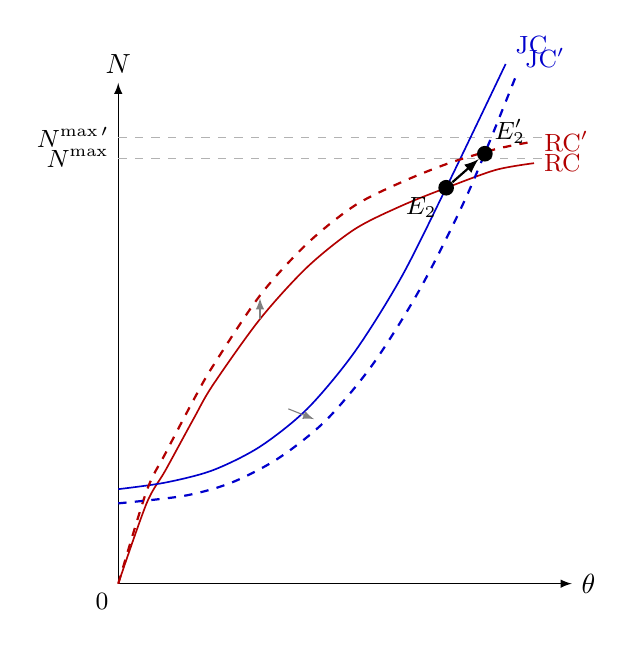
\begin{tikzpicture}[>=latex, scale=1.2,
		jc/.style={blue!80!black, semithick},
		rc/.style={red!70!black, semithick},
		jcp/.style={blue!80!black, thick, dashed},
		rcp/.style={red!70!black, thick, dashed},
		eqdot/.style={circle, fill=black, inner sep=2pt}]
		
		\draw[->] (0,0) -- (4.8,0) node[right] {$\theta$};
		\draw[->] (0,0) -- (0,5.3) node[above] {$N$};
		\node[below left, font=\small] at (0,0) {$0$};
		
		\draw[gray!60, thin, dashed] (0,4.5)
		node[left, font=\small, black] {$N^{\max}$} -- (4.5,4.5);
		\draw[gray!60, thin, dashed] (0,4.72)
		node[left, font=\small, black] {$N^{\max\prime}$} -- (4.5,4.72);
		
		\draw[rc] plot[smooth, tension=0.5] coordinates {
			(0,0)(0.3,0.85)(0.5,1.2)(0.8,1.75)
			(1.0,2.1)(1.5,2.8)(2.0,3.35)(2.5,3.75)
			(3.0,4.0)(3.5,4.2)(4.0,4.38)(4.4,4.45)
		} node[right, font=\small, red!70!black] {RC};
		
		\draw[jc] plot[smooth, tension=0.5] coordinates {
			(0,1.0)(0.5,1.07)(1.0,1.2)(1.5,1.45)
			(2.0,1.85)(2.5,2.45)(3.0,3.25)(3.5,4.25)(4.1,5.5)
		} node[above right, font=\small, blue!80!black] {JC};
		
		\draw[rcp] plot[smooth, tension=0.5] coordinates {
			(0,0)(0.3,0.98)(0.5,1.38)(0.8,1.95)
			(1.0,2.30)(1.5,3.05)(2.0,3.60)(2.5,4.00)
			(3.0,4.25)(3.5,4.45)(4.0,4.60)(4.4,4.68)
		} node[right, font=\small, red!70!black] {RC$'$};
		
		\draw[jcp] plot[smooth, tension=0.5] coordinates {
			(0,0.85)(0.7,0.93)(1.2,1.07)(1.7,1.33)
			(2.2,1.73)(2.7,2.33)(3.2,3.13)(3.7,4.13)(4.2,5.35)
		} node[above right, font=\small, blue!80!black] {JC$'$};
		
		\node[eqdot] at (3.47,4.19) {};
		\node[below left, font=\small] at (3.47,4.19) {$E_2$};
		
		\node[eqdot] at (3.88,4.55) {};
		\node[above right, font=\small] at (3.88,4.55) {$E_2'$};
		
		\draw[->, thick, shorten >=3pt, shorten <=3pt]
		(3.47,4.19) -- (3.88,4.55);
		
		\draw[->, gray, thin, shorten >=1pt]
		(1.8,1.85) -- (2.1,1.73);
		\draw[->, gray, thin, shorten >=1pt]
		(1.5,2.8) -- (1.5,3.05);
		
	\end{tikzpicture}
	\caption{Steady-state curves before (solid: JC, RC) and after (dashed: JC$'$, RC$'$) a
		permanent rise in $z$, with upper bounds $N^{\max}$ and $N^{\max\prime}$ and high
		equilibria $E_2$ and $E_2'$. Schematic.}
	\label{fig:steady_state_curves_z}
\end{figure}


	

	%%%%%%%%%%%%%%%%%%%%%%%%%%%%%%%%%%%%%%%%%
	\section{Empirical Evidence and Bartik Local Projections}\label{sec:empirical}
	%%%%%%%%%%%%%%%%%%%%%%%%%%%%%%%%%%%%%%%%%%

	\subsection{Overview and identification strategy}\label{sec:empirical_overview}

	The cross-state evidence in Section \ref{sec:introduction} establishes
	that states with structurally higher establishment exit rates accumulate
	larger unemployment gaps during recessions, but the correlation conflates
	the causal effect of exit shocks with persistent differences in industrial
	composition, institutional environment, and average firm age across
	states.  A state panel regression of labor market outcomes on local exit
	rates would confound the structural $\delta$ shock with the local demand
	conditions that drive both exits and unemployment simultaneously --- the
	classic omitted variable in any cross-sectional or within-state
	identification strategy.  The standard panel remedy of adding state and
	time fixed effects absorbs permanent cross-state heterogeneity and
	aggregate time variation but leaves untouched the within-state,
	within-time comovement between local exit activity and local business
	conditions.

	We address this using a Bartik shift-share design
	\citep{bartik_1991,goldsmith_2020}.  The instrument for state $i$ at
	quarter $t$ is a weighted average of \emph{national} industry-level
	establishment exit rates, where the weights are the state's
	pre-determined industry employment shares.  To see why this breaks the
	confound, consider Michigan in 2008: its instrument is large because
	manufacturing nationally --- not just in Michigan --- was experiencing
	a wave of permanent closings, and Michigan had a high pre-recession
	exposure to manufacturing.  The national exit rate is computed leaving
	out Michigan's own establishments (leave-one-out), so the instrument
	cannot be mechanically driven by Michigan-specific conditions.  The
	instrument thus isolates variation in exit exposure driven by a
	state's inherited industry structure interacting with national industry
	cycles, rather than by local demand or policy.

	The identifying assumption is that, conditional on state and time fixed
	effects and lagged controls, the Bartik instrument is uncorrelated with
	state-specific shocks to unemployment and vacancy creation beyond the
	exit channel. Section~\ref{sec:empirical_instr}
	describes instrument construction in detail;
	Section \ref{sec:empirical_lp} states the local projection
	specification; Section~\ref{sec:empirical_results} reports results. Section~\ref{sec:empirical_results} provides two
	validation exercises: a severity placebo that tests whether the vacancy
	IRF is driven by recession depth rather than exit exposure, and a joint
	local projection that checks robustness to controlling simultaneously
	for the layoff-and-discharge instrument.  

	\subsection{Instrument construction}\label{sec:empirical_instr}

	\paragraph{BED data and the permanence problem}
	The underlying data source is the BLS Business Employment Dynamics
	(BED) survey, which tracks establishment-level employment via state
	unemployment insurance payroll records at quarterly frequency from
	1992Q3.  BED dates each establishment by third-month employment.  An
	establishment is classified as a ``closing'' in a given quarter if it
	reported positive employment in the third month of the previous
	quarter and reports zero employment in the third month of the current
	quarter.  Coverage is all private-sector establishments across
	12 supersectors and all 50 states.

	Raw BED closings conflate two economically distinct events:
	\emph{permanent exits} --- establishments that dissolve irreversibly,
	destroying the associated product line and vacancy slot --- and
	\emph{temporary shutdowns}, establishments that suspend operations for
	one to three quarters before reopening.  The model's $\delta$ shock
	corresponds exclusively to permanent exit: only an irreversible
	dissolution removes a product line from the variety space and
	eliminates the recruiter's vacancy.  Using raw closings as the shock
	proxy therefore overstates the true destruction margin and introduces
	attenuation bias when the temporary-shutdown share varies over time.
	The contamination is most severe during the 2020Q2 lockdown, where
	roughly 400,000 of the recorded closings reflected government-mandated
	suspensions that subsequently reopened, but it is present at lower
	intensity throughout the sample: seasonal businesses, firms temporarily
	suspending operations during downturns, and establishments undergoing
	ownership transitions all appear as closings in BED without
	constituting permanent product-line destruction.

	\paragraph{BED Deaths as the measure of permanent exits}
	We address this using a second BED data series that resolves the
	permanence problem directly.  In addition to closings, BED separately
	reports \emph{deaths}, which by construction exclude temporary
	shutdowns.  Let $q_0$ denote the last quarter in which an
	establishment reports positive third-month employment.  The
	establishment is a closing in $q_0+1$.  It is a \emph{death} only if
	it reports zero employment in the third month of each of the four
	consecutive quarters $q_0+1$ through $q_0+4$.  A death is therefore a
	closing that is followed by three further quarters of confirmed zero
	employment.\footnote{BED data classes: 06 (Closings) and 08 (Deaths).
	Deaths $\subseteq$ Closings in every industry$\times$quarter cell, so
	the ratio is bounded above by unity by construction.}  Since a
	temporarily closed establishment re-enters the payroll base within one
	to three quarters, it never accumulates four consecutive zero
	quarters and therefore never appears in BED Deaths.  Our $\delta$
	instrument uses BED Deaths, not raw closings, as the numerator of the
	national exit rate.

	Two features of this definition matter for the empirical design.
	First, the four-quarter rule is a \emph{confirmation} requirement, not
	a dating rule.  BLS attributes the death to the quarter in which the
	establishment closed, so the series is correctly timed even though it
	can only be finalized four quarters later.  The rule induces a
	publication lag and vintage revisions.  It does not shift the
	destruction series forward in time, and so cannot by itself generate
	delayed dynamics in the local projections of
	Section~\ref{sec:empirical_results}.  Second, the criterion is
	stricter than the annual Census Business Dynamics Statistics (BDS)
	measure of establishment deaths, which compares employment in the
	first quarter of consecutive years and therefore still counts an
	establishment that is idle at the reference date but later reopens.
	BED Deaths applies the spirit of the BDS permanence screen at
	quarterly frequency, with a tighter permanence criterion.

	Figure~\ref{fig:bed_deaths} shows employment-weighted mean BED Closings
	and Deaths rates across 12 supersectors from 1992Q3 to 2019Q4, together
	with 10th--90th industry percentile bands.  The Deaths/Closings ratio
	(lower panel) averages 0.63 across the full sample and is remarkably
	stable over the business cycle, dipping modestly during the GFC but
	remaining well below unity throughout.  This stability implies that the
	fraction of closings that are temporary does not vary sharply over time,
	and that using Deaths directly gives a cleaner series than either raw
	closings or a time-varying permanence correction.

	\begin{figure}[h]
		\centering
		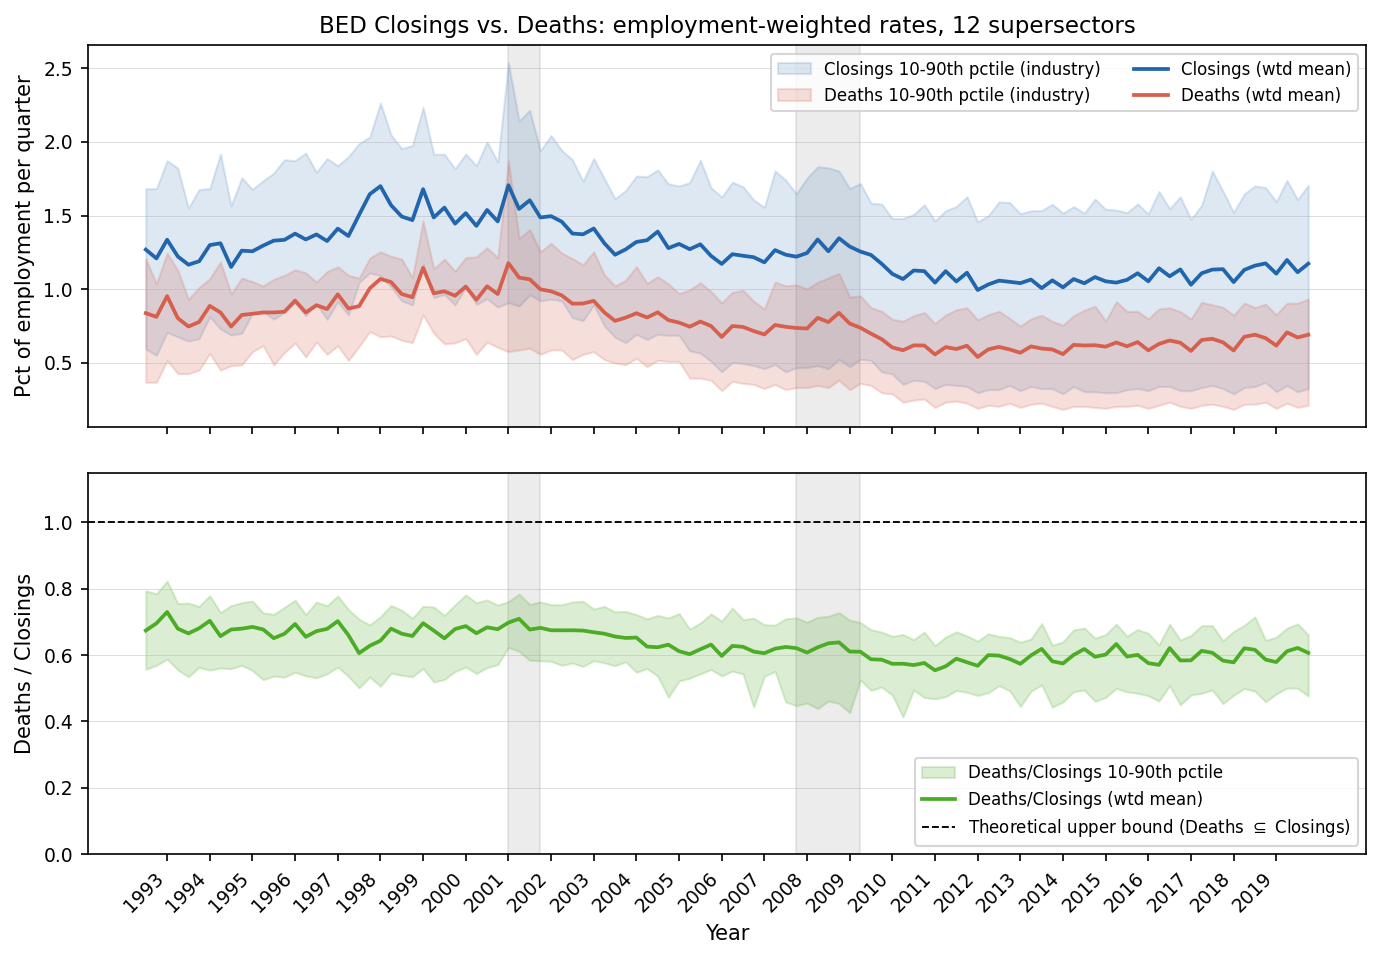
\includegraphics[width=\linewidth]{bed_closings_vs_deaths.png}
		\caption{BED Closings and Deaths: employment-weighted rates across
		12 supersectors, 1992Q3--2019Q4.  \emph{Top panel:} mean closing
		rate (blue) and death rate (red) as percent of employment per
		quarter, with 10th--90th industry percentile bands.  Grey shading
		denotes NBER recessions.  \emph{Bottom panel:} Deaths/Closings
		ratio (dashed line at 1.0 marks the theoretical upper bound;
		ratio is bounded above by unity since Deaths $\subseteq$ Closings
		in every industry$\times$quarter cell).}
		\label{fig:bed_deaths}
	\end{figure}

	The Deaths/Closings ratio exhibits substantial cross-sector
	heterogeneity.  Mining has the lowest mean ratio (0.37), and
	Construction is similarly low (0.52), consistent with the prevalence
	of project-based and seasonal establishments that suspend operations
	temporarily without constituting permanent product-line destruction.
	Leisure and hospitality (0.58) and Other services (0.59) are also
	below the sample average.  At the other end, Manufacturing (0.71),
	Retail trade (0.70), and Information (0.70) have the highest ratios,
	reflecting structurally lower rates of temporary closure in those
	sectors.  No supersector reaches the theoretical upper bound of unity
	in any quarter of the sample.  The employment-weighted mean across all
	12 supersectors is 0.63 (2001--2019); supersector time series are
	shown in ~\ref{app:deaths_closings_supersector}.

	Most papers using BED data for shock identification
	\citep[e.g.,][]{elsby_2013} implicitly treat all
	closings as permanent.  We are not aware of a prior paper using the
	BED Deaths series to align the instrument with the structural concept
	of irreversible product-line destruction.

	\paragraph{Leave-one-out construction and base-year shares}
	The leave-one-out (LOO) national permanent exit rate for state $i$,
	supersector $j$, quarter $t$ is
	\begin{equation}\label{eq:loo_rate}
		g^{\delta}_{-i,j,t}
		\;=\;
		\frac{\text{deaths}_{j,t}}
		     {E^{\text{nat}}_{-i,j,t_0}},
	\end{equation}
	where $E^{\text{nat}}_{-i,j,t_0}=E^{\text{nat}}_{j,t_0}-E_{i,j,t_0}$
	is base-year national employment in supersector $j$ minus state $i$'s
	own base-year employment.  The LOO correction in the denominator
	ensures that state $i$'s own exit activity cannot mechanically inflate
	its instrument value.  Numerator LOO --- subtracting state $i$'s own
	deaths from the national count --- is not implemented because
	BED state-level deaths by supersector are not publicly available.  Employment shares $\omega_{i,j}$ are drawn from the 2006
	QCEW (agglvl=54, private sector), a stable pre-GFC year that predates
	the bulk of the identifying variation.  The Bartik instrument is:
	\begin{equation}\label{eq:bartik_delta}
		B^{\delta}_{i,t}
		\;=\;
		\sum_{j} \omega_{i,j}\cdot g^{\delta}_{-i,j,t}.
	\end{equation}

	\paragraph{Residualization}
	Raw BED exit rates co-move with industry-specific demand conditions:
	when a sector contracts nationally, establishments exit at higher rates
	\emph{and} surviving firms simultaneously reduce vacancy posting and
	raise layoffs.  An instrument built on raw $g^\delta_{j,t}$ would
	therefore partly identify the effect of industry demand contractions
	rather than the structural $\delta$ shock.  We address this by
	projecting each log shock rate on predetermined demand controls before
	Bartik aggregation, retaining the residual as the instrument input.

	The baseline residualization (v2) runs a within-industry OLS regression:
	\begin{equation}\label{eq:resid_v2}
		\log g^{\delta}_{j,t}
		\;=\;
		\alpha_j + \gamma\,\Delta\!\log p_t
		         + \lambda\,\Delta\!\log VA_{j,t-1}
		         + \nu^{\delta}_{j,t},
	\end{equation}
	where $\Delta\!\log p_t$ is aggregate nonfarm business productivity
	growth (FRED: OPHNFB) and $\Delta\!\log VA_{j,t-1}$ is real
	value-added growth in supersector $j$ lagged one quarter (BEA via
	FRED series RVAM, RVAC, etc.).  Both regressors are predetermined
	relative to the current-period shock draw: aggregate productivity is
	contemporaneous but common to all industries and thus absorbed by the
	time fixed effects in the second stage; industry VA is lagged one
	quarter to ensure strict predetermination.  The residual
	$\nu^{\delta}_{j,t}$ is then Bartik-aggregated in place of the raw
	rate, yielding $\tilde{B}^{\delta}_{i,t}$.

	The FRED BEA real value-added series begin in 2005Q1, which would
	restrict the $\delta$ residualization sample to 2005Q2.  To recover
	the full 1997Q1+ sample, we extend the quarterly VA series back to
	1992Q1 using a constrained Chow-Lin (1971) temporal disaggregation.
	An indicator regression estimated on the 2005Q1+ post-sample relates
	quarterly sectoral VA growth to real GDP growth:
	$\Delta\!\log VA_{j,t}=\alpha_j+\beta_j\,\Delta\!\log\text{GDP}_t+\varepsilon_{j,t}$.
	The pre-2005 quarterly path is recovered by applying the implied
	growth rates $\hat{\alpha}_j+\hat{\beta}_j\,\Delta\!\log\text{GDP}_t$
	recursively from the 2005Q1 anchor level.  The backcast is then
	constrained to match published BEA annual benchmarks for 1997--2004
	via a proportional Denton adjustment: for each year $A$ with annual
	benchmark $Y_{j,A}$, quarterly values are scaled by
	$Y_{j,A}/\overline{VA}_{j,A}^{\text{unconstrained}}$ so that the
	within-year average equals the published figure exactly.  Industries
	with low GDP--VA correlation (R$^2$ below threshold) receive
	$\hat{\beta}_j=0$, using only the sector-specific mean growth rate to
	avoid injecting noisy cyclical variation into the pre-period.

	After v2 residualization the cross-state correlation between the
	$\delta$ and layoffs-and-discharges (LD) Bartik instruments falls from
	approximately 0.54 on raw rates to 0.33.\footnote{As a robustness check we further augment equation~\eqref{eq:resid_v2}
		with a monetary policy sensitivity term
		$\psi(\phi_j\times\Delta MP_t)$, where $\phi_j$ is log average
		establishment size in supersector $j$ (Census CBP, 2000) and
		$\Delta MP_t$ is the quarterly change in the Wu--Xia (2016) shadow
		federal funds rate (v3 specification).  The v3 results are reported
		in \ref{app:robustness}; v2 is the baseline throughout.}  The persistence of this residual correlation after
	controlling for industry demand cycles and aggregate productivity is
	informative: the shared variation is not a demand artifact but most
	likely reflects industry-specific financial conditions that move both
	exit rates and layoff rates simultaneously.  This motivates the joint
	local projection robustness check in
	Section~\ref{sec:empirical_results}.

	\begin{figure}[H]
		\centering
		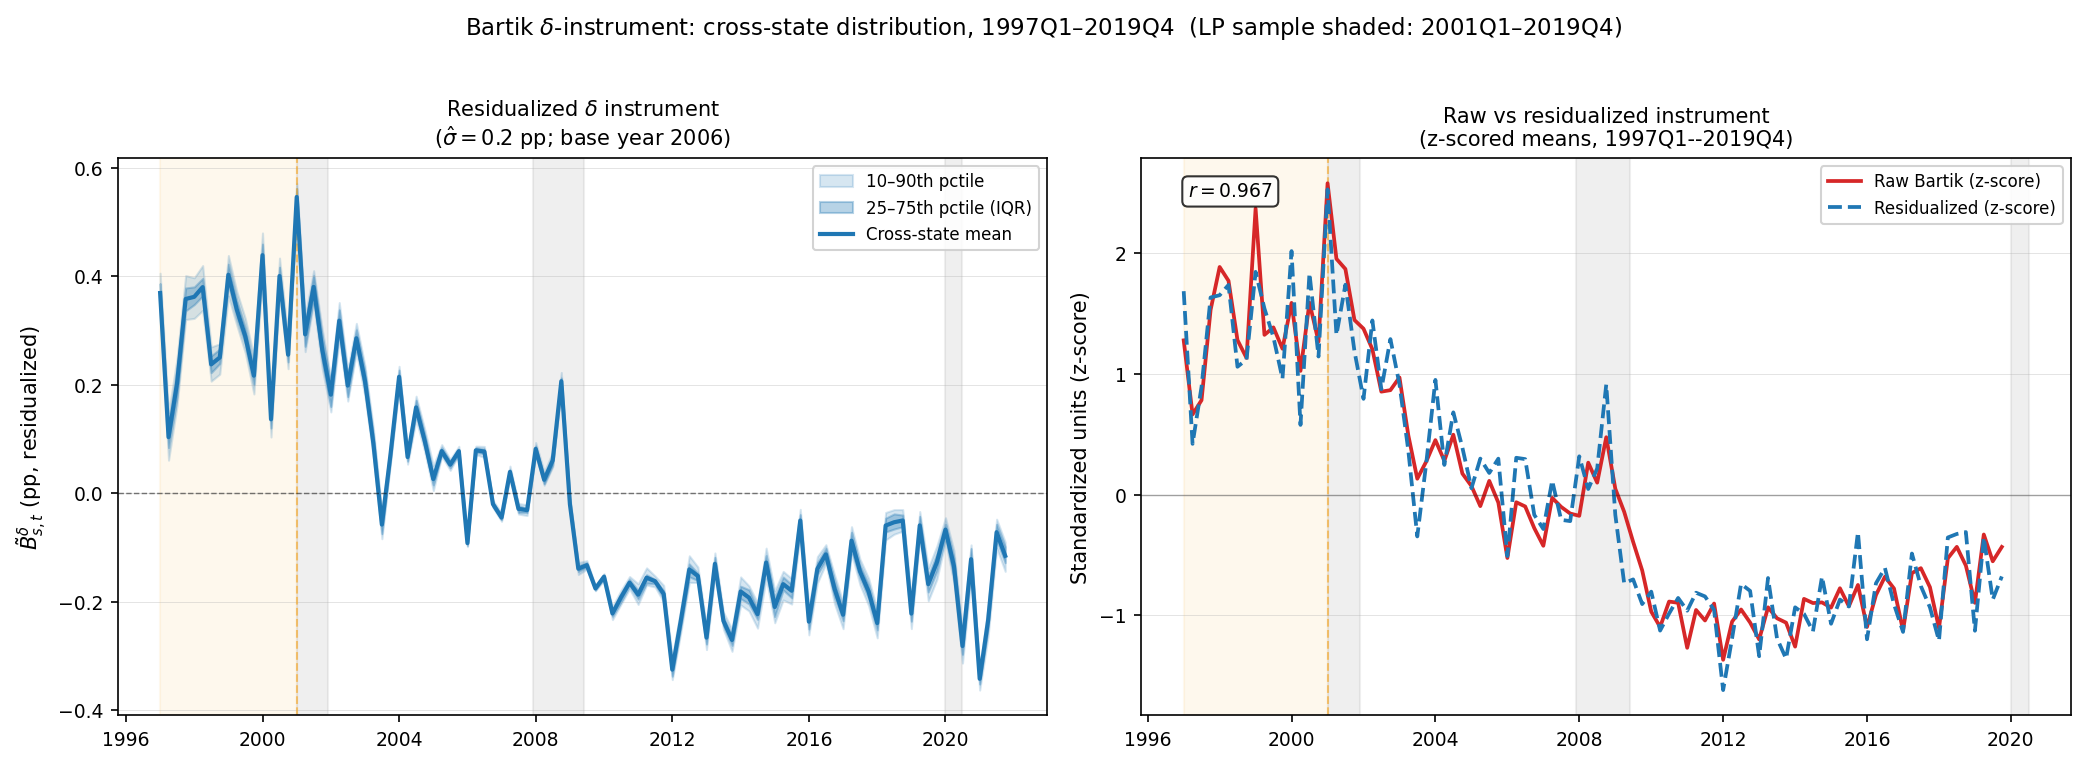
\includegraphics[width=\linewidth]{instrument_delta_distribution.png}
		\caption{Cross-state $\delta$ Bartik instrument distribution,
			1997Q1--2019Q4.
			\emph{Left:} residualized instrument $\tilde{B}^{\delta}_{i,t}$
			(pp of base-year employment); shading shows 25th--75th (dark) and
			10th--90th (light) cross-state percentile bands.
			\emph{Right:} z-scored cross-state means of raw (red) and
			residualized (blue dashed) instruments; $r = 0.905$.
			Orange shading (1997Q1--2000Q4): pre-LP period available for
			$\delta\to u$ but not vacancy or LD/QU.
			Grey shading: NBER recessions.}
		\label{fig:delta_distribution}
	\end{figure}

	Figure~\ref{fig:delta_distribution} documents the cross-state
	distribution of the instrument and the effect of residualization.
	Both panels extend to 1997Q1, the start of the Chow--Lin-extended
	value-added series; the orange-shaded region (1997Q1--2000Q4) marks
	the pre-JOLTS period that is available for the $\delta\to u$
	specification but not for the vacancy LP.
	The left panel shows substantial cross-sectional dispersion
	throughout, with the interquartile range widening sharply during the
	GFC.  Negative values in some states and quarters reflect
	lower-than-predicted closing rates given prevailing aggregate
	conditions and industry composition; since the local projection
	absorbs the cross-state mean via time fixed effects, identification
	comes from cross-sectional variation in residualized exposure, which
	remains well-defined regardless of sign.

	The right panel compares the z-scored cross-state means of the raw
	and residualized instruments ($r = 0.905$).  The two series track
	each other closely throughout the sample, indicating that
	residualization does not materially alter identifying variation in
	normal times.  Two episodes diverge.  During the GFC, the
	residualized mean rises somewhat more than the raw instrument at
	2008Q4 ($z = 1.51$ vs.\ $0.95$), consistent with residualization
	removing attenuating aggregate and industry-level variation.  The
	more striking divergence would appear in 2020Q2 (not shown, excluded
	from LP sample): the raw Bartik spikes to $z = 2.33$ while the
	residualized instrument falls to $z = -0.45$, because 2020Q2 BED
	closings were dominated by government-mandated temporary shutdowns
	that correlate strongly with industry composition and aggregate
	conditions; residualization correctly removes this variation, leaving
	below-average permanent destruction.  This episode illustrates
	precisely why the LP sample is capped at 2019Q4.

	The cross-state mean of the instrument exhibits a pronounced secular
	decline over the sample, falling roughly one-third from the late
	1990s to the late 2010s.  This mirrors the well-documented decline in
	aggregate labor market fluidity: the \citet{shimer_2005} quarterly
	separation rate fell proportionally over the same period, and the
	ratio of the two series is nearly constant throughout (coefficient of
	variation 14\%), indicating that permanent establishment destruction
	has declined in tandem with broader separation margins rather than
	becoming relatively more or less important over time.

	Two features of the left panel deserve note.  First, the
	cross-sectional percentile bands are narrow relative to the
	time-series movement of the mean: the within-quarter p90--p10 spread
	averages 0.045\,pp, a coefficient of variation of about 15\%.  The
	pooled standard deviation across all state-quarters ($\hat{\sigma} =
	17.4$\,pp) is therefore predominantly a time-series number, reflecting
	the common component of the instrument that moves all states together.
	The time fixed effects in the local projection absorb this common
	component; identification comes from the within-period cross-sectional
	deviations, which have a typical magnitude of roughly 0.02\,pp.
	Second, some state-quarter cells take negative values, reflecting
	lower-than-predicted closing rates given industry composition and
	aggregate conditions; these are well-defined as deviations from the
	cross-state mean and cause no identification problem.

	\subsection{Local projection specification}\label{sec:empirical_lp}

	For each horizon $h=0,1,\ldots,20$ quarters, the panel local projection
	estimating equation is
	\begin{equation}\label{eq:lp}
		y_{i,t+h} - y_{i,t-1}
		\;=\;
		\alpha_i + \alpha_t
		+ \beta_h\,\tilde{B}^{\delta}_{i,t}
		+ \gamma_1\,y_{i,t-1}
		+ \gamma_2\,\log L_{i,t-1}
		+ \varepsilon_{i,t+h},
	\end{equation}
	where $y_{i,t}$ is the labor market outcome of interest for state $i$ in quarter $t$,
	$\tilde{B}^{\delta}_{i,t}$ is the residualized $\delta$ Bartik instrument
	constructed in Section~\ref{sec:empirical_instr}, $\alpha_i$ and
	$\alpha_t$ are state and time fixed effects, $y_{i,t-1}$ is the lagged
	outcome, and $L_{i,t-1}$ is the lagged labor force.  The left-hand side
	measures the cumulative $h$-period change relative to the quarter before
	the shock, so the sequence $\{\hat\beta_h\}$ traces the impulse response
	directly.  Standard errors are clustered at the state level ($n=50$).

	The two outcomes are the state unemployment rate $u_{i,t}$ and vacancy
	rate $v_{i,t}$, both in percentage points (unemployed persons or
	vacancies as a share of the labor force).  Concretely,
	$v_{i,t} = 100 \times V_{i,t}/L_{i,t}$, where $V_{i,t}$ is the
	quarterly average of monthly JOLTS job-openings stocks (seasonally
	adjusted) and $L_{i,t}$ is the LAUS labor force.  The two
	specifications differ only in the autoregressive control $y_{i,t-1}$.

	The estimation sample runs from 2001Q1, when JOLTS state vacancy data
	become available, through 2019Q4; observations with $t+h >
	\text{2019Q4}$ are dropped to exclude COVID-19.\footnote{The $\delta$
		unemployment equation can be estimated back to 1997Q1 using the
		Barnichon (2010) Composite Help-Wanted Index as a pre-JOLTS vacancy
		proxy; extending the sample attenuates the IRF modestly (peak
		$+1.07$ pp vs.\ $+1.50$ pp) because the 1997--2000 expansion years
		exhibit faster reabsorption of displaced workers.  We use the 2001Q1
		baseline throughout to maintain a common sample across both outcomes.}
	The instrument $\tilde{B}^{\delta}_{i,t}$ has cross-sectional standard
	deviation $\hat\sigma_{\tilde{B}^\delta} = 17.4$ pp; all reported
	$\hat\beta_h$ are scaled by $\hat\sigma_{\tilde{B}^\delta}^{-1}$ so
	that the impulse responses correspond to a one-standard-deviation shock.

	We also construct Bartik instruments for layoffs-and-discharges
	$\tilde{B}^{\text{LD}}$ (JOLTS LD) and quits $\tilde{B}^{\text{QU}}$
	(JOLTS quits), using the same 2006 QCEW base-year shares and v2
	residualization.  Neither is treated as a well-identified separate
	estimation target.  $\tilde{B}^{\text{LD}}$ conflates genuine match
	dissolution at surviving establishments with vacancy withdrawals at
	partially closing firms, mixing $s$- and $\delta$-type events in
	proportions that vary across industries and cycles; moreover,
	$\tilde{B}^{\delta}$ Granger-causes future LD through $h=12$ while the
	reverse predictability fades by $h=8$, indicating that LD is partly
	endogenous to destruction.  $\tilde{B}^{\text{QU}}$ is procyclical and
	driven largely by job-to-job transitions, which represent a worker gain
	for one employer offset by a hire at another and have no clear mapping
	to the model's match separation shock $s$; we include it as a diagnostic
	instrument only.\footnote{In particular, a high quit rate in an industry
	does not imply that vacancies go unfilled --- the quitting worker is
	typically replaced by a job-to-job mover from elsewhere, so the net
	effect on aggregate vacancies is near zero.  This is conceptually
	distinct from the $s$ shock in the model, which destroys a match and
	triggers a vacancy repost.}  Both instruments and their local
	projections are reported in \ref{app:diagnostics}.

	\begin{figure}[H]
		\centering
		\includegraphics[width=0.92\textwidth]{lp_irf_delta_uv_baseline.png}
		\caption{Impulse responses of the state unemployment rate (left)
			and vacancy rate (right) to a one-standard-deviation increase
			in the residualised $\delta$ Bartik instrument
			($\hat{\sigma}_{\tilde{B}^\delta}=17.4$ pp, 2001Q1--2019Q4).
			Both outcomes are estimated from panel local projections with
			state and time fixed effects; standard errors are clustered at the
			state level ($n=50$).  Shaded band: 90\% confidence interval;
			dashed lines: 95\% confidence interval.  The instrument is
			BED establishment deaths (equation~\eqref{eq:bartik_delta}),
			residualized on aggregate productivity growth and lagged industry
			value-added growth (equation~\eqref{eq:resid_v2})}
		\label{fig:delta_uv_irf}
	\end{figure}

	\subsection{Results}\label{sec:empirical_results}

	% --- delta -> u and delta -> v IRFs ---

	Figure~\ref{fig:delta_uv_irf} reports the impulse responses of the
	state unemployment rate and vacancy rate to a one-standard-deviation
	increase in the residualized $\delta$ Bartik instrument
	($\hat{\sigma}_{\tilde{B}^\delta} = 17.4$ pp, 2001Q1--2019Q4 sample).
	The unemployment response rises steadily from $0.22$ pp at $h=0$ to
	a plateau of $+1.71$ pp by $h=17$--$20$, remaining highly significant
	throughout ($p < 0.001$ from $h=0$).  The vacancy response falls
	persistently from $-0.11$ pp at $h=0$ to a trough of $-0.58$ pp at
	$h=18$, significant at $p < 0.01$ from $h=2$ onward and remaining so
	through $h=20$.  The simultaneous and persistent rise in unemployment
	alongside the fall in vacancies traces the outward leg of a Beveridge
	loop, consistent with the model's central prediction that permanent
	product-line destruction depletes the vacancy stock rather than merely
	suspending it.

	A notable feature of the two IRFs is their asymmetric dynamics at
	medium horizons: the vacancy response stabilizes around $h = 12$--$14$
	while the unemployment response continues to rise through $h = 20$.
	This pattern is consistent with a recovery path in which new vacancy
	creation resumes before the unemployment pool fully clears.  Whether the
	calibrated model replicates this relative timing is testable and will
	be assessed in Section~\ref{sec:quantitative}.

	% --- Severity placebo ---

	A natural concern is that the $\delta$ Bartik instrument may inadvertently
	capture recession severity: states with structurally high establishment turnover
	may also experience worse aggregate downturns, so the IRF could reflect
	demand-driven labor-market deterioration rather than product-line destruction
	per se.  We address this with a severity placebo that augments the baseline
	local projection with two interactions: $\tilde{B}_t^\delta \times
	\bar{u}_t^{\text{nat}}$, a level proxy for underlying economic slack, and
	$\tilde{B}_t^\delta \times \Delta\bar{u}_t^{\text{nat}}$, a flow proxy for
	cyclical momentum.  If the instrument were a severity proxy, these interactions
	should absorb the baseline IRF.  Instead, both interaction coefficients are
	insignificant at every horizon $h = 0, \ldots, 20$ for the vacancy outcome, and
	the baseline $\delta \to v$ coefficients are unchanged in magnitude and
	significance.  This is the cleanest external validity check in the paper: the
	vacancy response to establishment destruction is not explained by where
	the aggregate economy happens to stand in the cycle.  The severity placebo
	also passes for the unemployment outcome, though the interpretation is less
	sharp given the natural correlation between any adverse state-level shock and
	local unemployment.  Robustness results for the alternative instruments and
	the joint local projection are collected in
\ref{app:diagnostics}.

	%%%%%%%%%%%%%%%%%%%%%%%%%%%%%%%%%%%%%%%%%%
	\section{Quantitative analysis}\label{sec:quantitative}
	\subsection{Relationship to Coles and Kelishomi}\label{sec:ck_comparison}

	Our framework nests \citet{coles_2018} as a special case, as formalized in
	Proposition~\ref{prop:double_limit} and Remark~\ref{rem:nesting}. Relative to their calibration, we make two
	departures. First, we set $\delta$ to the BED Deaths employment-weighted exit rate
	($\bar\delta \approx 1.1\%$ per quarter) rather than equating it to the full
	aggregate separation rate; \citet{gabrovski_2025} show this correction materially
	improves the model's fit on the unemployment--productivity correlation. Second, we
	expand the estimation moment set to include the permanent exit rate $\delta$ and
	the entry flow $N^e_t$ (proxied by BFS high-propensity business applications), and supplement unconditional second moments with
	identified IRFs from the Bartik local projections of Section~\ref{sec:empirical}
	to separately discipline the propagation dynamics of $\delta$ and $s$ shocks.

	\subsection{Calibration and estimation}\label{sec:calib}

	This section sets out our estimation and calibration strategy, the taxonomy of
	parameters, and the explicit mapping from empirical targets to model objects.

	\medskip\noindent\textbf{Estimation framework.}
	We estimate the model by Bayesian simulated method of moments, combining two
	complementary sets of moment conditions that together over-identify the parameter
	vector.

	The first set consists of unconditional second moments of HP-filtered aggregate
	time series, extending \citet{coles_2018}. We target three groups: (i)~standard
	deviations ($m_1$), (ii)~contemporaneous pairwise correlations ($m_2$), and
	(iii)~first-order autocorrelations ($m_3$) for unemployment, vacancies,
	separations, the job-finding rate, the permanent exit rate, business
	applications, and labor productivity. The full empirical moment matrix is
	reported in Table~\ref{tab:smm_moments}. All series are log-transformed and
	HP-filtered with smoothing parameter $\lambda = 1{,}600$ before computing
	moments; the identical filter is applied to simulated model data when evaluating
	$m(\theta)$. This symmetric treatment renders HP-filtered second moments a valid
	indirect inference target: \citet{canova_2011} establish that applying
	the same filter to data and simulated output controls for any filter-induced
	distortion, even when the filter introduces spurious dynamics in isolation.
	We prefer $\lambda=1{,}600$ over the $\lambda=100{,}000$ convention of
	\citet{coles_2018} because the higher smoothing parameter strips out the
	business-cycle frequency variation in $\delta$ at which the destruction
	mechanism operates, reversing the sign of $\text{cor}(\delta,v)$ and driving
	$\text{cor}(\delta,u)$ to near zero --- an artifact of over-smoothing rather
	than a feature of the data.  \ref{app:filter_robustness} documents
	this explicitly: across the Hamilton (2018) regression filter, first differences,
	and HP with $\lambda=1{,}600$, the correlations $\text{cor}(\delta,u)>0$ and
	$\text{cor}(\delta,v)<0$ are robust; $\lambda=100{,}000$ is the anomalous
	specification.

\begin{table}[H]
\centering
\begin{threeparttable}
\caption{Business Cycle Moments}
\label{tab:smm_moments}
\begin{tabular}{l r @{\hspace{6pt}\vline\hspace{6pt}} r r r r r r r @{\hspace{6pt}\vline\hspace{6pt}} r}
\toprule
  &  $\sigma(x)$  &  \multicolumn{7}{c}{Contemporaneous correlations}  &  $\rho_1(x)$  \\
\cmidrule(lr){3-9}
  &  &  $u$  &  $v$  &  $\tau$  &  $f$  &  $\delta$  &  $N^e$  &  $z$  &  \\
\midrule
  Unemployment  &  0.1496  &  $1$  &    &    &    &    &    &    &  0.792  \\
  Vacancies  &  0.1419  &  -0.804  &  $1$  &    &    &    &    &    &  0.902  \\
  Separations  &  0.1019  &  0.577  &  -0.422  &  $1$  &    &    &    &    &  0.250  \\
  Job-finding rate  &  0.0977  &  -0.791  &  0.620  &  0.020  &  $1$  &    &    &    &  0.808  \\
  Exit rate  &  0.0793  &  0.310  &  -0.246  &  0.681  &  0.213  &  $1$  &    &    &  0.114  \\
  Entry flow ($N^e$)  &  0.0813  &  -0.105  &  0.482  &  -0.345  &  -0.226  &  -0.496  &  $1$  &    &  0.545  \\
  Labor productivity  &  0.0128  &  -0.009  &  0.306  &  -0.228  &  -0.212  &  -0.250  &  0.381  &  $1$  &  0.766  \\
\midrule
  \multicolumn{10}{l}{\textit{Derived statistics}}  \\
  \quad $\sigma(\theta)/\sigma(z)$  &  11.70  &    &    &    &    &    &    &    &    \\
\bottomrule
\end{tabular}
\begin{tablenotes}[flushleft]
\footnotesize
\item \textit{Note:} HP filter with $\lambda = 1{,}600$ applied to log-levels of each series. Correlations use pairwise-complete observations; the shortest series ($N^e$, entry flow) begins 2004Q3. Sources --- $u$: BLS LAUS; $v$: Barnichon (2010) composite HWI spliced with BLS JOLTS at 2001Q1; $s$, $f$: Shimer (2012) continuous-time flows from CPS; $\delta$: BLS BED Deaths (dataclass 08), employment-weighted; $N^e$: BFS high-propensity business applications (BAWBATOTALSAUS) per capita, proxy for model entry flow; $z$: BLS PRS85006163 (output per hour, nonfarm business).
\end{tablenotes}
\end{threeparttable}
\end{table}
Table~\ref{tab:smm_moments} highlights several salient features of the data.
Unemployment and vacancies are highly volatile relative to labor productivity
($\sigma(u)/\sigma(z) \approx 11.7$, $\sigma(v)/\sigma(z) \approx 11.1$) and
display a pronounced Beveridge curve ($\text{cor}(u,v)=-0.80$).  The
unemployment-labor productivity correlation is near zero ($\text{cor}(u,z)=-0.01$),
consistent with weak technology-shock transmission in models with endogenous
separation.  The exit rate co-moves strongly with the match separation rate
($\text{cor}(\delta,\tau)=0.68$), reflecting a common cyclical component of firm
destruction and worker-job dissolution.  Importantly, the exit rate is positively
correlated with unemployment ($\text{cor}(\delta,u)=0.31$) and negatively correlated
with vacancies ($\text{cor}(\delta,v)=-0.25$), consistent with the simultaneous
vacancy-destruction mechanism central to our model.\footnote{These signs reverse under
$\lambda=10^5$, an artifact of over-smoothing
documented in\ref{app:filter_robustness}.}  Labor market variables and
entry display strong persistence ($\rho_1 \in [0.55, 0.90]$), while separations
and the exit rate exhibit substantially less ($\rho_1 \approx 0.11$--$0.25$),
consistent with their role as shock-propagation mechanisms rather than persistent states.


The second set consists of empirically identified impulse responses from the
	Bartik local projections of Section~\ref{sec:empirical}: the $h=0,\ldots,H$
	quarter paths of unemployment and vacancies following a one-standard-deviation
	$\delta$ shock. Following \citet{christiano_2016}, we form a Gaussian
	quasi-likelihood based on the sampling distribution of the LP estimator:
	\begin{align}\label{eq:ql_irf}
		\log \mathcal{L}_{\mathrm{IRF}}(\theta)
		= -\tfrac{1}{2}(\hat\beta - \beta(\theta))'\Omega_\beta^{-1}(\hat\beta -
		\beta(\theta)),
	\end{align}
	where $\hat\beta$ stacks the two estimated IRF paths, $\beta(\theta)$ is the
	corresponding model-implied path computed from the linearized state-space
	representation, and $\Omega_\beta$ is the sampling covariance estimated by wild
	cluster bootstrap with $n=50$ state clusters.

	The quasi-likelihood is a limited-information Bayesian update: rather than
	conditioning on the raw panel data, it conditions on $\hat\beta$ as a sufficient
	statistic for the model-implied path $\beta(\theta)$. 
	Writing the full likelihood $\mathcal{L}(\mathrm{data}|\theta)$ for the panel
	would require the model to generate 50 state-level employment series, cross-state
	variation in industry composition, and the full Bartik instrument---objects entirely
	outside a representative-agent aggregate economy.  Even setting this aside, any
	reduced-form likelihood over $\hat\beta$ would require distributional assumptions
	on the LP residuals, the instrument's conditional distribution, and the
	finite-sample behavior of a clustered two-stage estimator---auxiliary assumptions
	with no grounding in the structural model.  The quasi-likelihood avoids both
	problems by relying only on the asymptotic normality of $\hat\beta$, which
	follows from the LP moment conditions alone \citep{chernozhukov_2003}.

	What is the value of using the IRF block instead of relying on the structural likelihood on aggregate time series? The answer is identification.  The full likelihood recovers structural
	parameters from the time-series covariance structure of observables, but in a
	three-shock model the unconditional second moments cannot separately discipline the
	propagation of $\delta$ and $s$ shocks: both raise unemployment, and their
	vacancy responses---the qualitative distinction between them---are collinear in
	second moments because they depend jointly on shock persistence, sunk-cost
	dynamics, and the entry margin.  The Bartik design provides the only clean
	exogenous variation in $\delta$ and therefore the only moment condition that
	separately identifies the parameters governing the model's central mechanism.
	Omitting the IRF block would leave the asymmetric vacancy-destruction channel
	weakly identified from time-series covariances alone.

	A filtering asymmetry between the two blocks is present by design: unconditional
	moments are statistics of HP-filtered data, while IRF coefficients are estimated
	from level regressions. This is resolved on the model side. Model moments
	$m(\theta)$ are computed from simulated-then-filtered data, mirroring the data
	construction. Model IRFs $\beta(\theta)$ are read directly from the state-space
	impulse response without filtering, mirroring the LP estimation. The two objects
	therefore target genuinely distinct features of the model---cyclical second-moment
	structure and shock-specific propagation dynamics---in a way that is internally
	consistent on both the data and model sides.

	The two blocks provide complementary identification. Unconditional moments
	discipline the level and cyclical volatility of the destruction and separation
	processes, the amplification and comovement structure, and the persistence of key
	aggregates. The IRF block separately identifies the dynamic transmission of
	$\delta$ shocks---in particular, the simultaneous elimination of vacancies that
	distinguishes $\delta$ from $s$ and generates persistent Beveridge-curve
	dislocations---identification unavailable from unconditional moments alone, which
	conflate the contributions of all three shocks.

	To prevent the IRF block from mechanically dominating the joint objective by
	virtue of moment count, we normalize each block's quadratic form by its
	dimension. Letting $K_\beta$ denote the number of IRF moment conditions and
	$K_m$ the number of unconditional moments, the log-posterior kernel is
	\begin{align}\label{eq:posterior}
		\log p(\theta \mid \mathrm{data})
		\propto \log\pi(\theta)
		- \frac{1}{2K_\beta}(\hat\beta - \beta(\theta))'\Omega_\beta^{-1}
		(\hat\beta - \beta(\theta))
		- \frac{1}{2K_m}(\hat m - m(\theta))'\Omega_m^{-1}(\hat m - m(\theta)),
	\end{align}
	where $\hat m$ collects the empirical moments from Table~\ref{tab:smm_moments},
	$m(\theta)$ the corresponding model-implied moments from simulated HP-filtered
	data, and $\Omega_m$ a HAC covariance estimated by block bootstrap with block
	length eight quarters.  The HP filter induces serial correlation in cyclical
	residuals at all lags, so HAC correction is required regardless of the choice
	of $\lambda$; the block length of eight quarters is sufficient to cover the
	effective filter width at $\lambda=1{,}600$. The degrees-of-freedom normalization ensures each block
	contributes equally in expectation when the model is correctly specified, since
	each quadratic form is approximately $\chi^2(K)$ with expectation $K$ under the
	null \citep{dridi_2007}. \ref{app:weighting_robustness} reports
	robustness to rescaling the unconditional moment block by factors of one-half and
	two.

	\medskip\noindent\textbf{Parameter taxonomy.}
	We partition the full parameter space $\Theta$ into three blocks.
	
	\emph{Estimated block} $\Theta_e$: structural parameters and shock processes
	whose identification comes from business-cycle moments. This block contains the
	replacement value $b$; the sunk-cost share $x_v$ of total recruiting expenditure
	(which maps to the fixed matching cost $\kappa$ in Stage~4 below); the inverse
	elasticity of entry with respect to vacancy value $\xi^{-1}$; the endogenous
	exit share $\omega_\delta \equiv (1-F(\chi^c))/\delta_e$; the mass weight $p_0$ on
	the continuous part of the continuation-cost distribution $F$; the inverse
	intertemporal elasticity of substitution $\sigma$; and the persistence
	$\rho_x$ and conditional standard deviation $\sigma_x$ of each shock
	$x\in\{z,\delta,s\}$.
	
	\emph{External block}: parameters set directly from microeconomic evidence or
	long-run data. We fix the annual discount rate $r=4\%$ and the matching-function
	elasticity $\eta_L=0.6$. We set the elasticity of substitution
	$\varepsilon=4.3$, implying a gross markup
	$\mu=\varepsilon/(\varepsilon-1)\approx1.30$. We calibrate the product
	destruction rate to the same exit measure that identifies the $\delta$ shock in
	Section~\ref{sec:empirical}. Employment-weighted BED establishment deaths
	average $3.2\%$ per year over 1993--2019, or $\delta_e=0.271\%$ per month.
	Against an aggregate monthly separation rate of $\tau=3.1\%$, this implies
	$\bar\delta_e/\bar\tau=0.087$. Firm exit accounts for about one separation in
	twelve.

	\paragraph{Reconciling $\bar\delta_e$ with product-level destruction rates}
	Our value lies well below the $10\%$ annual rate in \citet{bilbiie_2012}. The
	gap is informative, and it reflects a difference in what the parameter is asked
	to measure. BGM calibrate a single destruction shock to the product-level
	evidence of \citet{bernard_2010}, which records the value lost through product
	destruction at both continuing and exiting firms. Over a five-year horizon that
	evidence attributes $44$ percent of output to product destruction, of which
	$30.4$ points occur at firms that continue to operate. Netting out the
	continuing-firm component leaves roughly $2.7$ percent per year attributable to
	exiting firms, close to the $3.2$ percent we measure. BGM's higher rate is
	therefore not a different reading of the same margin. Their single $\delta$ must
	carry product churn inside surviving firms as well as destruction at exiting
	ones.

	Our model faces the same constraint and resolves it in the opposite direction.
	Under symmetry one $\delta_e$ serves two roles. It is the fraction of product
	lines withdrawn from the variety space, and it is the fraction of employment
	destroyed by exit. These differ in the data, because dying establishments are
	smaller than average and because product lines also die inside surviving firms.
	We match the employment margin. The $\delta$ shock in this model destroys filled
	jobs and pre-committed vacancies, and that destruction is what the asymmetry in
	Proposition~\ref{prop:fe} and Lemma~\ref{lem:accounting} turns on. The Bartik instrument is also
	built from employment-weighted establishment deaths, so calibrating to a
	different margin would leave the empirical and quantitative sections describing
	different objects.

	The cost is that the variety channel is calibrated conservatively. Product
	destruction inside continuing firms withdraws varieties without appearing in
	establishment deaths, so $\delta_e$ understates the movement in $N$ that a
	broader product-level measure would deliver. Our results should be read as a
	lower bound on the amplification contributed by the variety channel. We regard
	this as the right trade for a model whose contribution is on the labor market
	side, and we prefer it to introducing a second destruction margin disciplined
	only by the ratio of two exit measures.
	
	\emph{Dependent block} $\Theta_d$: parameters implied jointly by the
	normalizations, the external block, and a draw from $\Theta_e$ via the
	four-stage calibration procedure described below. We normalize the steady-state
	mass of firms $N=1$ and the wage $w=1$. The remaining parameters—$z$, $\phi$,
	$f_e$, $A$, $s$, $\psi$, $\chi_m$, $x_m$, $\kappa$, $\delta$—are recovered from
	the following targets:
	\begin{table}[h!]
		\centering
		\caption{Calibration targets for the dependent block $\Theta_d$.
			Job-finding and vacancy-filling rates are gross JOLTS rates,
			corrected by $(1-\delta_e)$ in Stage~1.
			$X/Y$ and $X^c/Y$ are external targets; all other $\Theta_e$
			parameters listed in the estimated block are drawn by the SMM sampler.}
		\label{tab:calib_targets}
		\ra{1.2}
		\small
		\begin{tabular}{@{}lp{1.4cm}p{2.8cm}p{5.8cm}@{}}
			\toprule
			Target & Value & Source & Parameters identified \\
			\midrule
			Ann.\ destruction rate $\delta_e^{ann}$ & $7.54\%$ &
			BED Deaths &
			Monthly $\delta_e$; with $\omega_\delta\in\Theta_e$: exogenous $\delta$ \\
			Job-finding rate $f^{emp}$ & $41\%$ &
			JOLTS &
			Corrected rate $f$, tightness $\theta$, level $A$ \\
			Vacancy-filling rate $q^{emp}$ & $80\%$ &
			JOLTS &
			Corrected rate $q$, tightness $\theta$ \\
			Separation rate $\tau$ & $3.1\%$ &
			\citet{shimer_2005} &
			Match separation $s=(\tau-\delta_e)/(1-\delta_e)$ \\
			Recruiting share $X/Y$ & $1.5\%$ &
			CET 2016 &
			Vacancy value $Q$; then $\kappa$, $z$, $f_e$, $x_m$, $\phi$ \\
			Fixed cost share $X^c/Y$ & $10\%$ &
			See text &
			Retail ratio $X^c/Y^c$, profit share $\pi_s$ \\
			Wage $w=1$ & --- & --- & Productivity $z$ \\
			Firm mass $N=1$ & --- & --- & Entry cost $f_e$ \\
			\bottomrule
		\end{tabular}
	\end{table}
	
	\normalsize
	\medskip\noindent\textbf{Calibration algorithm.}
	Given a draw from $\Theta_e$ and the external block, we recover $\Theta_d$ in
	four sequential stages.
	
	\medskip\noindent\textit{Stage 1: direct conversions (targets $\to$ fundamentals).}
	The destruction rate target $\delta_e^{ann}$ and endogenous share $\omega_\delta$
	pin
	\begin{align}
		\delta_e = 1-(1-\delta_e^{ann})^{1/12}, \qquad
		\delta   = (1-\omega_\delta)\,\delta_e.
	\end{align}
	The match separation rate follows from the aggregate target:
	\begin{align}
		s = \frac{\tau - \delta_e}{1-\delta_e}.
	\end{align}
	The empirical job-finding and vacancy-filling rates are corrected for destruction
	before use: $f=f^{emp}/(1-\delta_e)$, $q=q^{emp}/(1-\delta_e)$.
	Market tightness $\theta=f/q$, the unemployment rate
	$u=\tau/(\tau+(1-\delta_e)f)$, and the matching-function level parameter
	$A=f/\theta^{1-\eta_L}$ are then computed analytically.
	
	\medskip\noindent\textit{Stage 2: profit share (root-find $X^c/Y^c$).}
	The fixed-cost share of retail output $X^c/Y^c$ is not directly observed; we
	recover it by solving
	\begin{align}\label{eq:calib_stage2}
		\frac{X^c/Y}{(Y^c/Y^{Gross})(Y^{Gross}/Y)} = \frac{X^c}{Y^c},
	\end{align}
	where $Y^c/Y^{Gross}=(r+\delta_e)/(r+\delta_e+\delta_e\pi_s)$ and
	$Y^{Gross}/Y=1+X/Y+X^c/Y$. The profit share $\pi_s=1/\varepsilon - X^c/Y^c$
	is a residual: retail value added equals the Lerner markup $1/\varepsilon$
	after paying stochastic fixed costs.
	
	\medskip\noindent\textit{Stage 3: cost-distribution parameters (root-find $\psi$).}
	Given $\pi_s$, we recover the mass fraction of continuing cost draws,
	$\mathit{cons}$, from
	\begin{align}\label{eq:calib_stage3}
		\pi_s = \frac{\mu-1}{\mu}\,(1-\mathit{cons})\,
		\frac{r+\delta_e}{r+\delta_e+\mathit{cons}\,(1-\delta_e)},
	\end{align}
	then map $\mathit{cons}$ to the power-law shape parameter
	$\psi = (\mathit{cons}/p_0)\,/\,(1-\mathit{cons}/p_0)$
	and location parameter $\chi_m = \chi^c/\varsigma^{1/\psi}$, where
	$\varsigma=([(1-\delta_e)/(1-\delta)]-(1-p_0))/p_0$ is the quantile of the exit
	threshold within the continuous part of the cost distribution. The mass weight
	$p_0\in\Theta_e$ is estimated: given $\pi_s$, only the product $\mathit{cons}=(\psi/(1+\psi))p_0$
	is pinned by Stage~3, so $p_0$ and $\psi$ are not separately identified from
	steady-state targets alone and require business-cycle moment restrictions.
	
	\medskip\noindent\textit{Stage 4: vacancy value (root-find $Q$).}
	We solve for the steady-state vacancy value $Q$ by requiring the recruiting-cost
	share to equal its target: $X/Y = 1.5\%$. Given a trial value $Q$, the
	contact-rate value $K=(r+\delta_e)Q/(1+r)$ and the fixed matching cost
	$\kappa=(1-x_v)/x_v \cdot K/q$ follow from the sunk-cost split $x_v$. Total
	recruiting expenditure $X=e/(1+\xi^{-1})\cdot Q+\kappa qv$, the interior
	wage $w^{int}$, and firm-level output $Y^c=\rho z L^c$ are computed
	sequentially. The value of $Q$ is chosen so that output implied by the
	recruiting-cost target, $Y=X/(X/Y)$, coincides with expenditure-side
	output $Y=C+\nu^f N^e$.
	The remaining dependent parameters are then recovered analytically:
	\begin{align}
		z      &= (\mu/\rho)\,w^{int}, \label{eq:z_calib}\\
		f_e    &= \pi_s\, z\, L^c\,(1-\delta_e)\,\mu\,/\,(N\,(r+\delta_e)), \label{eq:fe_calib}\\
		\phi   &= \frac{w-b}{w^{int}-K+\theta(K+q\kappa)-s\mathcal{R}-b}, \label{eq:phi_calib}\\
		x_m    &= Q\,/\,e^{\xi^{-1}}. \label{eq:xm_calib}
	\end{align}
	The normalizations provide clean intuition: $w=1$ pins $z$ via
	\eqref{eq:z_calib} because the interior wage $w^{int}=\rho z/\mu$ is
	proportional to productivity; $N=1$ pins $f_e$ via \eqref{eq:fe_calib}
	because free entry ties the mass of product lines to the entry cost; and the
	recruiting-cost share target $X/Y=1.5\%$, once $Q$ is found, pins bargaining
	power $\phi$ via \eqref{eq:phi_calib}. There $\mathcal{R}$ is the
	steady-state reposting shortfall, which is zero under costless reposting.
	
	\medskip\noindent\textbf{Discussion of $b$ and $\phi$.}
	In our labor market framework, the labor share and the search wedge $w/w^{int}$
	both depend on Nash bargaining power $\phi$ and the worker outside option $b$.
	\citet{shimer_2005} interprets $b$ as unemployment insurance and calibrates it
	to $0.4$, finding that technology shocks generate an order-of-magnitude too
	little unemployment and vacancy volatility, attributing this to excessively
	wage-elastic labor markets. \citet{hagedorn_2008} show that even adjusting $\phi$
	to match the mild empirical wage cyclicality leaves tightness volatility
	unchanged; what matters is the proportional response of profits to productivity.
	We resolve this debate by estimating $b$ via simulated method of moments and, given the draw
	of $b$, selecting $\phi$ internally to satisfy~\eqref{eq:phi_calib}—ensuring
	that the wage normalization and labor-share implications are mutually consistent.
	Our model links market power with search frictions, making the labor share a
	natural discipline on both $\phi$ and $b$. Matching the consumption share and
	labor share jointly also implies a realistic stock-market capitalization-to-output
	ratio without sacrificing fit on business-cycle moments.
	
	
	\subsection{Inspecting the mechanism}\label{sec:mechanism_irfs}

	Here we quantify novel features of the model mechanism. Across specifications, we set replacement-income ratio $b/w^{int}=0.9$,
	a sunk-cost share of recruiting expenditure $x_v=0.5$, and an
	endogenous exit share $\omega_\delta=0.5$, so that half of steady-state destruction operates through the continuation-cost margin.
	The exit-elasticity target is $\psi\varsigma/(1-\varsigma)=5$---the
	percent increase in the endogenous exit rate for a one-percent
	rise in the continuation-cost threshold---which pins the shape
	parameter $\psi\approx0.033$ analytically.\footnote{With the
	survival quantile $\varsigma\approx0.993$ at the calibrated exit
	rate, feasibility limits the destruction elasticity to roughly
	10 before implied fixed-cost shares exceed 18\,\% of output.}
	The resulting steady state has a monthly destruction rate
	$\delta_e\approx0.653\%$, exogenous component
	$\bar\delta\approx0.326\%$, total separation rate $\tau=3.1\%$,
	and unemployment $u\approx7.0\%$.
	Two implied durations organize everything that follows.  A firm's
	expected life is $1/\delta_e\approx154$ months, so the firm stock is
	a slow-moving capital stock: the half-life of a deviation of $N_t$ from
	its steady state is $\ln(0.5)/\ln(1-\delta_e)\approx106$ months, or
	roughly nine years.  The shocks, by contrast, are fleeting --- the
	destruction shock has a half-life of $1.3$ months and the technology
	shock $6.7$ months (Section~\ref{sec:mechanism_irfs} below).
	The firm stock is therefore some eighty times more persistent than the
	$\delta$ shock that disturbs it.  Essentially all of the persistence in
	the model's unemployment response is inherited from $N_t$ rather than
	from the driving process, which is what allows a shock that dies within
	a month to move unemployment for years.

	\medskip\noindent\textbf{Shock calibration.}
	The stochastic processes for technology and firm destruction are
	disciplined by a bivariate structural VAR(1) estimated at quarterly
	frequency on the HP($\lambda=1{,}600$)-filtered cyclical components
	of log labor productivity $z_t$ (BLS nonfarm business output per
	hour, PRS85006163) and log aggregate firm destruction $\delta_t$
	(BLS BED Deaths, national employment-weighted exit rate) over
	1992Q3--2019Q4 ($T=110$).\footnote{The $\delta$ series is the
	national employment-weighted BED Deaths exit rate---the same
	underlying series that enters the Bartik instrument's national
	rates---aggregated directly rather than Bartik-weighted. Using the
	Bartik aggregate would conflate the shock process with the
	instrument construction.}
	The reduced-form system is
	\begin{equation}
		\begin{pmatrix}\log z_t \\ \log \delta_t\end{pmatrix}
		= A_1
		\begin{pmatrix}\log z_{t-1} \\ \log \delta_{t-1}\end{pmatrix}
		+ \mathbf{u}_t, \qquad
		\mathbf{u}_t \sim \mathcal{N}(\mathbf{0},\,\Sigma),
		\label{eq:var_zd}
	\end{equation}
	with estimated companion matrix and pre-identification innovation
	correlation:
	\begin{equation}
		\hat{A}_1 =
		\begin{pmatrix} 0.735 & -0.002 \\ -1.050 & 0.207 \end{pmatrix},
		\qquad
		\widehat{\operatorname{corr}}(u^z_t,\,u^\delta_t) = -0.284.
		\label{eq:var_zd_coefs}
	\end{equation}
	Structural shocks are identified by a Cholesky decomposition
	ordering technology first, consistent with the within-period timing
	in which aggregate productivity is realized before firm-level
	continuation decisions.
	With $P$ the lower-triangular Cholesky factor of $\hat{\Sigma}$,
	the structural innovations are
	$\epsilon_{zt} = u^z_t/P_{11}$ and
	$\epsilon_{\delta t} = (u^\delta_t - P_{21}\epsilon_{zt})/P_{22}$, the innovations of
	\eqref{eq:ar1_z} and \eqref{eq:ar1_delta},
	so $\operatorname{Cov}(\epsilon_{zt},\epsilon_{\delta t})=0$ by
	construction.

	The two off-diagonal entries of $\hat{A}_1$ are excluded from the
	model's exogenous shock processes, for distinct reasons.
	The entry $\hat{a}_{21}=-1.050$ (HC3 SE~$=0.830$) reflects the
	tendency of exit to rise following productivity declines; this
	channel is generated endogenously by the model through the JCC and
	the continuation-cost threshold $\chi^c_t$, so including it in the
	exogenous process would double-count the mechanism under study.
	The entry $\hat{a}_{12}=-0.002$ is two orders of magnitude smaller
	in absolute value and is consistent with $z$ being an autonomous
	technology process unaffected by market-structure shocks.
	Treating both off-diagonal terms as equilibrium outcomes rather than
	primitive forcing processes leaves the diagonal entries as the
	persistence parameters of the exogenous shocks.

	The quarterly diagonal persistence parameters are converted to
	monthly via $\rho^m=(\rho^Q)^{1/3}$, reflecting the cube-root
	relationship between quarterly and monthly AR(1) coefficients.
	Innovation standard deviations are rescaled to match the
	unconditional variance of the quarterly process:
	$\sigma^m = \sigma^Q\sqrt{(1-(\rho^Q)^2)/(1-(\rho^m)^2)}$.
	This yields $\rho_z=0.902$, $\sigma_z=0.0092$ for technology and
	$\rho_\delta=0.592$, $\sigma_\delta=0.0669$ for destruction,
	entering equations~\eqref{eq:ar1_z} and~\eqref{eq:ar1_delta}
	directly.
	The destruction shock has a half-life of about $1.3$ months and the
	technology shock about $6.7$ months, against a firm-stock half-life of
	roughly nine years.  Prolonged unemployment responses to $\delta$
	shocks therefore reflect propagation through the firm and vacancy
	stocks rather than the persistence of the driving process itself:
	by the time unemployment peaks, the shock that caused it is long gone.

	\medskip\noindent\textbf{Choice of shocks and comparisons.}
	We report impulse responses to the $z$ and $\delta$ shocks
	throughout and abstract from the $s$ shock.
	Under costless reposting, Proposition~\ref{prop:fe} and
	Lemma~\ref{lem:accounting} establish that a positive $s$ shock generates positive $u$--$v$
	comovement, the opposite of the Beveridge curve, because every
	separation returns its position as a vacancy. In that case the $s$
	shock does not engage the vacancy-destruction and variety channels
	that are central to the model's amplification. Partial reposting
	changes this, since separations that are not reactivated destroy
	positions. The comparisons in this section are computed under
	costless reposting, where the $s$ shock is a theoretical benchmark
	rather than a quantitative focus.
	The $z$ and $\delta$ shocks, by contrast, interact with the
	firm-stock state $N_t$ through the variety channel in
	equation~\eqref{eq:recruiter_compensation} and through the firm
	and vacancy laws of motion in equations~\eqref{eq:N_lom_eq}
	and~\eqref{eq:v_lom}, which is precisely where the model departs
	from the augmented Gabrovski-Silva benchmark.

	We organize the comparisons around three counterfactuals.
	\emph{Comparison~A} examines the role of the level of $\delta_e$
	at steady state. To facilitate comparison, it abstracts from endogenous entry entirely: $p_0=0, \delta_e=\delta$. The baseline sets ($\delta_e=\bar{\delta}$ and replaces the endogenous component by $s$: $s=(\tau-\delta_e)/(1-\delta_e)$. The
 high-$\delta$ counterfactual sets $\delta_e=\tau$, and thus $s=0$, which replicates the \citet{coles_2018} setup in which all separations are from destruction events.
	fixed. This comparison extends \citet{gabrovski_2025},
	who document the LOM-multiplier mechanism for technology shocks, to the $\delta$-shock dimension.
	\emph{Comparison~B} isolates the endogenous exit margin: we set $p_0=0$ and equate the exogenous destruction
	parameter $\bar\delta$. We keep the aggregate separation rate $\tau$ the same, which requires $s$ in the counterfactual to compensate for the loss of endogenous destruction. 
	\emph{Comparison~C} sets $\zeta=0$ so that
	$\rho(N_t)\equiv1$ regardless of $N_t$, removing the
	$N_t\to\rho(N_t)\to w_t^{int}\to\mathrm{JCC}$ channel and
	quantifying what the baseline offers beyond the augmented
	Gabrovski-Silva framework without product variety.
	The markup $\mu=\varepsilon/(\varepsilon-1)$ is preserved in both specifications;
	only the love-of-variety externality is shut off. Entry, profit dilution, exit, and the
	entry component of the resource constraint all remain active, so the gap between
	Comparison~C and AGS measures what business formation contributes net of the variety
	effect. The exit and reactivation margins must be switched separately rather than jointly
	through $p_0$, which removes both at once. A further comparison therefore sets
	$\alpha\to0$, removing costly reactivation while leaving endogenous exit intact.

	\medskip\noindent\textbf{Comparison A: the level of destruction.}
	Figures~\ref{fig:mechA_z} and~\ref{fig:mechA_delta} report
	impulse responses to one-standard-deviation shocks. To place
	both on a common scale in which unemployment rises, the
	$z$ figure shows a \emph{negative} technology shock and the
	$\delta$ figure shows a positive destruction shock.
	Each panel traces the transmission chain from labor
	market outcomes (rows~1--2) through the extensive margin
	(row~3) to the vacancy-creation chain (row~4).
\ref{app:loglin} derives the log-linearized
	propagation equations that underlie the discussion below.

	\begin{figure}[H]
		\centering
		\includegraphics[width=0.82\textwidth]{mechanism_A_z_shock}
		\caption{Comparison A --- impulse responses to a one-standard-deviation
		\emph{negative} technology shock. Solid black: baseline
		($\delta_e=\bar\delta\approx0.653\%$/month).
		Dashed blue: high-$\delta$ variant
		($\delta_e=\tau=3.1\%$/month; CK timing, $p_0=0$).
		Row~1 in percentage-point level deviation from steady state;
		rows~2--4 in $100\times\log$ deviation.}
		\label{fig:mechA_z}
	\end{figure}


	Under the \emph{negative technology shock} (Figure~\ref{fig:mechA_z}),
	the high-$\delta$ variant generates a substantially larger
	response of $N_t$ despite a nearly identical response of the flow vacancy value $K_t$. Log linearize the firm law of
	motion~\eqref{eq:N_lom_eq}
	\begin{align}\label{eq:N_lom_ll}
		\hat{N}_{t+1}
		= (1-\delta_e)\,\hat{N}_t \;+\; \delta_e\,\hat{N}_t^e,
	\end{align}
	where hats denote log-deviations from steady state and we use
	the steady-state relation $N^e/N=\delta_e/(1-\delta_e)$.
	The loading on the entry flow equals $\delta_e$ itself, so the
	nearly five-fold increase in $\delta_e$ from baseline to the
	high-$\delta$ variant ($0.65\%\to3.1\%$ per month) translates a given
	entry response into a commensurately larger accumulation of product
	lines.  The point is worth stating plainly: $\delta_e$ is not only the
	rate at which product lines are destroyed, it is also the rate at which
	they are replaced, since $N^e/N=\delta_e/(1-\delta_e)$ in steady state.
	A low-$\delta_e$ economy is one whose firm stock both erodes slowly and
	repairs slowly.  Indeed the entry flow $\hat{N}^e_t$ actually responds
	\emph{more} in the baseline (peak $4.80\%$ versus $2.96\%$); it is the
	loading $\delta_e$, not the entry response itself, that delivers the
	larger movement in $N_t$.
	A complementary channel operates through the vacancy
	value. Log-linearizing~\eqref{eq:Kdef} and using $\mathbb{E}_t\hat{Q}_{t+1}=\rho\hat{Q}_t$,
	which holds exactly under a one-shock approximation by undetermined
	coefficients,\footnote{Guess $\hat{Q}_t=c_Q\hat{\delta}_t$; then
	$\mathbb{E}_t\hat{Q}_{t+1}=c_Q\rho_\delta\hat{\delta}_t=\rho_\delta\hat{Q}_t$.
	For a $z$ shock replace $\rho_\delta$ with $\rho_z$.  The full
	perturbation solution additionally accounts for the $N_t$ state but
	the qualitative result is unchanged.}
	yields
	\begin{align}\label{eq:Q_ll}
		\hat{Q}_t
		= \underbrace{\frac{r+\delta_e}{1+r-\rho(1-\delta_e)}}_{\displaystyle\mathcal{D}(\delta_e,\rho)}
		\hat{K}_t,
	\end{align}
	where $\beta=1/(1+r)$ and $\rho\in\{\rho_z,\rho_\delta\}$ is the
	persistence of the driving shock.  The multiplier $\mathcal{D}$
	is strictly \emph{increasing} in $\delta_e$, since
	$\partial\mathcal{D}/\partial\delta_e=(1+r)(1-\rho)/\mathrm{den}^2>0$.
	The mechanism is that a higher survival discount $\beta(1-\delta_e)$
	in the baseline causes the continuation term
	$\beta(1-\delta_e)\mathbb{E}_t\hat{Q}_{t+1}$ in~\eqref{eq:Kdef}
	to nearly offset $\hat{Q}_t$, dampening the transmission from
	$\hat{K}_t$ to $\hat{Q}_t$.  In the high-$\delta$ variant the
	continuation term is smaller, so $\hat{Q}_t$ — and through
	$\hat{e}_t=\xi\hat{Q}_t$ in~\eqref{eq:entry_eq}, new
	postings — respond more strongly on impact, as visible in
	row~4 of Figure~\ref{fig:mechA_z}.
	The intuition is the familiar duration logic of asset pricing.  A
	vacancy is a claim on a stream of future match surpluses that is
	extinguished when the product line dies, so its expected life is
	$1/\delta_e$: about thirteen years in the baseline, under three in the
	high-$\delta$ variant.  A long-duration claim is priced mostly off the
	distant future, so a transitory disturbance to the current dividend
	barely moves it; a short-duration claim is close to a pure claim on
	near-term dividends and its price tracks current conditions almost
	one-for-one.  This is why $\hat{Q}$ responds roughly twice as strongly
	in the high-$\delta$ variant ($1.48\%$ versus $0.73\%$) even though the
	dividend itself, $\hat{K}$, moves almost identically in the two
	($8.28\%$ versus $7.98\%$).
	Both $\mathcal{D}$ and the LOM entry-loading $\delta_e$
	in~\eqref{eq:N_lom_ll} therefore favor the high-$\delta$
	variant on impact.  However, the baseline generates more persistence via the survival term $(1-\delta_e)\approx0.993$
	in~\eqref{eq:N_lom_ll}, which prolongs the
	$\rho(N_t)\downarrow\to w_t^{int}\downarrow\to\theta_t\downarrow\to u_t\uparrow$
	chain documented above.
	
		Under the \emph{destruction shock} (Figure~\ref{fig:mechA_delta}),
	the same two forces operate as under the technology shock, but now
	both scale with $\delta_e$ because the shock itself directly destroys
	product lines through~\eqref{eq:N_lom_ll}.
	The high-$\delta$ variant therefore suffers a deeper $N$ trough
	--- five times deeper, $-0.56\%$ against $-0.11\%$, since the
	destruction term is larger --- but also recovers faster,
	since the replacement rate $N^e/N = \delta_e/(1-\delta_e)$ and the
	entry-loading $\mathcal{D}$ are both larger.
	The net effect on persistence is thus a race between a deeper initial
	hit and faster repair, and the figures show that recovery speed dominates:
	the high-$\delta$ variant converges markedly faster.
	This is consistent with the limiting case: as $\delta_e\to 0$ the
	$\delta$ shock becomes irrelevant regardless of persistence, so the
	baseline necessarily generates a smaller but longer-lived response.
	In the baseline, the monthly replacement rate is only $0.66\%$ of
	the firm stock, so after a destruction impulse the variety depression
	is long-lived: $\rho(N_t)$ stays depressed, $w_t^{int}=\rho(N_t) z_t/\mu$
	remains low, and the job creation condition~\eqref{eq:jcc_eq} stays
	tight, prolonging the recovery of $\theta_t$ and $u_t$.
	The central quantitative message of Comparison~A is therefore the
	same across both shocks: a model calibrated to
	$\delta_e/\tau\approx0.21$ --- far below the \citet{coles_2018}
	convention $\delta_e=\tau$ --- necessarily operates with a low-churning
	firm stock, generating persistent responses through the slow
	$N$-recovery channel independently of endogenous exit or variety effects.
%	%The contrast is stark in the two specifications' repair times: the firm stock's
%	own half-life is roughly nine years in the baseline against under two
%	years in the high-$\delta$ variant, and the unemployment response
%	inherits that ratio almost exactly (half-life $35$ months versus $10$
%	months after a destruction shock).
%	For the destruction shock specifically, the low level of $\delta_e$
%	also limits the initial amplitude of the $N$ disruption, so the model
%	produces a modest but highly persistent unemployment response --- precisely
%	the shape visible in the empirical IRF of Section~\ref{sec:empirical}.
		\begin{figure}[H]
		\centering
		\includegraphics[width=0.82\textwidth]{mechanism_A_delta_shock}
		\caption{Comparison A --- impulse responses to a
			one-standard-deviation destruction shock.
			Lines and units as in Figure~\ref{fig:mechA_z}.}
		\label{fig:mechA_delta}
	\end{figure}



	\medskip\noindent\textbf{Comparison B: endogenous versus exogenous exit.}
	Figures~\ref{fig:mechB_z} and~\ref{fig:mechB_delta} compare
	the full baseline with an exogenous-exit model in which
	$p_0=0$ and $\omega_\delta=0$.
	The exogenous exit variant keeps the same rate of exogenous destruction $\bar\delta$ and aggregate separation $\tau$, which requires raising $s$ accordingly. By equations~\eqref{eq:N_lom_eq},
	\eqref{eq:v_lom}, and~\eqref{eq:u_lom}, this keeps
	steady-state $u$, $v$, and $\theta$ equal so
	that percentage-point IRF differences are directly comparable.

	\begin{figure}[H]
		\centering
		\includegraphics[width=0.82\textwidth]{mechanism_B_z_shock}
		\caption{Comparison B --- impulse responses to a one-standard-deviation
		\emph{negative} technology shock. Solid black: full baseline (endogenous exit,
		$\omega_\delta=0.5$, $\varepsilon_x=5$). Dashed crimson:
		exogenous exit ($\bar\delta$ equated, $\tau$ fixed, $s$
		rises to compensate). Units as in Figure~\ref{fig:mechA_z}.}
		\label{fig:mechB_z}
	\end{figure}

	For the \emph{negative technology shock} (Figure~\ref{fig:mechB_z}),
	the endogenous-exit model generates a larger response of $N_t$
	that builds over time.
	The continuation threshold satisfies
	\begin{align}\label{eq:xc_decomp}
		\chi_t^c = \underbrace{\frac{1}{\varepsilon}\frac{Y_t^c}{N_t}}_{\text{per-firm profit}} + \underbrace{\nu_{f,t}}_{\text{cont. value}},
	\end{align}
	where $\nu_{f,t}=\rho(N_t) f_e/\mu$ from free entry~\eqref{eq:free_entry}.
	A negative $z$ shock lowers $Y_t^c = \rho(N_t) z_t\bar{z}L_{c,t}$ immediately,
	compressing per-firm profit and lowering $\chi_t^c$ on impact, which induces exit.
	Two forces govern subsequent dynamics.
	First, note that a fall in $N$ raises
	per-firm profit (market-share effect, elasticity $(2{-}\varepsilon)/(\varepsilon{-}1)$)
	but simultaneously lowers the continuation value $\nu_f=\rho(N_t) f_e/\mu$
	through $\rho(N_t)=N_t^{1/(\varepsilon-1)}$ (elasticity $1/(\varepsilon-1)$).
	At $\varepsilon\approx4.3$, the profit-share elasticity ($\approx{-}0.70$)
	dominates the continuation-value elasticity ($\approx0.30$). Hence, falling $N$
	tends to \emph{raise} $\chi^c$ overall and constitutes a stabilizing feedback.
	Second, the endogenous model calibrates a substantially lower sunk entry
	cost $f_e$: with endogenous exit, steady-state profits are lower (some
	continuation costs are paid), so free entry requires a smaller $f_e$
	($13.7$ versus $52.2$, a factor of nearly four), amplifying entry
	responses at any given $\nu_f$. Concretely, the endogenous-exit economy is one where
	setting up a firm is cheap and firms are correspondingly disposable,
	while the exogenous-exit economy is one of expensive, long-lived firms.
	Cheap entry means the entry margin does more of the adjustment.
	The exit-flow panel isolates the continuation margin directly.  On impact
	the exogenous model is flat by construction --- $\delta_e$ cannot move and
	$N_t$ is predetermined --- while the endogenous model shows exit rising
	immediately ($+0.012\%$), which is the $\chi^c$ threshold responding to
	the profit compression.  Thereafter the two paths are best read as a
	decomposition into rate and stock, since the exit flow is the product of
	the two.  In the exogenous model the rate is fixed, so the flow simply
	tracks the shrinking firm stock and falls by $0.16\%$ at its trough.  In
	the endogenous model the stock falls considerably further ($0.41\%$), yet
	the flow falls by \emph{less} ($0.11\%$), because the exit rate is
	climbing --- by roughly $0.30\%$ at the same horizon --- as marginal firms
	are pushed over the threshold.  A weaker economy sheds a larger fraction
	of a smaller stock.  The elasticity
	$\varepsilon_x=\psi\varsigma/(1-\varsigma)=5$ governs the local
	sensitivity of exit to the threshold throughout.

	\begin{figure}[H]
		\centering
		\includegraphics[width=0.82\textwidth]{mechanism_B_delta_shock}
		\caption{Comparison B --- impulse responses to a
		one-standard-deviation destruction shock. Lines and units
		as in Figure~\ref{fig:mechB_z}.}
		\label{fig:mechB_delta}
	\end{figure}

	For the \emph{destruction shock} (Figure~\ref{fig:mechB_delta}),
	the design equates $\bar\delta$ across both models so that a
	proportional $\delta$ shock delivers the same first-period
	impulse to $\delta_{e,t}$ in both \emph{in levels}.
	Impact responses in $u$ and $N$ are therefore similar.
	The exit-flow panel needs one word of interpretation on this point.
	Because $\bar\delta$ is equated in levels while $\delta_e$ itself
	differs, the common level impulse corresponds to twice the
	\emph{proportional} impulse in the exogenous model, whose $\delta_e$ is
	half as large.  Plotted in log deviations, that panel accordingly shows
	the exogenous model jumping about twice as far on impact ($6.7\%$ against
	$3.3\%$); the two are nonetheless experiencing the same absolute wave of
	destruction, which is what makes the subsequent recovery paths
	comparable.
	Recovery, however, is markedly faster in the endogenous-exit model,
	for the same reason identified in Comparison~A: the steady-state
	level of $\delta_e$ governs mean reversion.
	To equate $\bar\delta$ while eliminating endogenous exit, the
	exogenous model must set
	$\delta_{e,\mathrm{exog}}=\bar\delta_\mathrm{endog}\approx0.326\%$/month,
	roughly half of $\delta_{e,\mathrm{endog}}\approx0.653\%$.
	From the N law of motion~\eqref{eq:N_lom_ll}, the entry coefficient equals
	$\delta_e$ and the survival coefficient equals $(1-\delta_e)$:
	higher $\delta_e$ in the endogenous model means both faster
	replenishment of the firm stock and stronger mean reversion of
	any $N$ deviation.
	The exogenous model's low-churning firm stock therefore keeps
	$N_t$ depressed for longer, sustaining the $\rho(N_t)\downarrow
	\to w_t^{int}\downarrow\to\theta_t\downarrow$ chain and
	prolonging unemployment.
	Comparison~B thus shows, as a mirror image of Comparison~A,
	that equating $\bar\delta$ while reducing $\delta_e$ produces
	greater persistence --- the endogenous-exit specification
	recovers faster precisely because its higher steady-state
	destruction rate implies a higher replacement rate.

	The $\chi^c$ margin contributes a secondary channel for the destruction
	shock as well, though the direction is ambiguous.
	A $\delta\uparrow$ impulse directly destroys firms, lowering $N_t$;
	by~\eqref{eq:xc_decomp} this raises per-firm profit (market-share
	effect) but lowers $\nu_f$ through $\rho(N_t)$.
	The net effect on $\chi^c$ --- and hence on additional endogenous exit ---
	depends on which elasticity dominates along the transition, a
	quantitative question the IRFs resolve.
	The dominant effect of endogenous exit in Comparison~B remains
	the structural difference in the replacement rate: the $\tau$-fixing
	constraint halves $\delta_e$ in the exogenous model, slowing
	$N$-recovery and prolonging unemployment.

	\medskip\noindent\textbf{Comparison C: variety effects.}
	The third comparison sets $\zeta=0$ so that $\rho(N_t)\equiv1$
	regardless of $N_t$, removing the link between product variety
	and the interior wage in equation~\eqref{eq:recruiter_compensation}.
	The markup $\mu=\varepsilon/(\varepsilon-1)$ is unchanged; only
	the love-of-variety externality is shut off.
	Figures~\ref{fig:mechC_z} and~\ref{fig:mechC_delta} report the results.

	\begin{figure}[H]
		\centering
		\includegraphics[width=0.82\textwidth]{mechanism_C_z_shock}
		\caption{Comparison C --- impulse responses to a one-standard-deviation
		\emph{negative} technology shock. Solid black: baseline
		($\rho(N_t) = N_t^{1/(\varepsilon-1)}$, full variety).
		Dotted orange: no-variety counterfactual
		($\rho(N_t)\equiv1$, $\zeta=0$; markup $\mu$ unchanged).
		Row~1 in percentage-point level deviation from steady state;
		rows~2--4 in $100\times\log$ deviation.}
		\label{fig:mechC_z}
	\end{figure}

	Under the \emph{negative technology shock} (Figure~\ref{fig:mechC_z}),
	the two models share the same direct $z\to w_t^{int}=\rho(N_t) z_t/\mu$
	channel, but diverge through the indirect variety channel. In the
	baseline, $z\downarrow$ reduces entry, $N_t$ falls, $\rho(N_t)=N_t^{1/(\varepsilon-1)}$
	falls, and $w_t^{int}$ declines by more than the direct $z$ impulse alone.
	With $\rho(N_t)\equiv1$, the second-round compression of $w_t^{int}$ is absent,
	and the gap between the two interior-wage paths is the pure $N\to\rho$
	contribution. Because $w_t^{int}$ pins the job-creation
	surplus~\eqref{eq:jcc_eq}, a smaller $w_t^{int}$ response implies a smaller
	$\theta_t$ response, which attenuates both the unemployment rise and the
	vacancy fall.
	This comparison identifies the variety channel unusually cleanly.  On
	impact the two specifications are \emph{exactly} equal: $N_t$ is predetermined, so
	$\rho(N_t)$ has not yet moved, and $w_t^{int}=\rho(N_t) z_t/\mu$ registers only
	the direct technology impulse in both models (both fall by $0.92\%$).  The
	paths separate only from the second month, as the entry margin begins to
	erode $N_t$, and the gap then widens monotonically --- reaching roughly a
	quarter of the baseline response within a year.  Everything separating the
	two lines after impact is the variety externality, with no contamination
	from the direct effect of $z$.

	The $N$ and $N_e$ panels show a further distinction. With $\rho(N_t)\equiv1$,
	the firm value $\nu_f=f_e/\mu$ is a constant: it does not rise when $N$
	recovers, so the entry Euler~\eqref{eq:firm_value_char} provides no
	forward-looking amplification of the entry margin. The no-variety
	$N$ response is consequently more compressed and recovers faster---entry
	is purely backward-looking in the counterfactual, governed only by
	current profits rather than the anticipated $\rho(N)$ appreciation.

	\begin{figure}[H]
		\centering
		\includegraphics[width=0.82\textwidth]{mechanism_C_delta_shock}
		\caption{Comparison C --- impulse responses to a one-standard-deviation
		destruction shock. Lines and units as in Figure~\ref{fig:mechC_z}.}
		\label{fig:mechC_delta}
	\end{figure}

	Under the \emph{destruction shock} (Figure~\ref{fig:mechC_delta}),
	the variety channel works in the amplifying direction. A $\delta\uparrow$
	impulse destroys firms, $N_t$ falls, $\rho(N_t)$ falls, and $w_t^{int}$
	falls beyond what the exogenous destruction alone would imply. The lower
	$w_t^{int}$ tightens the JCC---reducing the surplus firms extract from
	a filled job---and simultaneously depresses entry through the free-entry
	condition $\nu_f=\rho(N_t) f_e/\mu$. Unemployment rises more and vacancies
	fall more in the baseline than in the no-variety counterfactual because the same $N$
	depression feeds back into wages and entry values in the full model.
	Absent taste for diversity, $\nu_f=f_e/\mu$ is fixed, so the entry Euler is
	unresponsive to the $N$ depression: recovery is faster but the initial
	impact is also attenuated, since the $\rho\to\nu_f$ mechanism that
	amplifies destruction shocks into a prolonged Beveridge-curve response
	is absent. In particular, $w_t^{int}$ does not respond at all.

	Taken together, Comparisons~A--C decompose the model's amplification
	into three orthogonal channels: the level of $\delta_e$ governing
	asset duration and the LOM multiplier (A), the $\chi^c$ margin governing
	endogenous exit amplification (B), and the $N\to\rho$ variety externality
	governing the wage and entry-value response (C). Each channel is active
	in both the technology and destruction directions, but with different
	relative magnitudes that the IRF comparisons quantify.
	%%%%%%%%%%%%%%%%%%%%%%%%%%%%%%%%%
	\subsection{Posterior estimates}\label{sec:posterior}
	% Include posterior-prior plots
	% Include table of estimates
	% Include moments generated at posterior mean
	\section{Conclusion}\label{sec:conclusion}
	\newpage
	\appendix

	%%%%%%%%%%%%%%%%%%%%%%%%%%%%%%%%%%%%%%%%%%
	\section{Relation to literature} 
	\begin{table}[H]
		\centering
		\footnotesize
		\setlength{\tabcolsep}{0.15cm}
		\begin{tabular}{l|cccc}
			\toprule
			& \makecell{Finitely elastic\\ vacancies} 
			& \makecell{Endogenous\\variety} 
			& \makecell{Endogenous\\separation} 
			& \makecell{Separate destruction\\margin} \\
			\midrule
			Bilbiie, Ghironi, and Melitz (2012) 
			& NA & \checkmark & NA & NA \\
			Coles and Kelishomi (2018) 
			& \checkmark & $\times$ & $\times$ & $\times$ \\
			Broer, Druedahl, Harmenberg, and \"{O}berg (2025) 
			& \checkmark & $\times$ & \checkmark & $\times$ \\
			Gabrovski and Silva (2025) 
			& \checkmark & $\times$ & $\times$ & \checkmark \\
			Shao and Silos (2013) 
			& \checkmark & \checkmark & $\times$ & $\times$ \\
			%Schaal and Taschereau-Dumouchel (2019) 
			%& $\times$ & \checkmark & $\times$ & $\times$ \\
			Christiano, Eichenbaum, and Trabandt (2016) 
			& $\times$ & $\times$ & $\times$ & $\times$ \\
			Colciago, Fasani, and Rossi (2021) 
			& $\times$ & \checkmark & $\times$ & $\times$ \\
			Cacciatore and Fiori (2016) 
			& $\times$ & \checkmark & \checkmark & $\times$ \\
			%	Schaal (2017) 
			%	& $\times$ & $\times$ & \checkmark & $\times$ \\
			\textbf{This paper} 
			& \checkmark & \checkmark & \checkmark & \checkmark \\
			\bottomrule
		\end{tabular}
		\caption{Comparison of model ingredients. 
			\emph{Finitely elastic vacancies}: sunk vacancy creation 
			costs generating a positive vacancy value. 
			\emph{Endogenous variety}: equilibrium number of product 
			lines responds to economic conditions. 
			\emph{Endogenous separation}: firm exit driven by 
			idiosyncratic profitability draws. 
			\emph{Separate destruction margin}: exogenous product-line 
			destruction distinguished from match separation.}
		\label{tab:ingredients_comparison}
	\end{table}
	\section{Data sources}\label{app:data_sources}

	\begin{table}[H]
	\centering\footnotesize
	\caption{Data sources\label{tab:data_sources}}
	\begin{tabular}{@{}p{3.8cm}p{2.4cm}p{4.2cm}p{3.2cm}@{}}
		\toprule
		Series & Source & Frequency \& coverage & Unit \\
		\midrule
		\multicolumn{4}{l}{\textit{Panel A: Instrument construction}} \\[2pt]
		BED establishment deaths (dc~08) & BLS BED   & Quarterly, 1992Q3--2024Q2  & National $\times$ supersector \\[2pt]
		QCEW employment shares           & BLS QCEW  & Annual, base year 2006     & State $\times$ supersector    \\[2pt]
		Layoffs \& discharges (LD)        & BLS JOLTS & Monthly, 2001Q1--2023Q1    & National $\times$ supersector \\[2pt]
		Quits (QU)                       & BLS JOLTS & Monthly, 2001Q1--2023Q1    & National $\times$ supersector \\[5pt]
		\multicolumn{4}{l}{\textit{Panel B: Residualization controls}} \\[2pt]
		Labor productivity (OPHNFB)      & BLS, FRED & Quarterly, 1947Q1--present & National                      \\[2pt]
		Value added by industry          & BEA, FRED & Quarterly, 2005Q1--present & National $\times$ supersector \\[5pt]
		\multicolumn{4}{l}{\textit{Panel C: LP outcome variables}} \\[2pt]
		Unemployment rate                & BLS LAUS  & Monthly, 1990M1--present   & State                         \\[2pt]
		Civilian labor force             & BLS LAUS  & Monthly, 1990M1--present   & State, thousands              \\[2pt]
		Job openings                     & BLS JOLTS & Monthly, 2001M1--present   & State, thousands              \\[5pt]
		\multicolumn{4}{l}{\textit{Panel D: Bayesian estimation moments}} \\[2pt]
		Job-finding rate ($f_t$)         & BLS CPS   & Monthly, 1948M1--present   & National                      \\[2pt]
		Separation rate ($s_t$)          & BLS CPS   & Monthly, 1967M1--present   & National                      \\[2pt]
		Business formations (BF8)        & Census BFS & Quarterly, 2004Q3--present & National                     \\[2pt]
		\bottomrule
	\end{tabular}
	\end{table}

	\noindent Panel~A instruments are constructed as Bartik shift-share aggregates.
	BED deaths (dataclass~08) counts employment at establishments absent for four or more consecutive quarters, excluding temporary shutdowns by construction.
	QCEW shares are fixed at the 2006 base year and leave-one-out corrected.
	LD and QU are summed from monthly to quarterly; QU serves as a placebo instrument (\ref{app:qu_placebo}).
	Panel~B controls enter the v2 residualization as first log-differences: aggregate productivity growth (OPHNFB) and lagged industry value-added growth (12 BEA supersector series via FRED: VAPGDPIP, VAMFNIP, VACONIP, VATRDIP, VATRIIP, VAINIP, VAFNSIP, VAPBSIP, VAEDUHIP, VALAHIP, VAOSIP, VAGOSIP); the value-added series are extended to 2001Q1 via Chow--Lin temporal disaggregation using BLS employment as the indicator.
	Panel~C outcomes are averaged from monthly to quarterly; the vacancy rate is defined as job openings divided by civilian labor force, expressed in percentage points.
	Panel~D moments are national aggregates used as targets in Bayesian estimation.
	Job-finding and separation rates are constructed from CPS unemployment flows with the continuous-time correction for time-aggregation bias \citep{shimer_2005}.
	BF8 counts business applications with planned wages that appear in QCEW within eight quarters, and proxies for the model entry flow $N^e_t$.


	%%%%%%%%%%%%%%%%%%%%%%%%%%%%%%%%%%%%%%%%%%
	\section{Instrument diagnostics and robustness}\label{app:diagnostics}
	\subsection{Deaths/Closings ratio by supersector}\label{app:deaths_closings_supersector}
	Figure~\ref{fig:deaths_by_supersector} plots the Deaths/Closings ratio
	for each of the 12 BLS supersectors separately, divided into the six
	with the highest mean ratio (left panel) and the six with the lowest
	(right panel).  Across all sectors and quarters the ratio remains
	strictly below unity, confirming that BED Deaths are always a subset
	of BED Closings.  The cross-sector range is wide: Manufacturing,
	Retail, and Information cluster near 0.70, while Mining (0.37) and
	Construction (0.52) are substantially lower, consistent with the
	prevalence of project-based and cyclically suspended establishments in
	those sectors.  The ratio is broadly stable within each supersector
	over time, with no systematic cyclical pattern, supporting the use of
	a fixed Deaths/Closings fraction as the implicit permanence assumption
	in our instrument.
	
	\begin{figure}[H]
		\centering
		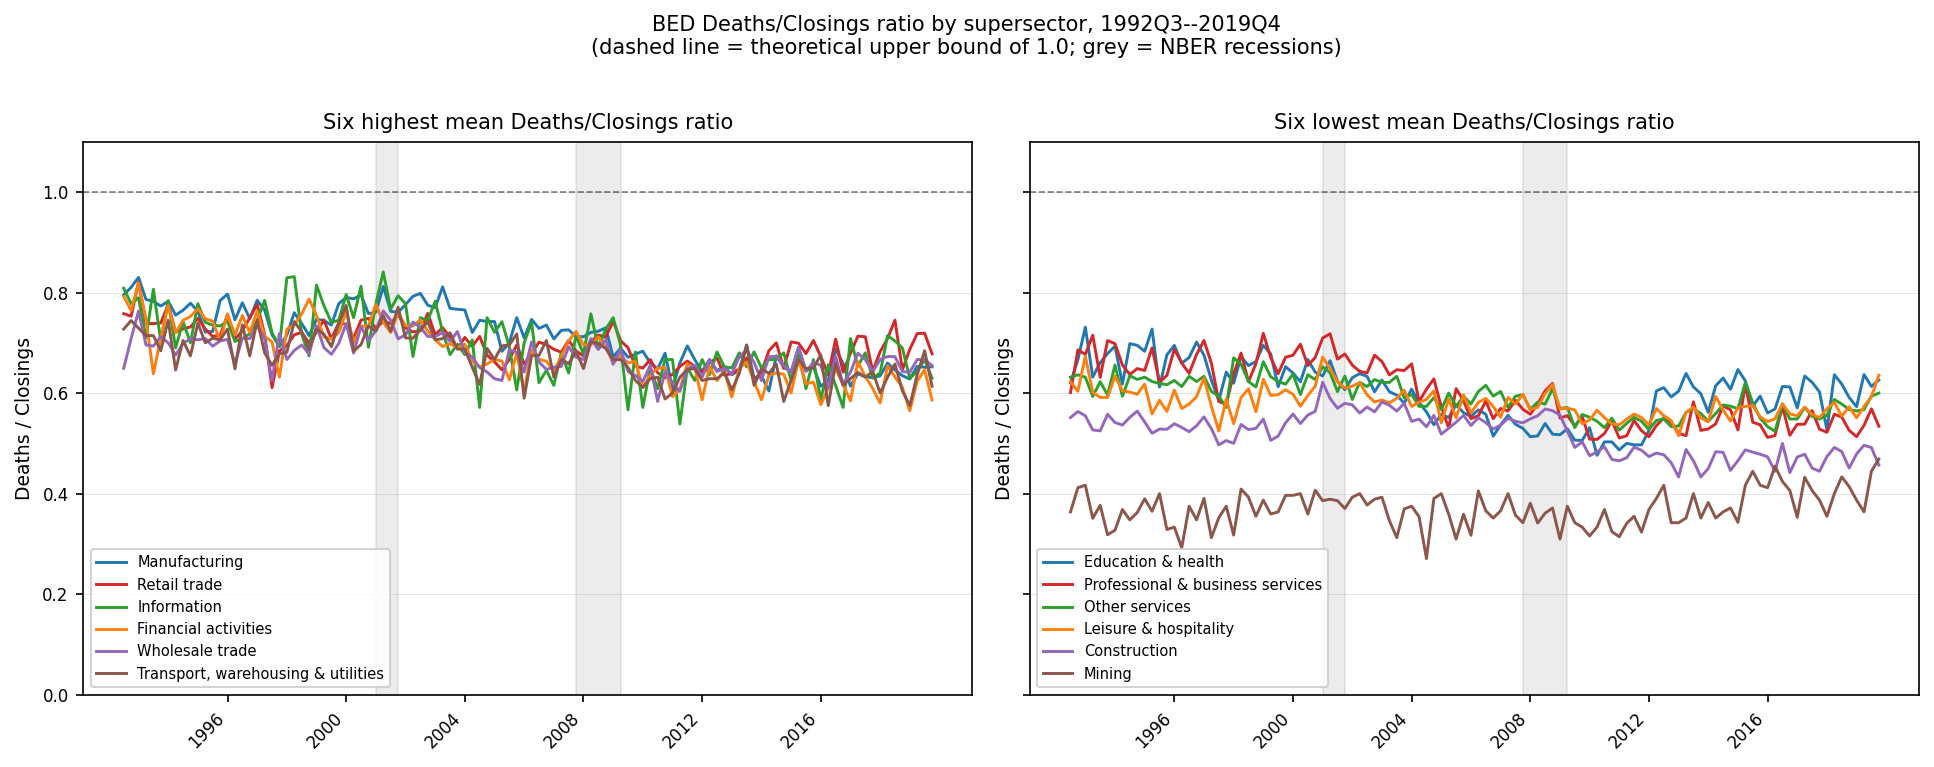
\includegraphics[width=\linewidth]{bed_deaths_by_supersector.png}
		\caption{BED Deaths/Closings ratio by supersector, 1992Q3--2019Q4.
			\emph{Left panel:} six supersectors with highest mean ratio.
			\emph{Right panel:} six supersectors with lowest mean ratio.
			Dashed horizontal line at 1.0 is the theoretical upper bound
			(Deaths $\subseteq$ Closings by construction).
			Grey shading denotes NBER recessions.}
		\label{fig:deaths_by_supersector}
	\end{figure}
	\subsection{Residual \texorpdfstring{$\delta$}{delta}--LD correlation}\label{app:delta_ld_corr}

	After v2 residualization the cross-state correlation between the $\delta$
	and layoffs-and-discharges instruments is
	$r(\tilde{B}^\delta, \tilde{B}^{\text{LD}}) = 0.334$, down from $0.54$
	on raw rates.  The residualization controls for aggregate productivity
	growth, lagged industry value-added, and lagged labor-market tightness,
	ruling out the most obvious industry-demand and aggregate-cycle
	explanations for the shared variation.  The leading interpretation is
	industry-specific financial conditions: when credit tightens in a sector,
	both product-line exit ($\uparrow \delta$) and layoffs at surviving
	establishments ($\uparrow \text{LD}$) rise simultaneously, generating
	positive covariance without a structural link between the two shocks.
	Consistent with this, the Granger-causality evidence shows that $\delta$
	predicts future LD at horizons $h = 4$--$12$ while LD predicts future
	$\delta$ only at $h = 0$--$4$; the long-horizon dependence runs from
	destruction to layoffs and not the reverse.  A natural further step
	would be to residualize on a measure of sector-level credit supply,
	such as SLOOS net C\&I tightening interacted with industry leverage
	exposure; we leave this for future work.

	\subsection{LD local projections}\label{app:ld_lp}

	The separate LD local projections are subsumed by the joint LP figure
	(Figure~\ref{fig:joint_lp_vacancy} below), which overlays the LD
	separate-specification IRF alongside the joint-LP coefficient for the
	same instrument.  In the separate specification the LD unemployment
	response rises monotonically to a peak of $+1.68$ pp at $h=20$,
	significant throughout, while the vacancy response is persistently
	negative (trough $-0.45$ pp at $h=20$).  Both patterns survive the
	severity placebo.  The monotonically rising unemployment IRF is
	anomalous given the estimated LD persistence
	$\hat\rho_{\text{LD}} \approx 0.3$: a transitory shock should produce
	a hump-shaped response, not a path that continues to rise five years
	out.  The most likely explanation is GFC contamination --- the 2008--09
	recession produced a severe and prolonged layoff episode whose
	industry-composition variation is not fully absorbed by the v2
	residualization --- rather than a structural property of the $s$ shock.
	We regard the LD IRFs as indicative rather than structural, and do not
	use them as estimation targets.

	\subsection{Joint local projection}\label{app:joint_lp}

	Figure~\ref{fig:joint_lp_vacancy} reports the joint versus separate
	local projections for the vacancy outcome.  Each panel overlays the
	joint-LP coefficient (red, solid) against the corresponding
	separate-LP coefficient (blue, solid), with 90\% confidence bands.

	\begin{figure}[H]
		\centering
		\includegraphics[width=\textwidth]{lp_joint_delta_ld_vacancy.png}
		\caption{Joint versus separate local projections: vacancy rate
			outcome.  \emph{Left panel:} $\delta$ instrument --- joint LP
			(red) vs.\ separate LP (blue).  \emph{Right panel:} LD
			instrument --- joint LP (red) vs.\ separate LP (blue).
			Shading denotes 90\% confidence intervals; standard errors
			clustered at the state level ($n=50$).  Instruments are
			v2-residualized; sample 2001Q1--2019Q4.}
		\label{fig:joint_lp_vacancy}
	\end{figure}

	Three findings emerge from the figure.  First, the $\delta$ vacancy IRF
	is qualitatively stable across specifications: the joint and separate
	coefficients share the same sign, timing, and shape throughout, and the
	confidence bands overlap at most horizons.  The trough in the joint
	specification ($-0.535$ pp at $h=5$) is somewhat shallower and earlier
	than in the separate specification ($-0.582$ pp at $h=18$), reflecting
	partial absorption of the shared variation with LD, but the persistent
	negative response to product-line destruction is not an artifact of LD
	exposure.

	Second, the $\delta$ unemployment IRF shrinks by roughly $0.6$--$0.8$
	pp in the joint specification relative to the separate LP, reflecting
	absorption of the variation that $\tilde{B}^\delta$ and
	$\tilde{B}^{\text{LD}}$ share.  The joint peak of $+1.15$ pp remains
	positive and significant, so the unemployment result is robust, if
	attenuated.

	Third, the LD vacancy coefficient collapses from its separate-LP value
	to approximately zero and is insignificant at all horizons once
	$\delta$ is controlled for (right panel).  This collapse should
	\emph{not} be read as evidence that $\delta$ subsumes a genuine LD
	effect on vacancies.  Rather, it reflects that
	$r(\tilde{B}^\delta,\tilde{B}^{\text{LD}})=0.334$ is large enough that
	the two instruments do not span orthogonal directions in the shock
	space: the variation in $\tilde{B}^{\text{LD}}$ orthogonal to
	$\tilde{B}^{\delta}$ is insufficient to separately identify the LD
	vacancy response.  The appropriate conclusion is that LD is not
	separately identified as a structural shock in this setting, not that
	separation shocks have zero causal effect on vacancies.

	We therefore treat the separate $\delta$ LP as the primary
	specification.  The joint LP establishes that the headline result ---
	a persistent vacancy decline in response to product-line destruction
	--- is robust to controlling for LD, and that the failure to separately
	identify LD is an instrument-space problem rather than a finding about
	vacancy dynamics.

	\subsection{QU placebo instrument}\label{app:qu_placebo}

	$\tilde{B}^{\text{QU}}$ is constructed from JOLTS quit rates using the
	same shares and residualization as the primary instruments.  Quits
	represent voluntary job-to-job transitions: the quitting worker moves
	directly to another employer, leaving the origin firm with an unfilled
	position but supplying the destination firm with a worker.  The net
	effect on aggregate unemployment and vacancies is therefore ambiguous
	and governed by matching frictions at the destination, not by the
	separation event at the origin.  This is conceptually distinct from the
	model's $s$ shock, which dissolves a match and triggers an unambiguous
	vacancy repost.  Furthermore, the quit rate is procyclical --- it rises
	when labor markets tighten --- so $\tilde{B}^{\text{QU}}$ partly
	reflects the same industry-level demand cycle that v2 residualization
	attempts to remove.

	Empirically, the QU instrument does not behave as a flat-zero placebo.
	Its unemployment and vacancy IRFs are nearly identical in magnitude to
	those of $\tilde{B}^\delta$, and the within-instrument correlation
	$\text{corr}(\hat\beta^u_h, \hat\beta^v_h) = -0.971$ across $h =
	0,\ldots,20$ --- the same mechanical proportionality observed for
	$\tilde{B}^\delta$ ($-0.948$).  This signature indicates that QU
	identifies industry-level demand contractions (which move $u$ and $v$
	symmetrically along the Beveridge curve) rather than a structurally
	distinct separation shock.  The contamination is likely structural:
	high-quit industries tend to be procyclical, so the industry component
	of the quit rate is correlated with demand conditions even after
	residualization on aggregate productivity and lagged VA.  The QU
	failure confirms that a well-identified $s$-type instrument remains an
	open challenge and motivates treating the LD results as indicative
	rather than structural.

	%%%%%%%%%%%%%%%%%%%%%%%%%%%%%%%%%%%%%%%%%%

	\subsection{Filter robustness for \texorpdfstring{$\delta$}{delta}-related moments}\label{app:filter_robustness}

	Table~\ref{tab:smm_moments} is computed with HP filter $\lambda=1{,}600$,
	departing from the $\lambda=10^5$ convention of \citep{shimer_2005, coles_2018} and other papers. Here we show that smoothening at $\lambda=10^5$ generates anomalous $\delta$ dynamic correlations with respect to other filters.

	Table~\ref{tab:dyn_corr_filter} reports dynamic cross-correlations
	$\text{cor}(\delta_t, x_{t+h})$ for $x \in \{u, v\}$ and
	$h \in \{-4, \ldots, +4\}$ under four conventions: HP with
	$\lambda=1{,}600$ and $\lambda=10^5$; the Hamilton (2018) regression
	filter (projection of $y_t$ on $y_{t-h},\ldots,y_{t-h-3}$ with $h=8$
	quarters); and first differences.  All series are log-transformed before
	filtering.

	First, $\text{cor}(\delta_t, u_{t+h})$ is
	positive at $h=0$ under every specification except $\lambda=100^5$
	(HP-100k: $+0.02$; HP-1600: $+0.39$; Hamilton: $+0.19$; FD: $+0.60$).
	Second, $\text{cor}(\delta_t, v_{t+h})$ is negative at $h=0$ and $h=+1$
	under HP-1600, Hamilton, and FD, while HP-100k delivers the opposite sign.
	HP-100k is flagged as an outlier at five of the nine horizons for the
	vacancy correlation.  

	\begin{table}[H]
	\centering
	\begin{threeparttable}
	\caption{Dynamic correlations $\text{cor}(\delta_t, x_{t+h})$ by detrending filter}
	\label{tab:dyn_corr_filter}
	\begin{tabular}{r rrrr @{\hspace{10pt}} rrrr}
	\toprule
	& \multicolumn{4}{c}{$x = $ Unemployment ($u$)} & \multicolumn{4}{c}{$x = $ Vacancies ($v$)} \\
	\cmidrule(lr){2-5}\cmidrule(lr){6-9}
	$h$ & HP-1600 & HP-100k & Hamilton & FD & HP-1600 & HP-100k & Hamilton & FD \\
	\midrule
	$-4$ & $-0.265$ & $-0.411$ & $-0.332$ & $-0.013$ & $ 0.296$ & $ 0.557$ & $ 0.448$ & $ 0.175$ \\
	$-3$ & $-0.343$ & $-0.435$ & $-0.334$ & $-0.115$ & $ 0.211$ & $ 0.490$ & $ 0.357$ & $ 0.068$ \\
	$-2$ & $-0.271$ & $-0.365$ & $-0.257$ & $-0.018$ & $ 0.089$ & $ 0.372$ & $ 0.229$ & $ 0.032$ \\
	$-1$ & $-0.197$ & $-0.309$ & $-0.176$ & $-0.414$ & $-0.029$ & $ 0.281$ & $ 0.085$ & $ 0.137$ \\
	$ 0$ & $+0.386$ & $+0.018$ & $+0.185$ & $+0.601$ & $-0.225$ & $+0.148$ & $-0.057$ & $-0.143$ \\
	$+1$ & $+0.216$ & $-0.048$ & $+0.172$ & $-0.129$ & $-0.312$ & $+0.065$ & $-0.143$ & $ 0.003$ \\
	$+2$ & $+0.198$ & $-0.031$ & $+0.158$ & $-0.026$ & $-0.384$ & $-0.005$ & $-0.205$ & $-0.197$ \\
	$+3$ & $+0.201$ & $-0.003$ & $+0.133$ & $-0.016$ & $-0.292$ & $+0.021$ & $-0.144$ & $-0.169$ \\
	$+4$ & $+0.215$ & $+0.031$ & $+0.122$ & $+0.127$ & $-0.058$ & $+0.133$ & $-0.028$ & $ 0.174$ \\
	\bottomrule
	\end{tabular}
	\begin{tablenotes}[flushleft]
	\footnotesize
	\item \textit{Note:} All series log-transformed before filtering.
	Sample: 1992Q3--2021Q4 ($N=118$); FD loses one observation.
	HP-1600: Hodrick-Prescott filter with $\lambda=1{,}600$.
	HP-100k: HP filter with $\lambda=10^5$.
	Hamilton: regression filter of \citet{hamilton_2018}, $h=8$ quarters, $p=4$ lags.
	FD: quarter-on-quarter first differences.
	Entries in \textbf{bold} indicate horizons where HP-100k has the opposite sign
	from all three other filters.
	\end{tablenotes}
	\end{threeparttable}
	\end{table}

	%%%%%%%%%%%%%%%%%%%%%%%%%%%%%%%%%%%%%%%%%%


	\section{Steady state}\label{app:steady_state}
	We summarize the steady state of the system below:
	\begin{align}
		%	p&=N^{1/(\varepsilon-1)}\\
		\nu^f&=\rho(N)f_e/\mu(N)\\
		w^{int}&=\rho(N)z/\mu(N)\\
		\frac{d^f}{\nu^f}&=\frac{r+\delta_e}{1-\delta_e}\\
		\kappa+\frac{K}{q(\theta)}&=\frac{1-\delta_e}{r+\tau}(w^{int}-w-K-s\mathcal{R})\\
		%\frac{\gamma P}{q(\theta)}&=\frac{z/\mu-w}{\rho+s}\\
		%\gamma N^{1/(1-\varepsilon)}\left[\frac{\rho+s}{q(\theta)}+\phi \theta\right]&=(1-\phi)\left(pz/\mu-b-K\right)\\
		w &= \phi \left[ w^{int}-K+\theta(K+q(\theta)\kappa)-s\mathcal{R}\right]+(1-\phi)b\\
		\mathcal{R}&=\frac{1-\delta_e}{1+r}\left(Q-Q^{rep}\right),\quad
		Q^{rep}=Q\Lambda_r-\psi_cQ(\Lambda_r-1+p_0),\quad
		\Lambda_r=F(Q/\alpha)\\
		Q&=e^{1/\xi}x_m \\
		1-\delta_e&=(1-\delta)F(\chi^c),\quad \tau=1-(1-\delta_e)(1-s)\\
		K&=\frac{r+\delta_e}{1+r}Q\\
		u&=\frac{\tau}{\tau+(1-\delta_e)f(\theta)}\label{eq:u_ss}\\
		e&=\delta_e(v+1-u)+(1-\delta_e)(1-\Lambda_r)s(1-u)\label{eq:e_ss}\\
		N^e&=\delta_e N/(1-\delta_e)\\
		L^c&=\frac{r+\delta_e}{r+\delta_e+\delta_e \pi_s \mu}L,\quad L^e=\frac{\delta_e \pi_s \mu}{r+\delta_e+\delta_e\pi_s \mu}L\label{eq:labor_ss}\\
		\chi^c&=\frac{\rho f_e}{\mu}\left(\frac{r+\delta_e}{1-\delta_e}\frac{\mu-1}{\mu \pi_s}+1\right)\\
		\pi_s&=\frac{\mu-1}{\mu}\frac{(1-\psi_c\varpi)(r+\delta_e)}{r+\delta_e+\psi_c\varpi(1-\delta_e)},\quad \varpi=1-\frac{(1-p_0)(1-\delta)}{1-\delta_e}\\
		Y^{Gross}&=Y^C+\nu^f N^e=w^{int}L+Nd^f\\
		Y&=C+\nu^fN^e\\
		X&=e\frac{\xi}{\xi+1}Q+\kappa qv\\
		X^c&=N\psi_c\varpi\chi^c\\
		X^r&=(1-\delta_e)s(1-u)\,\psi_cQ(\Lambda_r-1+p_0)\\
		Y^c&=\rho zL^c=C+X+X^c+X^r\\
	\end{align}
	Most of these equations are self-evident from the equilibrium system. For instance, evaluating \eqref{eq:u_lom} yields \eqref{eq:u_ss}. The forms of $Q^{rep}$ and $X^r$ use the interior closed form of the reactivation-cost integral derived below~\eqref{eq:agg_repost_costs}. To find $e$, start with the steady-state vacancy law of motion:
	\begin{align}
		[1-(1-\delta_e)(1-q)]v=(1-\delta_e)\Lambda_r s(1-u)+e
	\end{align}
	Expanding the left-hand side as $\delta_e v+(1-\delta_e)qv$ and rewriting $(1-\delta_e)qv=\tau(1-u)$, we have
	\begin{align}
		\delta_e v+\tau(1-u)=(1-\delta_e)\Lambda_r s(1-u)+e\\
		\delta_e v + [\tau-(1-\delta_e)\Lambda_r s](1-u)=e
	\end{align}
	and since $\tau-(1-\delta_e)\Lambda_r s=\delta_e+(1-\delta_e)(1-\Lambda_r)s$, we obtain~\eqref{eq:e_ss}. New entrants replace two kinds of lost positions: those destroyed with exiting product lines, $\delta_e(v+1-u)$, and those retired at surviving product lines because they were not reactivated. With costless reposting ($\Lambda_r=1$) only the first remains, $e=\delta_e(v+1-u)$, and the contribution of entrants to the vacancy pool is governed by the total exit rate $\delta_e$ alone.
	
	At $p_0=0$, where $X^c=0$, labor in entry follows directly from the resource constraint curve:
	\begin{align}
		L^e&=\frac{\delta_e}{1-\delta_e}Nf_e/z\\
		&=\frac{\delta_e}{1-\delta_e}\left[\frac{(\mu-1)zL(1-\delta_e)}{f_e(\delta_e \mu+r)}\right]f_e/z\\
		&=\frac{\delta_e(\mu-1)}{\delta_e \mu+r}L
	\end{align}
	The steady-state job creation and wage equations can be arranged as
	\begin{align}\label{eq:jcc_wage_ss}
		\kappa+\frac{K}{q}=\frac{1-\delta_e}{r+\tau}\left[(1-\phi)(w^{int}-K-b)-\phi \theta q\!\left(\kappa+\frac{K}{q}\right)-(1-\phi)s\mathcal{R}\right]
	\end{align}
	Equation \eqref{eq:jcc_wage_ss} equates the average recruiting cost to the present-discounted value of the match, adjusted for the wage bargain. The right-hand side incorporates a fraction $1-\phi$ of the flow surplus $(w^{int}-K-b)$, an adjustment for the outside option of the worker, and the recruiter's share $1-\phi$ of the expected reposting shortfall, which vanishes with costless reposting. Whereas in the standard DMP model, the analogous expression would characterize tightness, here $K$ and $w^{int}$ are additional endogenous variables. Moreover, the average recruiting cost has the compound form $\kappa+K/q$, and discounting is adjusted by the overall firm survival rate $1-\delta_e$.
	
	\section{Derivations}
	\subsection{Preference specifications}\label{app:preferences}
	Table~\ref{tab:preference_specifications} reports the two statistics that characterize
	symmetric homothetic preferences in the model, $\mu(N)$ and $\rho(N)$, with the implied
	benefit of variety $\zeta(N)$, under three specifications. DS-CES is the quantitative
	baseline. Generalized CES \citep{benassy_1996} has consumption basket
	$N^{\zeta-1/(\varepsilon-1)}\bigl(\int c_j^{(\varepsilon-1)/\varepsilon}dj\bigr)^{\varepsilon/(\varepsilon-1)}$,
	so $\zeta$ and $\varepsilon$ are separate parameters. Under the translog expenditure function
	of \citet{feenstra_2003}, the price elasticity of demand is $\varepsilon(N)=1+\eta N$, so
	goods become more substitutable as variety increases, and $\tilde{N}$ is the mass of all
	potential goods.

	\begin{table}[H]
		\centering
		\begin{tabular}{l|ccc}
			\toprule
			& DS-CES & General CES & Translog \\
			\midrule
			Consumption index
			& $\left(\int c_j^{(\varepsilon-1)/\varepsilon}dj
			\right)^{\varepsilon/(\varepsilon-1)}$
			& $N^{\zeta-1/(\varepsilon-1)}\left(\int
			c_j^{(\varepsilon-1)/\varepsilon}dj
			\right)^{\varepsilon/(\varepsilon-1)}$
			& $-$ \\
			Price index
			& $\left(\int p_j^{1-\varepsilon}dj
			\right)^{1/(1-\varepsilon)}$
			& $N^{-\zeta+1/(\varepsilon-1)}\left(\int
			p_j^{1-\varepsilon}dj\right)^{1/(1-\varepsilon)}$
			& $-$ \\
			Markup $\mu(N)$
			& $\frac{\varepsilon}{\varepsilon-1}$
			& $\frac{\varepsilon}{\varepsilon-1}$
			& $1+\frac{1}{\eta N}$ \\
			Relative price $\rho(N)$
			& $N^{\frac{1}{\varepsilon-1}}$
			& $N^{\zeta}$
			& $\exp\left\{-\frac{1}{2}
			\frac{\tilde{N}-N}{\eta \tilde{N}N}\right\}$ \\
			Benefit of variety $\zeta(N)$
			& $\mu-1$
			& $\zeta$
			& $\frac{1}{2\eta N}=\frac{\mu(N)-1}{2}$ \\
			\bottomrule
		\end{tabular}
		\caption{Preference specifications: indices, markup, relative
			price, and benefit of variety.}
		\label{tab:preference_specifications}
	\end{table}

	\subsection{Relationship between profit share and power law shape parameter $\psi$}
Write $\varpi\equiv1-(1-p_0)(1-\delta)/(1-\delta_e)$ for the steady-state share of
surviving lines that drew a positive continuation cost, $p_0(\chi^c/\chi_m)^\psi/\Lambda$
with $\Lambda=(1-\delta_e)/(1-\delta)$, so that $X^c=N\psi_c\varpi\chi^c$ by
\eqref{eq:agg_fixed_costs}. The cutoff satisfies $\chi^c=Y^c(\mu-1)/(\mu N)+\rho f_e/\mu$,
so $X^c=\psi_c\varpi\bigl(Y^c(\mu-1)/\mu+N\rho f_e/\mu\bigr)$. Dividing by $Y^c=\rho zL^c$,
\begin{align*}
	\frac{X^c}{Y^c}=\frac{\psi_c\varpi}{\mu}\left(\mu-1+\frac{f_eN}{zL^c}\right).
\end{align*}
The steady-state business formation Euler equation gives $d^f/\nu^f=(r+\delta_e)/(1-\delta_e)$,
and with $Nd^f=\pi_sY^c$ this is $f_eN/(zL^c)=\mu\pi_s(1-\delta_e)/(r+\delta_e)$. Since
$\pi_s=(\mu-1)/\mu-X^c/Y^c$,
\begin{align*}
	\pi_s=\frac{\mu-1}{\mu}(1-\psi_c\varpi)-\frac{\psi_c\varpi(1-\delta_e)\pi_s}{r+\delta_e},
\end{align*}
and solving for $\pi_s$,
\begin{align}\label{eq:profit_share_ss}
	\pi_s=\frac{\mu-1}{\mu}\frac{(1-\psi_c\varpi)(r+\delta_e)}{r+\delta_e+\psi_c\varpi(1-\delta_e)}.
\end{align}
Holding $\delta_e$ fixed, $\pi_s$ falls with $\psi_c\varpi$. For $\psi_c\varpi=0$,
$\pi_s=(\mu-1)/\mu=1/\varepsilon$, as in \citet{bilbiie_2012}. The cutoff in terms of the
profit share is
\begin{align*}
	\chi^c&=\frac{\rho}{\mu}\left(\frac{zL^c(\mu-1)}{N}+f_e\right)
	=\frac{\rho f_e}{\mu}\left(\frac{r+\delta_e}{1-\delta_e}\frac{\mu-1}{\mu \pi_s}+1\right)
	=\frac{\rho f_e}{\mu}\,\frac{1+r}{(1-\delta_e)(1-\psi_c\varpi)},
\end{align*}
which is \eqref{eq:exit_threshold_curve}.

\subsection{Resource constraint curve}
Write $c\equiv\psi_c\varpi$. Rearranging~\eqref{eq:labor_N} as
$N=zL(1-\delta_e)/\bigl[f_e\bigl((r+\delta_e)/(\mu\pi_s)+\delta_e\bigr)\bigr]$ and substituting
\eqref{eq:profit_share_ss},
\begin{align*}
	N=\frac{(\mu-1)(1-c)\,zL(1-\delta_e)}{f_e\bigl[\delta_e\mu+r+c(1-\mu\delta_e)\bigr]},
\end{align*}
which reduces to \eqref{eq:curve_res_cons} at $c=0$. Labor in entry and in the consumption
sector are then
\begin{align*}
	L^e=\frac{\delta_e}{1-\delta_e}\frac{Nf_e}{z}
	=\frac{\delta_e(\mu-1)(1-c)}{\delta_e\mu+r+c(1-\mu\delta_e)}\,L,
	\qquad
	L^c=\frac{r+\delta_e+c(1-\delta_e)}{\delta_e\mu+r+c(1-\mu\delta_e)}\,L,
\end{align*}
consistent with \eqref{eq:labor_ss}, and the continuation-cost share of gross consumption
output is
\begin{align*}
	\frac{X^c}{Y^c}=\frac{c\,(\mu-1)(1+r)}{\mu\bigl[r+\delta_e+c(1-\delta_e)\bigr]}.
\end{align*}
%\eqref{eq:curve_res_cons}.
\subsection{Labor share of GDP}
	The aggregate resource constraint can be rearranged to pin down the income of recruiters:
	\begin{align}
		w^{int}L=\frac{Y^c}{\mu}+\nu^f N^e
	\end{align}
	Thus, the income share of recruiters relative to gross output is
	\begin{align}
		\frac{w^{int}L}{Y^{Gross}}&=\pfrac{r+\delta_e}{r+\delta_e+\delta_e \pi_s}\frac{1}{\mu}+\frac{\delta_e\pi_s}{r+\delta_e+\pi_s}\\
		&=\frac{r+\delta_e+\delta_e \mu \pi_s}{\mu(r+\delta_e+\delta_e\pi_s)}
	\end{align}
	The labor share of GDP is
	\begin{align}
		\frac{wL}{Y} = (1+\frac{X+X^c+X^r}{Y})\frac{w}{w^{int}}\frac{r+\delta_e+\delta_e \mu \pi_s}{\mu(r+\delta_e+\delta_e\pi_s)}
	\end{align}
	The steady-state labor share is composed of three factors. The first factor just reflects the wedge between gross output and GDP, which depends on the recruiting, fixed, and reactivation cost shares. The second and third comprise a search wedge $w/w^{int}$ and a market power wedge $w^{int}L/Y^{Gross}$. Through the latter, the labor share depends positively on $\delta_e$ and $\rho$, and negatively on $\pi_s$. Intuitively, a higher product destruction rate requires more labor resources, and thus income accruing to labor. A higher price markup raises profits and thus lowers the labor share. Indeed, in standard DSGE models with monopolistic competition, the labor share just the inverse of the price markup. Here that arises as a limiting case in which search frictions vanish ($w\to w^{int}$) and $\delta \to 0$. The latter entails eliminating the entry sector, which affects the labor share since only retailers charge markups. Note that the search wedge, in turn, depends on $\phi$ and $b$. Moreover, variety effects affect the search wedge through $w^{int}$ but otherwise do not affect the steady-state shares.
	
	The special case studied by \citet{bilbiie_2012} arises if we shut down labor market frictions and fixed costs in production. In this limit $\delta_e=\delta$ (no endogenous exit), $w^{int}=w$, $X=X^c=0$, and $\pi_s=1/\varepsilon$, giving
	\begin{align}
		\frac{wL}{Y}=\frac{(r+\delta)(\varepsilon-1)+\delta}{\varepsilon(r+\delta)+\delta}=\frac{C}{Y}\frac{1}{\mu}+\frac{\nu^f N^e}{C}
	\end{align}
	which equals the consumption share divided by the markup plus the entry share.
	
	\subsection{Wage determination}\label{app:wage}
	We derive the Nash wage~\eqref{eq:wage_eq}. Start from the value of the large household:
	\begin{align}
		W_t&=\max_{c_t,a_{t+1}} \frac{c_t^{1-\sigma}}{1-\sigma}+\beta \mathbb{E}_t W_{t+1} \quad \text{s.t.}\\
		&c_t+\nu_ta_{t+1}=w_tL_t+b(1-L_t)+(\nu_t+d_t)a_t+D_t^{int} -T_t
	\end{align}
	which is~\eqref{eq:bc_HH} with $L_t=1-u_t$. Given the continuum of members in a household, the surplus of moving an unemployed member into employment is $\der{W_t}{L_t}$. Nash bargaining solves
	\begin{align}\label{eq:Nash_product}
		w_t=\arg \max \left[\der{W_t(w_t)}{L_t}\right]^{\phi}\left[J_t(w_t)-Q_t\right]^{1-\phi}
	\end{align}
	For convenience, define the match surpluses $S_t^H\equiv\der{W_t}{L_t}$ and $S_t^J\equiv J_t-Q_t$.

	By the envelope theorem,
	\begin{align}\label{eq:HH_envelope}
		S_t^H=c_t^{-\sigma}\der{c_t}{L_t}+\beta \mathbb{E}_t\left[S_{t+1}^H\der{L_{t+1}}{L_t}\right]
	\end{align}
	From the budget constraint, $\der{c_t}{L_t}=w_t-b$. Employment evolves as
	\begin{align}\label{eq:L_lom}
		L_{t+1}=(1-\delta_{e,t+1})\bigl[(1-s_t)L_t+f(\theta_t)(1-L_t)\bigr]
	\end{align}
	A match survives into $t+1$ only if its product line survives both exogenous destruction and the continuation-cost draw, with probability $1-\delta_{e,t+1}=(1-\delta_t)F(\chi_{t+1}^c)$ from~\eqref{eq:delta_e_lom}. Matches formed at $t$ face product-line exit but not match separation before they first produce. This is the timing of the recruiter values~\eqref{eq:value_recruiter_unmatched} and~\eqref{eq:value_recruiter_matched} and of the vacancy law of motion~\eqref{eq:v_lom}. Partial reposting does not enter~\eqref{eq:L_lom}: it governs whether a vacated position returns as a vacancy, not whether the worker separates. Hence
	\begin{align}
		\der{L_{t+1}}{L_t}=(1-\delta_t)F(\chi_{t+1}^c)\left(1-s_t-f(\theta_t)\right)
	\end{align}
	and, since $s_t$, $\delta_t$, and $\theta_t$ are known at $t$,
	\begin{align}\label{eq:SH_bellman}
		S_t^H=c_t^{-\sigma}(w_t-b)+\left(1-s_t-f(\theta_t)\right)\beta(1-\delta_t)\mathbb{E}_t\left[F(\chi_{t+1}^c)S_{t+1}^H\right]
	\end{align}

	The first-order condition of~\eqref{eq:Nash_product} is
	\begin{align}
		\phi \frac{\der{S_t^H}{w_t}}{S_t^H}+(1-\phi)\frac{\der{S_t^J}{w_t}}{S_t^J}=0
	\end{align}
	The next-period wage is re-bargained under next-period conditions, so the continuation term in~\eqref{eq:SH_bellman} does not move with $w_t$ and $\der{S_t^H}{w_t}=c_t^{-\sigma}$. From~\eqref{eq:value_recruiter_surplus}, the recruiter surplus is
	\begin{align}\label{eq:SJ_app}
		S_t^J=w_t^{int}-w_t-K_t +(1-s_t)\left(\kappa+\frac{K_t}{q(\theta_t)}\right)-s_t\mathcal{R}_t
	\end{align}
	where $\mathcal{R}_t$ is the expected discounted reposting shortfall~\eqref{eq:repost_shortfall}. It depends only on period-$t+1$ objects, so $\der{S_t^J}{w_t}=-1$, and the first-order condition gives the sharing rule
	\begin{align}\label{eq:sharing_rule}
		S_t^H=\frac{\phi}{1-\phi}c_t^{-\sigma}S_t^J
	\end{align}

	Forwarding~\eqref{eq:sharing_rule} one period and using $m_{t+1}=\beta(c_{t+1}/c_t)^{-\sigma}$,
	\begin{align}
		\beta(1-\delta_t)\mathbb{E}_t\left[F(\chi_{t+1}^c)S_{t+1}^H\right]
		=\frac{\phi}{1-\phi}c_t^{-\sigma}\,\mathbb{E}_tm_{t+1}(1-\delta_t)F(\chi_{t+1}^c)S_{t+1}^J
		=\frac{\phi}{1-\phi}c_t^{-\sigma}\left(\kappa+\frac{K_t}{q(\theta_t)}\right)
	\end{align}
	where the second equality is the job creation condition~\eqref{eq:jcc}. Substituting into~\eqref{eq:SH_bellman},
	\begin{align}
		S_t^H=c_t^{-\sigma}\left[w_t-b+\left(1-s_t-f(\theta_t)\right)\frac{\phi}{1-\phi}\left(\kappa+\frac{K_t}{q(\theta_t)}\right)\right]
	\end{align}
	Equating~\eqref{eq:SJ_app} with $S_t^J$ from the sharing rule~\eqref{eq:sharing_rule} gives
	\begin{align}
		w_t^{int}-w_t-K_t+(1-s_t)\left(\kappa+\frac{K_t}{q(\theta_t)}\right)-s_t\mathcal{R}_t=\frac{1-\phi}{\phi}\left(w_t-b\right)+\left(1-s_t-f(\theta_t)\right)\left(\kappa+\frac{K_t}{q(\theta_t)}\right)
	\end{align}
	Solving for the wage,
	\begin{align}
		w_t=\phi\left(w_t^{int}-K_t+f(\theta_t)\left(\kappa+\frac{K_t}{q(\theta_t)}\right)-s_t\mathcal{R}_t\right)+(1-\phi)b
	\end{align}
	The household surplus carries no reposting term: a separated worker becomes unemployed whether or not the recruiter reactivates the vacated position. The shortfall therefore enters bargaining only through the recruiter's surplus, and the worker bears share $\phi$ of it through a lower wage. The term acts like a firing cost, except that separation is exogenous. Costless reposting ($\alpha\to0$ or $p_0=0$) gives $\mathcal{R}_t=0$ and recovers the wage without reposting.

	Substituting the wage back into~\eqref{eq:SJ_app} gives the wage-substituted surplus
	\begin{align}
		S_t^J=(1-\phi)\left(w_t^{int}-K_t-b\right)-\phi\theta_t\left(K_t+q(\theta_t)\kappa\right)+(1-s_t)\left(\kappa+\frac{K_t}{q(\theta_t)}\right)-(1-\phi)s_t\mathcal{R}_t
	\end{align}
	The recruiter bears only its bargaining share $1-\phi$ of the reposting shortfall.
\subsection{Log-linearized propagation equations}
\label{app:loglin}

This appendix collects log-linearized versions of the equations that govern
impulse-response dynamics.  Let a hat denote the log-deviation from the
deterministic steady state: $\hat{x}_t \equiv \ln(x_t/\bar{x})$, so
$x_t \approx \bar{x}(1+\hat{x}_t)$.  For rates that are small at steady
state ($\delta_e, s, \tau, u, v \ll 1$), we use the level deviation
$\tilde{x}_t \equiv x_t - \bar{x}$ directly and note $\tilde{x}_t \approx
\bar{x}\hat{x}_t$.   We present equations in the order in which they feed into one
another: the exit margin first, then the variety stock, the labor market, and
finally the vacancy-value chain. The equations describe the model with
costless reposting ($\alpha\to0$), which is the model solved for the
comparisons in Section~\ref{sec:mechanism_irfs}. Partial reposting adds
$\bar\Lambda_r$ to the reposting inflow in the vacancy law of motion and the
shortfall $\mathcal{R}_t$ to the recruiter surplus.

\paragraph{1.\ Endogenous exit rate}
The survival probability is $\Lambda_t \equiv F(\chi_t^c) = (1-p_0)+p_0(\chi_t^c/\chi_m)^\psi$,
and the total exit rate is~\eqref{eq:delta_e_lom}:
\begin{align}
    \delta_{e,t} = 1-(1-\delta_{t-1})\,\Lambda_t,
\end{align}
which in steady state is $\bar\delta_e = 1-(1-\bar\delta)\bar\Lambda$.
Define
    $\varsigma \;\equiv\; \left(\frac{\bar\chi^c}{\chi_m}\right)^\psi$, so that $\bar\Lambda = (1-p_0)+p_0\varsigma$ and $1-\bar\Lambda = p_0(1-\varsigma)$.

Totally differentiating around steady state:
\begin{align}
    d\delta_{e,t}
    \;=\; \bar\Lambda\,d\delta_{t-1}
    \;-\; (1-\bar\delta)\,\frac{d\Lambda_t}{d\chi_t^c}\,d\chi_t^c.
\end{align}
The derivative of $\Lambda$ with respect to $\chi^c$ at steady state is
\begin{align}
    \frac{d\Lambda}{d\chi^c}\bigg|_{\bar\chi^c}
    \;=\; \frac{p_0\,\psi\,\varsigma}{\bar\chi^c}.
\end{align}
Dividing through by $\bar\delta_e$ and writing $d\delta_{t-1}/\bar\delta = \hat\delta_{t-1}$,
$d\chi^c/\bar\chi^c = \hat\chi_{c,t}$:
\begin{align}\label{eq:delta_e_ll}
    \hat{\delta}_{e,t}
    \;=\; \frac{\bar\Lambda}{\bar\delta_e}\,\bar\delta\,\hat\delta_{t-1}
    \;-\; \frac{(1-\bar\delta)\,p_0\psi\varsigma}{\bar\delta_e}\,\hat\chi_{c,t}.
\end{align}
Define the \emph{exit elasticity} $\varepsilon_x$ as the elasticity of the endogenous exit
probability $(1-\Lambda_t)$ with respect to $\chi^c$:
\begin{align}\label{eq:dest_elast_def}
    \varepsilon_x \;\equiv\;
    \frac{d(1-\Lambda)}{d\chi^c}\,\frac{\bar\chi^c}{1-\bar\Lambda}
    \;=\; \frac{p_0\psi\varsigma}{p_0(1-\varsigma)}
    \;=\; \frac{\psi\varsigma}{1-\varsigma}.
\end{align}
Since $p_0(1-\varsigma) = 1-\bar\Lambda$, equation~\eqref{eq:delta_e_ll} becomes
\begin{align}\label{eq:delta_e_ll_compact}
    \hat{\delta}_{e,t}
    \;=\; \frac{\bar\Lambda}{\bar\delta_e}\,\bar\delta\,\hat\delta_{t-1}
    \;-\; \frac{(1-\bar\delta)(1-\bar\Lambda)}{\bar\delta_e}\,\varepsilon_x\,\hat\chi_{c,t}.
\end{align}
Both coefficients are positive and $\hat\chi^c$ enters with a negative sign:
a higher continuation threshold raises survival and lowers $\delta_{e,t}$.
At the baseline calibration $\varepsilon_x=5$, meaning a 1\,\% rise in $\chi^c$
raises the endogenous exit probability $(1-\Lambda_t)$ by 5\,\%.

\paragraph{2.\ Continuation threshold}
From the cutoff condition~\eqref{eq:cutoff_free_entry} with $\mu$ constant
and $\rho(N_t) = N_t^{1/(\varepsilon-1)}$:
\begin{align}\label{eq:xc_ll}
    \hat\chi_{c,t}
    = \underbrace{\alpha_\pi\Bigl(\hat{Y}_{c,t} - \hat{N}_t\Bigr)}_{\text{profit component}}
    \;+\; \underbrace{(1-\alpha_\pi)\,\frac{1}{\varepsilon-1}\hat{N}_t}_{\text{continuation-value component}},
\end{align}
where $\alpha_\pi \equiv \bar{R}^f/\bar\chi^c \in(0,1)$ is the steady-state
share of per-firm gross profit in the threshold.  The profit component
(elasticity $\alpha_\pi\cdot\frac{\varepsilon-2}{\varepsilon-1} < 0$ in $N$
for $\varepsilon>2$) rises when $N$ falls, reflecting the market-share gain
to surviving firms under DS-CES demand.  The continuation-value component
(elasticity $(1-\alpha_\pi)/(\varepsilon-1) > 0$ in $N$) falls when $N$
falls, because the option value $\nu_f = \rho f_e/\mu$ shrinks with $\rho$.
The two forces partially offset: whether $\hat\chi^c$ rises or falls in
response to $\hat{N}<0$ depends on calibrated $\alpha_\pi$ and $\varepsilon$.

\paragraph{3.\ Firm stock (variety LOM)}
Log-linearizing the firm law of motion $N_{t+1}=(1-\delta_{e,t})(N_t+N_t^e)$
around steady state (using $\bar{N}^e/\bar{N}=\bar\delta_e/(1-\bar\delta_e)$):
\begin{align}\label{eq:N_lom_ll2}
    \hat{N}_{t+1}
    = (1-\bar\delta_e)\,\hat{N}_t
    \;+\; \bar\delta_e\,\hat{N}_t^e
    \;-\; \hat{\delta}_{e,t},
\end{align}
where the last term uses $(1+\bar{N}^e/\bar{N})\approx1/(1-\bar\delta_e)$ so
the exit rate enters with unit coefficient in absolute log-deviation terms.
The three forces are: (i)~\emph{mean reversion} at rate $\bar\delta_e$ — the
survival coefficient $(1-\bar\delta_e)$ governs how long any $N$ deviation
persists; (ii)~\emph{entry amplification} — the loading $\bar\delta_e$ on
$\hat{N}^e$ is larger when steady-state churning is higher, so the same
entry impulse produces a larger $N$ response; (iii)~the \emph{exit margin}
$\hat\delta_{e,t}$ from~\eqref{eq:delta_e_ll}, which feeds back through $\chi^c$.
Combining (i) and (ii): models with higher $\bar\delta_e$ show larger
amplitude but faster convergence; models with lower $\bar\delta_e$ show
smaller but more persistent deviations.  This is the common mechanism
underlying Comparisons~A and~B.

\paragraph{4.\ Interior wage (recruiter compensation)}
From $w_t^{int} = \rho(N_t) z_t/\mu$~\eqref{eq:recruiter_compensation} with
$\rho(N_t) = N_t^{1/(\varepsilon-1)}$:
\begin{align}\label{eq:wint_ll}
    \hat{w}_t^{int} = \frac{1}{\varepsilon-1}\,\hat{N}_t + \hat{z}_t.
\end{align}
This is the \emph{variety channel}: a contraction of the firm stock $N$
reduces the relative price $\rho$ (fewer varieties lower the CES price
index), compressing the marginal revenue product of labor $w^{int}$ even
holding productivity constant.  The elasticity $1/(\varepsilon-1)\approx0.30$
at $\varepsilon=4.3$ is moderate but cumulates over the slow $N$ recovery.

\paragraph{5.\ Aggregate separation rate}
From $\tau_t = \delta_{e,t}+s_{t-1}(1-\delta_{e,t})$~\eqref{eq:tau_lom},
log-linearizing:
\begin{align}\label{eq:tau_ll}
    \hat\tau_t
    = (1-\bar{s})\frac{\bar\delta_e}{\bar\tau}\,\hat\delta_{e,t}
    + \frac{\bar{s}(1-\bar\delta_e)}{\bar\tau}\,\hat{s}_{t-1},
\end{align}
where the coefficients sum to $1-\bar{s}\bar\delta_e/\bar\tau$, which is close to one, since
$\bar\tau=\bar\delta_e+\bar{s}(1-\bar\delta_e)$.  With the calibrated ratio
$\bar\delta_e/\bar\tau\approx0.21$, firm exit contributes about one-fifth of
aggregate separation variance; match-level separations account for the rest.

\paragraph{6.\ Unemployment LOM}
From~\eqref{eq:u_lom}, log-linearizing around $(\bar{u},\bar\tau,\bar{f})$:
\begin{align}\label{eq:u_ll}
    \tilde{u}_{t}
    = \bigl(1-(1-\bar\delta_e)\bar{f}-\bar\tau\bigr)\,\tilde{u}_{t-1}
    + (1-\bar{u})\,\tilde\tau_t
    + \bar{u}\bar{f}\,\tilde\delta_{e,t}
    - \bar{u}(1-\bar\delta_e)\,\tilde{f}_{t-1},
\end{align}
where $\tilde{x}_t = x_t-\bar{x}$ denotes the level deviation and
$\tilde{f}_t = f(\theta_t)-\bar{f}$.  The term in
$\tilde\delta_{e,t}$ is the exit exposure of matches formed in
$t-1$, which have not yet produced. The autoregressive coefficient
$(1-(1-\bar\delta_e)\bar{f}-\bar\tau)$ governs unemployment persistence: with monthly
$\bar{f}\approx0.40$ and $\bar\tau\approx0.031$, it equals approximately
$0.57$, giving an unemployment half-life of around two months in the absence
of sustained $\tau$ or $\theta$ shocks.  A $\delta$ shock is persistent
precisely because it generates a sustained $\tilde\tau_t>0$ through
$\tilde\delta_{e,t}>0$ and, via the variety channel~\eqref{eq:wint_ll}, a
sustained $\tilde{f}_{t-1}<0$ through the depressed JCC.

\paragraph{7.\ Vacancy LOM}
From~\eqref{eq:v_lom}, splitting into predetermined and new-entrant
components:
\begin{align}\label{eq:v_ll}
    \tilde{v}_t
    = (1-\bar\delta_e)\Bigl[(1-\bar{q})\,\tilde{v}_{t-1}
      + \bar{s}(1-\bar{u})\,\hat{s}_{t-1}\Bigr]
    - \bar{v}^{\mathrm{pre}}\,\tilde\delta_{e,t}
    + \tilde{e}_t,
\end{align}
where $\bar{v}^{\mathrm{pre}} = \bar{v}-\bar{e}$ is the steady-state predetermined vacancy stock.
As in~\eqref{eq:u_ll}, $\delta_e$ enters in level deviations and $s$ in log
deviations, matching their coefficients: $\partial[(1-\delta_e)x]/\partial\delta_e
=-x$, while the reposting term carries $\bar{s}$ already.
The three terms capture: (i)~\emph{survival of existing vacancies}, which
depends on $(1-\bar\delta_e)$ and amplifies the persistence asymmetry
between high- and low-$\delta_e$ specifications; (ii)~\emph{destruction
impulse} $\hat\delta_{e,t}$, which directly destroys the predetermined stock;
and (iii)~\emph{new entrant vacancies} $\tilde{e}_t$, which respond
contemporaneously to the vacancy-value signal $Q_t$.
The sunk-cost predetermination means that $\tilde{v}_t^{\mathrm{pre}}$
cannot adjust within the period, so the vacancy response to a $\delta$ shock
is asymmetrically slow relative to unemployment, consistent with the
empirical Beveridge curve dynamics in Section~\ref{sec:empirical_results}.

\paragraph{8.\ Vacancy value and new postings}
From~\eqref{eq:Kdef}, log-linearizing under a one-shock approximation
($\mathbb{E}_t\hat{Q}_{t+1}=\rho_x\hat{Q}_t$, exact by undetermined
coefficients for shock $x\in\{z,\delta\}$ with persistence $\rho_x$):
\begin{align}\label{eq:Q_ll2}
    \hat{Q}_t
    = \underbrace{\frac{r+\bar\delta_e}{1+r-\rho_x(1-\bar\delta_e)}}_{\displaystyle\mathcal{D}(\bar\delta_e,\rho_x)}\hat{K}_t,
\end{align}
where $r$ is the steady-state discount rate.  The duration multiplier
$\mathcal{D}$ is strictly increasing in $\bar\delta_e$ (since
$\partial\mathcal{D}/\partial\bar\delta_e = (1+r)(1-\rho_x)/\mathrm{den}^2>0$
for $\rho_x<1$) and decreasing in shock persistence $\rho_x$.
Intuitively, $Q$ is the present value of the per-period dividend $K$: higher
$\bar\delta_e$ shortens the effective duration of the vacancy asset,
amplifying its proportional response to the same $\hat{K}$ innovation.
New vacancy postings respond via~\eqref{eq:entry_eq}:
\begin{align}\label{eq:e_ll}
    \hat{e}_t = \xi\,\hat{Q}_t = \xi\,\mathcal{D}(\bar\delta_e,\rho_x)\,\hat{K}_t,
\end{align}
so the entry vacancy margin inherits both the duration amplification from
$\mathcal{D}$ and the convexity of the posting cost through $\xi$.

\paragraph{9.\ Entry elasticity and the $K$ decomposition}
Equation~\eqref{eq:Q_ll2} is derived holding $\delta_{e,t+1}$ fixed and so
applies exactly to $z$~shocks where $\hat\delta_{e,t+1}=0$ on impact.
For $\delta$~shocks, log-linearizing the full $K$ definition~\eqref{eq:Kdef},
$K_t=Q_t-\beta(1-\delta_{e,t+1})Q_{t+1}$, with $\delta_{e,t+1}$ treated as a
dynamic variable and imposing $\hat{Q}_{t+1}=\rho_x\hat{Q}_t$ gives
\begin{align}\label{eq:K_decomp}
    \hat{K}_t
    \;=\;
    \underbrace{\frac{\bar\delta_e}{r+\bar\delta_e}\,\hat\delta_{e,t+1}}_{\displaystyle(+)\;\text{duration}}
    \;+\;
    \underbrace{\frac{1}{\mathcal{D}(\bar\delta_e,\rho_x)}\,\hat{Q}_t}_{\displaystyle\text{vacancy value}},
\end{align}
or, rearranged for the vacancy value,
\begin{align}\label{eq:Q_ll_delta}
    \hat{Q}_t
    \;=\;
    \mathcal{D}(\bar\delta_e,\rho_x)\,\hat{K}_t
    \;-\;
    \underbrace{\frac{\bar\delta_e}{1+r-\rho_\delta(1-\bar\delta_e)}}_{\displaystyle c_D(\bar\delta_e,\rho_\delta)>0}
    \hat\delta_{e,t+1},
\end{align}
which reduces to~\eqref{eq:Q_ll2} when $\hat\delta_{e,t+1}=0$.
Equations~\eqref{eq:K_decomp} and~\eqref{eq:Q_ll_delta} are the same relation:
$c_D=\mathcal{D}\,\bar\delta_e/(r+\bar\delta_e)$ identically.  It is an
asset-pricing identity in two unknowns, so it signs neither $\hat{K}_t$ nor
$\hat{Q}_t$ on its own.  All it says is that $\hat{Q}_t>0$ requires
$\hat{K}_t>[\bar\delta_e/(r+\bar\delta_e)]\hat\delta_{e,t+1}$, and reading the
first display as raising $\hat{K}$ for given $\hat{Q}$ and then the second as
raising $\hat{Q}$ for that $\hat{K}$ would use one equation twice.  The second
relation is the job-creation condition.

\paragraph{9a.\ The dividend from the job-creation condition}
Let $C_t\equiv\kappa+K_t/q(\theta_t)$ be the expected cost of filling a
position and $S_{t+1}$ the bracket on the right of~\eqref{eq:jcc_eq}, so that
$C_t=\mathbb{E}_t m_{t+1}(1-\delta_{e,t+1})S_{t+1}$ and
$\bar{C}=\beta(1-\bar\delta_e)\bar{S}$.  With
$q(\theta)\propto\theta^{-\eta_L}$, so $\hat{q}_t=-\eta_L\hat\theta_t$,
log-linearizing gives
\begin{align}\label{eq:K_jcc_ll}
    \hat{K}_t
    \;=\;
    \underbrace{-\eta_L\hat\theta_t}_{\displaystyle\text{congestion relief}}
    \;-\;
    \underbrace{\frac{1}{c_K}\frac{\bar\delta_e}{1-\bar\delta_e}\,
    \hat\delta_{e,t+1}}_{\displaystyle\text{survival}}
    \;+\;
    \underbrace{\frac{1}{c_K}\left(\hat{S}_{t+1}+\hat{m}_{t+1}\right)}_{\displaystyle\text{surplus}},
    \qquad
    c_K\equiv\frac{\bar{K}/\bar{q}}{\kappa+\bar{K}/\bar{q}}.
\end{align}
A destruction shock moves all three terms.  The \emph{survival} term is
negative and is the direct discounting effect: a position more likely to be
withdrawn is worth less, which makes the vacancy asset cheaper, not dearer.
The \emph{surplus} term is also negative, since
$w^{int}_{t+1}=\rho(N_{t+1})z_{t+1}/\mu(N_{t+1})$ falls with variety and the
continuation terms fall with it.  The one positive force is \emph{congestion
relief}: destruction raises unemployment and removes vacancies, so
$\hat\theta_t<0$, a newly posted position fills faster, and the dividend a
recruiter can support rises.  This, and not duration, is what can make entry
lean against the shock.  Congestion relief enters with the matching elasticity
$\eta_L$ while the survival term carries $1/c_K$, so the cushion is weaker
the smaller the posting cost is as a share of total hiring costs.

Combining~\eqref{eq:K_jcc_ll} with~\eqref{eq:Q_ll_delta} and the entry
schedule~\eqref{eq:e_ll} gives the entry response to a destruction shock,
\begin{align}\label{eq:e_ll_delta}
    \hat{e}_t^\delta
    \;=\;
    \xi\,\mathcal{D}\,\hat{K}_t^\delta
    \;-\;
    \xi\,c_D\,\hat\delta_{e,t+1},
\end{align}
now with $\hat{K}^\delta$ supplied by~\eqref{eq:K_jcc_ll} rather than assumed.
Two of its three components are negative, so $\hat{e}^\delta>0$ requires
congestion relief to dominate.  The sign is quantitative and we read it from
the solved model rather than from these coefficients; in the simulations of
\ref{app:comparison_D} it does dominate at the baseline calibration, giving
$\hat{e}^\delta>0$.  For a technology shock the survival term is absent, a
negative shock gives $\hat{K}^z<0$ through the surplus channel, and
$\hat{e}^z<0$: entry contracts.  The signs therefore differ across shocks ---
$\hat{e}^\delta>0$, $\hat{e}^z<0$ --- and the role this plays in shaping
amplification is discussed in \ref{app:additional_comparisons}.

\paragraph{9b.\ Infinitely elastic vacancy creation}
The exception is the limit $\xi\to\infty$ of vacancy free entry, where the entry technology pins
$Q=x_m$ so that $\hat{Q}_t=0$. Then \eqref{eq:K_decomp} alone signs the dividend, which is
the user cost \eqref{eq:K_user_cost}, and tightness falls. With $\sigma=\kappa=0$ the labor
market block is then block recursive, and Lemma~\ref{lem:theta} and
Proposition~\ref{prop:fe} solve it in closed form, including the role of
$\bar\delta_e/\bar\tau$ in the sign of the vacancy response.

\paragraph{Transmission chain summary}
The equations above trace two distinct propagation chains from any aggregate
shock.  For a \emph{destruction shock} ($\delta\uparrow$), the primary
channel is direct vacancy and firm destruction, partially cushioned by an
entry expansion driven by congestion relief:
\begin{equation*}
    \hat\delta\uparrow
    \;\xrightarrow{\eqref{eq:delta_e_ll}}\; \hat\delta_e\uparrow
    \;\xrightarrow{\eqref{eq:u_ll},\eqref{eq:v_ll}}\; \tilde{u}\uparrow,\;\tilde{v}\downarrow\;\text{(direct)}
    \;\xrightarrow{\eqref{eq:K_jcc_ll}}\; \hat\theta\downarrow\;\Rightarrow\;\hat{K}\uparrow
    \;\xrightarrow{\eqref{eq:Q_ll_delta}}\; \hat{Q}\uparrow
    \;\xrightarrow{\eqref{eq:e_ll_delta}}\; \hat{e}\uparrow
    \;\xrightarrow{\eqref{eq:v_ll}}\; \tilde{v}\uparrow\text{ (partial offset)}.
\end{equation*}
The secondary channel prolongs the unemployment response through variety:
\begin{equation*}
    \hat\delta_e\uparrow
    \;\xrightarrow{\eqref{eq:N_lom_ll2}}\; \hat{N}\downarrow
    \;\xrightarrow{\eqref{eq:wint_ll}}\; \hat{w}^{int}\downarrow
    \;\xrightarrow{\text{JCC}}\; \hat\theta\downarrow
    \;\xrightarrow{\eqref{eq:u_ll}}\; \tilde{u}\uparrow\text{ (amplified)}.
\end{equation*}
For a \emph{technology shock} ($z\downarrow$):
\begin{equation*}
    \hat{z}\downarrow
    \;\xrightarrow{\eqref{eq:wint_ll}}\; \hat{w}^{int}\downarrow
    \;\xrightarrow{\text{JCC}}\; \hat{K}\downarrow,\;\hat\theta\downarrow
    \;\xrightarrow{\eqref{eq:Q_ll2}}\; \hat{Q}\downarrow
    \;\xrightarrow{\eqref{eq:e_ll}}\; \hat{e}\downarrow
    \;\xrightarrow{\eqref{eq:v_ll}}\; \tilde{v}\downarrow
    \;\xrightarrow{\eqref{eq:N_lom_ll2}}\; \hat{N}\downarrow
    \;\xrightarrow{\eqref{eq:wint_ll}}\; \hat{w}^{int}\downarrow\text{ (amplified)}.
\end{equation*}
In both chains, the $N\to w^{int}$ link~\eqref{eq:wint_ll} generates a
second-round amplification absent in models without product variety
(Comparison~C).  The entry sign is opposite across shocks ---
$\hat{e}^\delta>0$ cushions the direct vacancy destruction while
$\hat{e}^z<0$ compounds the JCC-driven vacancy contraction --- a
distinction that drives the asymmetric role of $\xi$ documented in
\ref{app:additional_comparisons}.

% ============================================================
\section{Impulse responses: additional comparisons}
\label{app:additional_comparisons}
% ============================================================

\subsection{Comparison D: role of entry elasticity ($\xi$)}
\label{app:comparison_D}

Figures~\ref{fig:mechD_z} and~\ref{fig:mechD_delta} compare impulse
responses under the baseline ($1/\xi=1.0$, solid black) and a
counterfactual close to vacancy free entry ($1/\xi=0.1$, dashed blue).
Both calibrations match the same empirical targets; $1/\xi$
is the only structural difference, so all parameter changes --- lower $Q$
and $K$, higher Nash share $\phi$ --- are endogenous to the recalibration.
Sign conventions follow Comparisons~A--C: the $z$~figure shows a
\emph{negative} technology shock and the $\delta$~figure shows a positive
destruction shock, placing both on a scale where unemployment rises.
The log-linearized equations underlying the discussion are derived in
\ref{app:loglin}, equations~\eqref{eq:K_decomp}--\eqref{eq:e_ll_delta}.

The entry response $e_t=G(Q_t)$ is the mechanism that connects the
model to \citet{coles_2018}.  As shown in
Remark~\ref{rem:nesting}, setting $s_t=0$ and $\sigma=\kappa=0$ recovers
the \citeauthor{coles_2018} model exactly.  In that limit, all vacancies
arise from new postings, and $\xi$ governs the elasticity of entry to the
vacancy value $Q$.  For destruction shocks the shock slackens the market,
so a new position fills faster and $K$ and $Q$ rise, generating an entry
surplus that partially cushions the direct vacancy destruction.  The parameter $\xi$ controls the strength of this
cushion: higher $\xi$ (lower $1/\xi$) amplifies the entry
response and weakens the net downward pressure on vacancies.
Whether $u$ and $v$ comove positively or negatively after a destruction
shock therefore depends on $\xi$ --- and, as discussed below, on the
level of $\bar\delta_e$.  Empirically, $u$ and $v$ comove
\emph{negatively} following destruction shocks (Beveridge curve
recessions), which requires the direct vacancy destruction to dominate
the entry cushion.  This places a lower bound on $1/\xi$:
too close to vacancy free entry, and the model generates the wrong sign of
$u$-$v$ comovement for $\delta$ shocks.

\begin{figure}[H]
    \centering
    \includegraphics[width=0.82\textwidth]{mechanism_D_z_shock}
    \caption{Comparison D --- impulse responses to a one-standard-deviation
    \emph{negative} technology shock.
    Solid black: baseline ($1/\xi=1.0$).
    Dashed blue: close to vacancy free entry ($1/\xi=0.1$, recalibrated).
    Row~1 in percentage-point level deviation from steady state;
    rows~2--4 in $100\times\log$ deviation.}
    \label{fig:mechD_z}
\end{figure}

Under the \emph{negative technology shock} (Figure~\ref{fig:mechD_z}),
lowering $1/\xi$ substantially amplifies the labor-market
response.  The mechanism runs through entry.  A negative $z$ shock
depresses $w^{int}$, compressing the JCC surplus and lowering $K$.
Via~\eqref{eq:Q_ll2}, $Q$ falls, and by~\eqref{eq:e_ll} new vacancy
postings contract: $\hat{e}^z<0$.  With the near-constant cost schedule
($1/\xi=0.1$, $\xi=10$), any given $\hat{Q}$ movement
generates a ten-fold larger $\hat{e}$ response.  The realized amplification
of entry is somewhat smaller than ten-fold --- about six --- because the
flatter cost schedule also damps $\hat{Q}$ itself ($0.48\%$ versus
$0.78\%$): with entry costs nearly constant, the vacancy value has less
room to move.  The net effect is still a far sharper collapse in postings.  The vacancy pool contracts further, $\theta$ falls more, and
the $N\to\rho\to w^{int}$ feedback loop --- $N$ falling faster,
$\rho=N^{1/(\varepsilon-1)}$ contracting, $w^{int}$ falling further ---
amplifies unemployment substantially relative to the baseline.

\begin{figure}[H]
    \centering
    \includegraphics[width=0.82\textwidth]{mechanism_D_delta_shock}
    \caption{Comparison D --- impulse responses to a one-standard-deviation
    positive destruction shock.
    Lines and units as in Figure~\ref{fig:mechD_z}.}
    \label{fig:mechD_delta}
\end{figure}

Under the \emph{destruction shock} (Figure~\ref{fig:mechD_delta}), the
effect of $\xi$ is reversed.  A positive $\delta$ shock pulls the dividend
on a vacancy in both directions~\eqref{eq:K_jcc_ll}.  Lower survival and a
lower match surplus both reduce it.  Against these, destruction raises
unemployment and removes vacancies, so tightness falls, a newly posted
position fills faster, and the dividend a recruiter can support rises.  At
the baseline calibration this congestion relief dominates, so $K$ and $Q$
rise and entry \emph{expands}: $\hat{e}^\delta>0$.  This entry expansion --- the
same $G(Q_t)$ channel as in \citet{coles_2018} --- partially backfills
vacancies destroyed by the direct $\hat\delta_e\uparrow$ impulse, muting
the decline in $\theta$ and the rise in $u$.  A larger $\xi$ increases cushioning, so the calibration close to vacancy free entry generates \emph{less}
unemployment amplification from destruction shocks.

The contrast between the two shocks is the cleanest way to read
Comparison~D: $\xi$ is a single parameter playing opposite roles, and what
flips its sign is the direction in which the shock moves the vacancy value.
A technology decline lowers the surplus from a filled job, so $Q$ falls,
entry falls with it, and a high $\xi$ makes matters worse --- entry
\emph{amplifies}.  A destruction shock slackens the labor market:
unemployment rises and the vacancy stock falls, so a newly posted position
fills faster and the return to creating one \emph{rises}.  Entry then
leans against the shock, and a high $\xi$ makes matters better --- entry
\emph{cushions}.  Firms respond to a wave of destruction
by building, precisely because destruction has made building more
attractive at the margin.  This is the sense in which the entry margin is
stabilizing for $\delta$ shocks and destabilizing for $z$ shocks, and it is
why no single statement about ``the elasticity of entry'' characterizes the
model's amplification without naming the shock.

Whether the entry cushion is large enough to reverse the sign of
$u$-$v$ comovement is a joint function of $\xi$ and $\bar\delta_e$,
not of $\xi$ alone.  To see this, consider the limit of vacancy free entry,
$1/\xi\to 0$.  There $Q\approx x_m$ is pinned and
$K=x_m(r+\delta_e)/(1+r)$ rises with $\delta_e$ (the user cost of a vacancy that destruction depreciates);
the JCC then determines $\theta$, which \emph{falls} --- the LHS of the
job-creation condition rises with $K$ while the RHS, proportional to
$(1-\delta_e)(w^{int}-K-b)$, falls on both margins.  Total vacancies
$v=\theta u$ therefore have an ambiguous sign: positive $u$-$v$
comovement requires the $u$ rise to exceed the $\theta$ fall, which
depends on how large a share of total separation flows through the
$\delta$ channel.

At \citeauthor{coles_2018}'s calibration, $\delta_e=\tau$ (all separation
is destruction), so a $\delta$ shock raises $u$ sharply; the duration
shortening simultaneously generates a large entry surplus. To prevent vacancies from comoving \emph{positively} with unemployment, CK make vacancies partially inelastic.

The baseline calibration of the present model, disciplined by BED Deaths
data, delivers $\bar\delta_e/\bar\tau\approx 0.21$: only one-fifth of
total separation flows through firm destruction.  At this low $\bar\delta_e$,
the proportional $u$ rise from a $\delta$ shock is small --- most
separations are not of the $\delta$ type --- while the standing vacancy
stock is overwhelmingly inherited rather than newly posted, and only
inherited vacancies are exposed to the shock.  The destruction impulse is
therefore large relative to any entry response that could offset it, and
vacancies fall following destruction shocks \emph{even under vacancy free entry}.  Figure~\ref{fig:mechD_delta} confirms this:
at $1/\xi=0.1$, vacancies rise for two months, turn negative
in the third, and trough at $-0.012$~pp, while the baseline at
$1/\xi=1.0$ shows a stronger decline still ($-0.018$~pp).

This is a key virtue of disciplining $\delta$ with data rather than
setting $\delta_e=\tau$ as in \citet{coles_2018}: the empirically
calibrated destruction rate endogenously preserves negative $u$-$v$
comovement across the entire range of $\xi$ shown here, including free
entry.  Convex entry costs ($1/\xi>0$) are not needed to
prevent the CK Beveridge curve shift; the low empirical $\bar\delta_e$
already rules it out.  Paragraph~9c of \ref{app:loglin} gives the reason in
closed form: the unemployment loading is proportional to
$\bar\delta_e/\bar\tau$ and so vanishes linearly as the destruction share
falls, while the tightness loading is governed by
$\bar\delta_e/(r+\bar\delta_e)$, which saturates once $\bar\delta_e$ is
large relative to $r$.  Lowering $\bar\delta_e$ therefore weakens the
unemployment response much faster than the tightness response.
The role of $\xi$ is then purely quantitative ---
governing the strength of the cushioning and hence the \emph{degree} of
negative comovement --- rather than determining its sign.

In the limit $\xi\to\infty$, $\hat{e}^\delta=\xi\hat{Q}\to 0$: the entry
cushion disappears and destruction shocks hit the vacancy stock with no
replenishment.  The central message of Comparison~D is therefore the
asymmetry across shock types together with this robustness result: the
empirically calibrated $\bar\delta_e$ makes negative $u$-$v$ comovement
for $\delta$ shocks robust to the entry-elasticity specification, while
$\xi$ remains the key determinant of technology-shock amplification.

% ------ placeholder for additional comparisons ------


\section{Limiting cases}
\label{app:limiting_cases}

\subsection*{Proof of Proposition~\ref{prop:independence}}

We establish the if-and-only-if by showing necessity 
and sufficiency of each condition separately.

\paragraph{Sufficiency}
Set $\sigma=0$, $\zeta=0$, $p_0=0$. Under $\sigma=0$, 
the stochastic discount factor reduces to 
$m_{t+1}=\beta$, eliminating dependence on 
consumption $C_t$ from all intertemporal conditions. 
Under $\zeta=0$, general CES preferences give 
$\rho(N_t)=1$ for all $N_t$, so recruiter 
compensation $w_t^{int}=\rho(N_t)z_t/\mu(N_t) = 
z_t/\mu$ depends on $N_t$ only through $\mu(N_t)$; 
but under general CES with $\zeta=0$, $\mu$ is a 
constant independent of $N_t$, so $w_t^{int}=z_t/\mu$ 
is exogenous to the labor market block. Under $p_0=0$, 
$\Lambda_t = F(\chi_t^c) = 1-p_0 = 1$ for all 
$\chi_t^c$, so $\delta_{e,t}=1-(1-\delta_{t-1})\Lambda_t 
= \delta_{t-1}$ depends only on the exogenous shock.

Under $p_0=0$ the distribution $F$ collapses to a
point mass at zero, which removes the reposting
margin as well as the exit margin. Every
reactivation cost draw is $\alpha\chi=0$, so
$\Lambda_{r,t}=F(Q_t/\alpha)=1$, the mean cost
$\alpha\int_0^{Q_t/\alpha}\chi\,dF=0$, and hence
$Q_t^{rep}=Q_t$ and $X_t^r=0$. The reposting shortfall
$\mathcal{R}_t$ \eqref{eq:repost_shortfall} vanishes from the job
creation condition \eqref{eq:jcc_eq},
\eqref{eq:v_lom} reverts to full reposting, and
$X_t^r$ drops out of the resource constraint
\eqref{eq:rc}.

Under all three conditions, inspect the labor market
block \eqref{eq:jcc_eq}--\eqref{eq:theta_eq} and
laws of motion \eqref{eq:u_lom}--\eqref{eq:v_lom}.
With $m_{t+1}=\beta$, $w_t^{int}=z_t/\mu$,
$\delta_{e,t}=\delta_{t-1}$, and
$\Lambda_{r,t}=1$, these equations form
a closed system in
$\{u_t,v_t,\theta_t,e_t,Q_t,K_t\}_{t=0}^\infty$
given exogenous states $\{z_t,\delta_t,s_t\}$ and
initial conditions $\{v_{-1},u_{-1}\}$; $J_t$ and $w_t$
then follow from \eqref{eq:surplus_wage} and
\eqref{eq:wage_eq}. No variable
from the business formation block
$\{N_t,C_t,Y_t^c,\chi_t^c\}$ appears. The labor
market block is therefore self-contained.

Given the solution to the labor market block, 
the business formation block 
\eqref{eq:N_lom_eq}--\eqref{eq:cutoff_eq} 
determines $\{N_t,C_t,Y_t^c,\chi_t^c\}$ taking 
$\{u_t,X_t\}$ as given. This confirms the 
recursive structure.

\paragraph{Necessity}
We show that relaxing any single condition
breaks separability: a business formation variable then enters the labor market block, and
for generic values of the remaining parameters it does not cancel.

\emph{$\sigma>0$}: With $\sigma>0$, 
$m_{t+1}=\beta(C_{t+1}/C_t)^{-\sigma}$ depends on 
$C_t$, which is determined by the resource 
constraint \eqref{eq:rc} jointly with $N_t$, 
$X_t^c$, and $Y_t^c$. The job creation condition 
\eqref{eq:jcc_eq} and flow vacancy value 
\eqref{eq:Kdef} both contain $m_{t+1}$, so the 
labor market block depends on $C_t$ and hence on 
the business formation block.

\emph{$\zeta>0$}: With $\zeta>0$, $\rho(N_t)>1$ 
for $N_t>1$ and $\rho'(N_t)>0$, so 
$w_t^{int}=\rho(N_t)z_t/\mu(N_t)$ depends on $N_t$. 
Since $N_t$ is determined in the business formation 
block, the job creation condition \eqref{eq:jcc_eq} 
depends on $N_{t+1}$ through $w_{t+1}^{int}$, 
breaking separability.

\emph{$p_0>0$}: With $p_0>0$, 
$\Lambda_t=F(\chi_t^c)<1$ for $\chi_t^c<\chi_m$, 
and $\chi_t^c$ satisfies the cutoff condition 
\eqref{eq:cutoff_eq} which depends on $Y_t^c$, 
$N_t$, and $\mu(N_t)$ --- all determined in the 
business formation block. Hence 
$\delta_{e,t}=1-(1-\delta_{t-1})\Lambda_t$ depends
on business formation variables. Since $\delta_{e,t}$
enters both laws of motion
\eqref{eq:u_lom}--\eqref{eq:v_lom}, the labor
market block depends on the business formation
block.

Partial reposting adds no further channel, so the
three conditions remain necessary and sufficient. The
reactivation rate $\Lambda_{r,t}=F(Q_t/\alpha)$ and
the option value $Q_t^{rep}$ depend only on $Q_t$,
which is itself a labor market variable, and the
aggregate reactivation cost $X_t^r$ enters only the
resource constraint \eqref{eq:rc} --- a flow from the
labor market block into the business formation block,
in the same direction as $X_t$, which leaves the
recursive structure intact.

\subsection*{Proof of Proposition~\ref{prop:ags}}

Under clone replacement, $N_t=1$ and $\mu=1$ are 
maintained by construction at all times. We verify 
that the business formation block drops out and 
the remaining system reduces to 
\eqref{eq:jcc_ags}--\eqref{eq:u_ags}.

\emph{Business formation block.} Substituting 
$N_t=1$ and $\mu=1$ into the baseline equilibrium 
definition:

The firm LOM \eqref{eq:N_lom_eq}: with $N_t=1$ 
maintained by construction, this equation is 
satisfied trivially by the clone replacement 
assumption and imposes no restriction on other 
variables.

The business formation Euler \eqref{eq:N_euler_eq}: 
with $\rho(1)=1$, $\mu(1)=1$, $f_e\rho(N_t)=f_e$, 
and $(\mu(N_{t+1})-1)=0$, the right-hand side 
reduces to $(1-\delta_t)\mathbb{E}_t m_{t+1}\Lambda_{t+1}
\{f_e\}=f_e\cdot(1-\delta_t)\mathbb{E}_t m_{t+1}$. 
This is a condition on $f_e$ alone and is satisfied 
by appropriate choice of $f_e$ given $\beta$ and 
$\bar{\delta}$; it imposes no restriction on labor 
market variables.

The cutoff condition \eqref{eq:cutoff_eq}: with 
$\mu=1$, $(\mu-1)/\mu=0$, so 
$\chi_t^c = f_e\rho(N_t)/\mu(N_t) = f_e$. Since 
clone replacement maintains $N_t=1$ regardless of 
profitability, the exit decision is moot; 
$\chi_t^c=f_e$ is a constant that imposes no 
restriction on aggregate allocations.

The resource constraint \eqref{eq:rc}: clone
replacement is taken to operate through $p_0=0$, so
$X_t^c=0$. This is worth stating explicitly, because
endogenous exit is absent whenever $\Lambda_t=1$ and
there are two ways to obtain that. Either $p_0=0$, or
the cutoff weakly exceeds the support of $F$, which
under clone replacement means $f_e\geq\chi_m$ since
$\chi_t^c=f_e$. The two routes are not equivalent
once reactivation is present. Setting $p_0=0$ removes
both margins, since the exit and reactivation
thresholds are evaluated on the same distribution,
whereas $f_e\geq\chi_m$ leaves
$\Lambda_{r,t}=F(Q_t/\alpha)<1$ whenever
$Q_t<\alpha\chi_m$. Under the second route
\eqref{eq:v_ags} would carry $\Lambda_{r,t}$,
\eqref{eq:rc_limit} would carry $-X_t^r$, and
\eqref{eq:jcc_ags} would carry the reactivation
shortfall. The proposition as stated assumes the
first. With 
$\rho(1)=1$ and $\mu(1)=1$, $Y_t^c=z_t(1-u_t)$ 
and $l_t^e=0$, giving $C_t=z_t(1-u_t)-X_t$, 
which is \eqref{eq:rc_limit}.

\emph{Labor market block.} Substituting $\rho(N_t)=1$, 
$\mu(N_t)=1$, $\Lambda_t=1$, and 
$\delta_{e,t}=\delta_{t-1}$ into 
\eqref{eq:jcc_eq}--\eqref{eq:u_lom} yields 
\eqref{eq:jcc_ags}--\eqref{eq:u_ags} directly. 
The stochastic discount factor 
$m_t=\beta(C_t/C_{t-1})^{-\sigma}$ is unchanged. 
The stochastic processes \eqref{eq:ar1_z}--\eqref{eq:ar1_s} 
are unchanged.

The resulting system
\eqref{eq:jcc_ags}--\eqref{eq:u_ags} together
with $e_t=G(Q_t)$, $m_t=\beta(C_t/C_{t-1})^{-\sigma}$,
\eqref{eq:rc_limit}, and stochastic processes
\eqref{eq:ar1_z}--\eqref{eq:ar1_s} closes the economy. Local determinacy is a separate
question. With a finite entry elasticity the system has two predetermined states, $u_t$ and
the predetermined vacancy stock, and two forward-looking variables, $Q_t$ and $K_t$. We do
not establish the Blanchard--Kahn condition analytically. At $\sigma=\kappa=0$ it is verified
numerically at every calibration and entry elasticity we consider: exactly two roots are
stable. Under vacancy free entry ($\xi\to\infty$) with $\sigma=\kappa=0$, the system is block
recursive and the condition holds analytically: Lemma~\ref{lem:theta} gives one unstable
root for tightness and one stable root for unemployment. For $\sigma>0$, local uniqueness
is maintained as a regularity condition and verified numerically as part of the baseline
model solution.

\subsection*{Proof of Proposition~\ref{prop:double_limit}}

Consider the DS-CES equilibrium with $p_0=0$ and 
parameters $(\varepsilon, f_e)$ satisfying 
$f_e=\bar{f}_e/\varepsilon$ for fixed $\bar{f}_e>0$. 
Since $p_0=0$, $\Lambda_t=1$ and 
$\delta_{e,t}=\delta_{t-1}$ throughout. We establish 
claims (iii), (iv), (i), and (ii) in that order, 
since (iii) is used in (iv) and (i) validates an 
assumption used in (iii).

\paragraph{Claim (iii): $w_t^{int}\to z_t$.}
Under DS-CES, $\mu=\varepsilon/(\varepsilon-1)\to 1$ 
and $\rho(N_t)=N_t^{1/(\varepsilon-1)}$. For any 
$N_t$ satisfying $N_t = O(e^{o(\varepsilon)})$ as 
$\varepsilon\to\infty$ --- a condition weaker than 
boundedness, verified below --- 
$\ln\rho(N_t) = \ln N_t/(\varepsilon-1)\to 0$, so 
$\rho(N_t)\to 1$. Hence 
$w_t^{int}=\rho(N_t)z_t/\mu(N_t)\to z_t$ along 
any such equilibrium path. $\square$

\paragraph{Claim (iv): $N_t$ drops out of aggregate 
	allocations}

We show that $\{\theta_t, u_t, v_t, C_t, Y_t^c\}$ 
are determined independently of $N_t$ in the limit.

\emph{Labor market block.} From claim (iii), 
$w_t^{int}\to z_t$. Since $p_0=0$ gives $\Lambda_t=1$, 
the job creation condition \eqref{eq:jcc_eq}, flow 
vacancy value \eqref{eq:Kdef}, vacancy entry
\eqref{eq:entry_eq}, and laws of motion
\eqref{eq:u_lom}--\eqref{eq:v_lom} converge to 
\eqref{eq:jcc_ags}--\eqref{eq:u_ags}, which contain 
no reference to $N_t$.

\emph{Resource constraint.} Since $p_0=0$, 
$X_t^c=0$. Labor devoted to entry satisfies 
$l_t^e = f_e N_t^e/z_t = O(1/\varepsilon)\to 0$, 
established in claim (ii). Hence 
$L_t^c = L_t - l_t^e \to L_t = 1-u_t$. 
Output per firm $y_t = z_t L_t^c/N_t \to 
z_t(1-u_t)/N_t$, and $Y_t^c = \rho(N_t)N_t y_t 
\to 1\cdot N_t\cdot z_t(1-u_t)/N_t = z_t(1-u_t)$. 
The resource constraint becomes 
$C_t = z_t(1-u_t)-X_t$, independent of $N_t$.

Since all equations determining
$\{\theta_t,u_t,v_t,C_t,Y_t^c\}$ are independent
of $N_t$ and of $\bar{f}_e$ in the limit, $\bar{f}_e$ can be chosen freely
without changing aggregate allocations. By claim (i), $\bar{N}$ is pinned by
$\bar{f}_e$, and $\bar{N}=1$ corresponds to
$\bar{f}_e=\bar{z}\bar{L}(1-\bar\delta)/(r+\bar\delta)$. The normalization $\bar{N}=1$
is therefore without loss of generality for aggregate allocations. $\square$

\paragraph{Claim (i): the mass of product lines}

Aggregate allocations do not depend on $N_t$ by claim (iv), so the path of $N_t$ does not
affect the main result. We characterize it to confirm that $N_t$ stays bounded away from
zero and infinity, which claims (ii) and (iii) use.

Under DS-CES $\mu$ is constant, and with $p_0=0$, $\Lambda_t=1$ and $X_t^c=0$. Gross
consumption output is $Y_t^c=\rho(N_t)N_ty_t=\rho(N_t)z_tL_t^c$. Dividing the business
formation Euler equation \eqref{eq:N_euler_eq} by $f_e\rho(N_t)$ gives
\[
	1=(1-\delta_t)\,\mathbb{E}_t\,m_{t+1}\,\frac{\rho(N_{t+1})}{\rho(N_t)}
	\left[1+\frac{\mu-1}{f_e}\,\frac{z_{t+1}L^c_{t+1}}{N_{t+1}}\right].
\]
Along a path on which $N_t$ stays in a compact subset of $(0,\infty)$, three limits hold
as $\varepsilon\to\infty$. First, $(\mu-1)/f_e=\varepsilon/[(\varepsilon-1)\bar{f}_e]\to1/\bar{f}_e$.
Second, $\rho(N_{t+1})/\rho(N_t)=(N_{t+1}/N_t)^{1/(\varepsilon-1)}\to1$. Third,
$L^c_{t+1}=1-u_{t+1}-l^e_{t+1}\to1-u_{t+1}$, since bounded $N_t$ and $N_{t+1}$ give
bounded entry $N^e_t$ and hence $l^e_t=f_eN^e_t/z_t=O(1/\varepsilon)$.
Hence
\[
	1=(1-\delta_t)\,\mathbb{E}_t\,m_{t+1}\left[1+\frac{z_{t+1}(1-u_{t+1})}{\bar{f}_eN_{t+1}}\right].
\]
Both $N_{t+1}=(1-\delta_t)(N_t+N^e_t)$ and $u_{t+1}$ are determined at $t$, the latter
by \eqref{eq:u_lom}. They can therefore be taken outside the expectation, which gives
\eqref{eq:N_rule_limit}. Entry absorbs the gap between the target and the surviving stock,
$N^e_t=N_{t+1}/(1-\delta_t)-N_t$, and the limit applies while this is positive. Under
$\sigma>0$ the discount factor depends on $C_{t+1}$, which is independent of $N$ by claim
(iv), so the rule contains only labor market objects and shocks. Since $z_t$, $1-u_t$ and
$\mathbb{E}_tm_{t+1}$ are bounded and $(1-\delta_t)\mathbb{E}_tm_{t+1}<1$, $N_{t+1}$ stays
in a compact subset of $(0,\infty)$. This confirms the premise of the argument and the
condition $N_t=O(e^{o(\varepsilon)})$ of claim (iii).

At the steady state $m=\beta=1/(1+r)$, and \eqref{eq:N_rule_limit} gives
\[
	\bar{N}=\frac{\beta(1-\bar\delta)\bar{z}\bar{L}}{\bar{f}_e[1-\beta(1-\bar\delta)]}
	=\frac{\bar{z}\bar{L}(1-\bar\delta)}{\bar{f}_e(r+\bar\delta)},
\]
with $\bar{L}=1-\bar{u}$. This is the limit of the exact steady state at finite $\varepsilon$,
$N=(\mu-1)zL(1-\delta)/[f_e(r+\delta\mu)]$, which is the resource constraint curve
\eqref{eq:curve_res_cons}. Because the rule pins $N_{t+1}$ period by period, there is no
autonomous recursion for $N_t$ and no stability condition is needed. $\square$

\paragraph{Claim (ii): rates of convergence}

\emph{Firm value}: $\nu_t^f=\rho(N_t)f_e/\mu(N_t)
\approx 1\cdot(\bar{f}_e/\varepsilon)\cdot 1 =
O(1/\varepsilon)$.

\emph{Investment}: By claim (i), $N_t^e=N_{t+1}/(1-\delta_t)-N_t=O(1)$ along the path,
with steady-state value $\bar{\delta}\bar{N}/(1-\bar{\delta})$. Hence
$\nu_t^f N_t^e = O(1/\varepsilon)\cdot O(1)
= O(1/\varepsilon)$.

\emph{Labor to entry}: $l_t^e=f_eN_t^e/z_t = 
(\bar{f}_e/\varepsilon)\cdot O(1)/z_t = 
O(1/\varepsilon)$. $\square$

\subsection*{Proof of Remark~\ref{rem:bgm_nest}}

Set $p_0=0$. Then $F$ is a point mass at zero, $F(\chi)=1-p_0=1$ for every $\chi\geq0$,
so no firm pays a continuation cost: $X_t^c=0$, $\Lambda_t=1$, and
$\delta_{e,t}=\delta_{t-1}$ for all $t$. Every reactivation is free as well, so $X_t^r=0$.

\emph{Firm LOM~\eqref{eq:N_lom_eq}.} With $\Lambda_t=1$
and $\delta_{e,t}=\delta_{t-1}$, the baseline LOM becomes
\begin{equation*}
  N_t = (1-\delta_{t-1})\!\left(N_{t-1}
  + \frac{z_{t-1}(1-u_{t-1})}{f_e}
  - \frac{Y_{t-1}^c}{f_e\rho(N_{t-1})}\right),
\end{equation*}
where $\{1-u_{t-1}\}$ is treated as an exogenous
sequence by assumption. Gross consumption output is $Y_t^c=\rho(N_t)N_ty_t=\rho(N_t)z_tL^c_t$,
so $Y^c_{t-1}/[f_e\rho(N_{t-1})]=z_{t-1}L^c_{t-1}/f_e$. Labor not used in retail production
is used in entry, $l^e_{t-1}=(1-u_{t-1})-L^c_{t-1}$, and $N^e_{t-1}=z_{t-1}l^e_{t-1}/f_e$. The
parenthesized term is therefore $N_{t-1}+N^e_{t-1}$, and \eqref{eq:N_lom_eq} is the BGM firm
LOM $N_t=(1-\delta_{t-1})(N_{t-1}+N^e_{t-1})$.

\emph{Business formation Euler~\eqref{eq:N_euler_eq}.}
With $\Lambda_{t+1}=1$ and $X_{t+1}^c=0$, the baseline
Euler simplifies to
\begin{equation*}
  f_e\rho(N_t) = (1-\delta_t)\,\mathbb{E}_t m_{t+1}
  \frac{\mu(N_t)}{\mu(N_{t+1})}
  \left\{f_e\rho(N_{t+1})
  + \frac{Y_{t+1}^c}{N_{t+1}}(\mu(N_{t+1})-1)\right\}.
\end{equation*}
Divide by $\mu(N_t)$ and use free entry \eqref{eq:free_entry},
$\nu_t^f=\rho(N_t)f_e/\mu(N_t)$. This gives
$\nu^f_t=(1-\delta_t)\mathbb{E}_tm_{t+1}(\nu^f_{t+1}+d_{t+1})$, where
$d_{t+1}=[(\mu(N_{t+1})-1)/\mu(N_{t+1})]\,Y^c_{t+1}/N_{t+1}$ is profit per product line,
\eqref{eq:retail_profits}. This is the BGM asset-pricing equation for firm equity.

\emph{Resource constraint~\eqref{eq:gdp}.} With
$X_t^c=X_t^r=0$, \eqref{eq:rc} gives $Y_t^c = C_t + X_t$.
Netting out $X_t$ on both sides gives the GDP identity
$Y_t = C_t + \nu_t^f N_t^e$, which is the BGM resource constraint.
The household budget constraint
$c_t = w_t(1-u_t) + \pi_t - X_t$
closes the system identically in both models.

The two systems thus share the same three equations and
the same exogenous sequences $\{z_t,\delta_t,1-u_t,X_t\}$.
Since $1-u_t$ and $X_t$ are endogenous in the baseline but
exogenous in LR-BGM, the remark asserts isomorphism
for any realization of those sequences, not that the
equilibrium distributions coincide.

%%%%%%%%%%%%%%%%%%%%%%%%%%%%%%%%%%%%%%%%%%
\section{Proof of Lemma~\ref{lem:theta} and Proposition~\ref{prop:fe}}
\label{app:proof_fe}
%%%%%%%%%%%%%%%%%%%%%%%%%%%%%%%%%%%%%%%%%%

Throughout, $\sigma=\kappa=0$, $p_0=0$, $\mu=1$, $z$ is constant, and $Q_t=x_m$. Hats are log
deviations from the steady state, and $\tilde\delta_t$, $\tilde{s}_t$ are the log deviations
of the shocks. Under $p_0=0$, $\delta_{e,t+1}=\delta_t$ and
$\tau_t=1-(1-\delta_{t-1})(1-s_{t-1})$, so $(1-\bar\delta)(1-\bar{s})=1-\bar\tau$ and
$(1-\bar\delta)\bar{s}=\bar\tau-\bar\delta$.

\paragraph{Tightness coefficients}
Define
\[
	D_\theta(\rho)\equiv\eta_L\bigl[1+r-\rho(1-\bar\tau)\bigr]+\rho\,\phi(1-\bar\delta)\bar{f},
\]
\begin{equation}\label{eq:c_delta}
	c_\delta\equiv-\,\frac{(1+r)\dfrac{\bar\delta}{1-\bar\delta}
	+\dfrac{\bar\delta}{r+\bar\delta}\Bigl[1+r-\rho_\delta(1-\bar\tau)+\rho_\delta\,\phi(1-\bar\delta)\bar{f}
	+\rho_\delta(1-\phi)(1-\bar\delta)\bar{q}\Bigr]}{D_\theta(\rho_\delta)},
	\qquad
	c_s\equiv-\,\frac{\rho_s(1-\bar\delta)\bar{s}}{D_\theta(\rho_s)}.
\end{equation}
The numerator of $c_\delta$ has a survival part, $(1+r)\bar\delta/(1-\bar\delta)$, and a
user-cost part proportional to $\bar\delta/(r+\bar\delta)$. The numerator of $c_s$ has
neither. It contains only the effect of persistent separations on the continuation of
next period's match.

\paragraph{The job creation condition}
With $m_{t+1}=1/(1+r)$, multiply \eqref{eq:jcc_ags} by $1+r$ and substitute
\eqref{eq:K_user_cost} at $t$ and $t+1$:
\[
	\frac{x_m(r+\delta_t)}{q(\theta_t)}
	=(1-\delta_t)\,\mathbb{E}_t\Bigl\{(1-\phi)(z-b)
	+\frac{x_m(r+\delta_{t+1})}{1+r}\Bigl[\frac{1-s_{t+1}}{q(\theta_{t+1})}-\phi\,\theta_{t+1}-(1-\phi)\Bigr]\Bigr\}.
\]
Only tightness and the shocks appear. The left side deviates by
$[\bar\delta/(r+\bar\delta)]\tilde\delta_t+\eta_L\hat\theta_t$, using
$d\ln(1/q)=\eta_L\hat\theta$. On the right, $\ln(1-\delta_t)$ deviates by
$-[\bar\delta/(1-\bar\delta)]\tilde\delta_t$. Let $\Sigma_{t+1}$ be the term in braces, with
steady state $\bar\Sigma=x_m(r+\bar\delta)/[(1-\bar\delta)\bar{q}]$. Differentiating its second
term and dividing by $\bar\Sigma$, with $\bar\theta\bar{q}=\bar{f}$,
\[
	\hat\Sigma_{t+1}=\frac{1}{1+r}\Bigl\{\bigl[1-\bar\tau-\phi(1-\bar\delta)\bar{f}-(1-\phi)(1-\bar\delta)\bar{q}\bigr]\frac{\bar\delta}{r+\bar\delta}\,\tilde\delta_{t+1}
	+\bigl[(1-\bar\tau)\eta_L-\phi(1-\bar\delta)\bar{f}\bigr]\hat\theta_{t+1}
	-(1-\bar\delta)\bar{s}\,\tilde{s}_{t+1}\Bigr\}.
\]
Equating the two sides,
\begin{equation}\label{eq:jcc_fe_ll}
	\eta_L\hat\theta_t
	=-\Bigl[\frac{\bar\delta}{r+\bar\delta}+\frac{\bar\delta}{1-\bar\delta}\Bigr]\tilde\delta_t
	+\mathbb{E}_t\hat\Sigma_{t+1}.
\end{equation}

\begin{proof}[Proof of Lemma~\ref{lem:theta}]
Equation \eqref{eq:jcc_fe_ll} contains neither $u$ nor the predetermined vacancy stock,
because vacancy free entry pins $Q$ and $K_t$ depends only on $\delta_t$. Divide by $\eta_L$:
\[
	\hat\theta_t=\vartheta\,\mathbb{E}_t\hat\theta_{t+1}+\text{(current and expected shocks)},
	\qquad
	\vartheta\equiv\frac{1}{1+r}\Bigl[1-\bar\tau-\frac{\phi(1-\bar\delta)\bar{f}}{\eta_L}\Bigr].
\]
Since $\phi\geq0$, $\vartheta<(1-\bar\tau)/(1+r)<1$. And $\vartheta>-1$ if and only if
$\phi(1-\bar\delta)\bar{f}<\eta_L(2+r-\bar\tau)$, which is the condition of the lemma. It holds whenever
$\phi\leq\eta_L$, because $(1-\bar\delta)\bar{f}<1<2+r-\bar\tau$. With $|\vartheta|<1$,
iterating forward and requiring a bounded solution leaves the forward sum of current and
expected shocks as the unique solution. It does not depend on the endogenous states. With
each shock an AR(1), every term of the sum is proportional to the current shock, so
$\hat\theta_t=c_\delta\tilde\delta_t+c_s\tilde{s}_t$.

For $c_\delta$, set $\tilde{s}\equiv0$ and substitute $\hat\theta_t=c_\delta\tilde\delta_t$,
$\mathbb{E}_t\hat\theta_{t+1}=c_\delta\rho_\delta\tilde\delta_t$ and
$\mathbb{E}_t\tilde\delta_{t+1}=\rho_\delta\tilde\delta_t$ into \eqref{eq:jcc_fe_ll}. Multiplying
by $1+r$ and collecting the terms in $c_\delta$ gives $c_\delta D_\theta(\rho_\delta)$ on the
left and the negative of the numerator in \eqref{eq:c_delta} on the right. For $c_s$, set
$\tilde\delta\equiv0$ in the same way, which gives $c_sD_\theta(\rho_s)=-\rho_s(1-\bar\delta)\bar{s}$.
Since $\rho<1$, $1+r-\rho(1-\bar\tau)>0$, so $D_\theta>0$ and every term in the numerator of
$c_\delta$ is positive. Hence $c_\delta<0$, and $c_s\leq0$ with equality if and only if
$\rho_s=0$.

The remaining equations are solved backward. The law of motion \eqref{eq:u_ags} gives
\eqref{eq:u_fe}, using $(1-\bar{u})\bar\tau/\bar{u}=(1-\bar\delta)\bar{f}$ and combining the
two channels through which $\delta_{t-1}$ raises $u_t$: lost matches, $\bar{f}\bar\delta$,
and separations, $(1-\bar\delta)\bar{f}(1-\bar{s})\bar\delta/\bar\tau$, which sum to
$\bar{f}\bar\delta/\bar\tau$. Then $\hat{v}_t=\hat\theta_t+\hat{u}_t$, and entry is the
residual of \eqref{eq:v_ags}. The predetermined vacancy stock feeds into nothing except
entry. The system therefore has one unstable root, $1/\vartheta$, for one jump variable,
and one stable root, $\lambda_u$, for one state, and the Blanchard--Kahn condition holds.
\end{proof}

\begin{proof}[Proof of Proposition~\ref{prop:fe}]
Since $0<\bar\delta<\bar\tau$, $\ell_\delta>0$ and $\ell_s>0$. If $c_x=0$, which happens only
for the separation shock with $\rho_s=0$, then $\hat\theta_t=0$ at every date,
$\hat{v}_t=\hat{u}_t>0$ for $t\geq1$, the condition of part 1 reads $0>\ell_s$ and fails,
and the slope is $\bar\theta$, as stated. Otherwise write $\Gamma_x\equiv\ell_x/|c_x|>0$.
The condition of part 1 is then $\rho_x>\omega_u+\Gamma_x$, that of part 2 is
$\rho_x(1-\lambda_u^2)/(1+\rho_x\lambda_u)>\omega_u+\Gamma_x$, and \eqref{eq:fe_slope} is
$\bar\theta[1-\rho_x(1-\lambda_u^2)/((1+\rho_x\lambda_u)(\omega_u+\Gamma_x))]$.
The innovation sets $\tilde{x}_t=\rho_x^t\tilde{x}_0$, so by Lemma~\ref{lem:theta}
$\hat\theta_t=c_x\rho_x^t\tilde{x}_0$.

\emph{Step 1: unemployment.} $u_0$ is predetermined, so $\hat{u}_0=0$. By \eqref{eq:u_fe},
$\hat{u}_t=\lambda_u\hat{u}_{t-1}+(\ell_x+\omega_u|c_x|)\rho_x^{t-1}\tilde{x}_0$. Iterating gives
$\hat{u}_t=(\ell_x+\omega_u|c_x|)\tilde{x}_0\,g_t$ with
$g_t\equiv\sum_{j=0}^{t-1}\lambda_u^{t-1-j}\rho_x^j$. Since $\lambda_u,\rho_x\geq0$ and
$g_1=1$, $\hat{u}_t>0$ for $t\geq1$. When $c_x\neq0$,
$\ell_x+\omega_u|c_x|=|c_x|(\omega_u+\Gamma_x)$.

\emph{Step 2: part 1.} With $g_1=1$,
$\hat{v}_1=|c_x|(\omega_u+\Gamma_x-\rho_x)\tilde{x}_0$, which is negative if and only if
$\rho_x>\omega_u+\Gamma_x$. For $t\geq1$ and $\rho_x>0$, dividing
$\hat{v}_t=|c_x|[-\rho_x^t+(\omega_u+\Gamma_x)g_t]\tilde{x}_0$ by $|c_x|\rho_x^t\tilde{x}_0$,
\[
	\hat{v}_t<0\iff\rho_x>(\omega_u+\Gamma_x)\sum_{i=0}^{t-1}\Bigl(\frac{\lambda_u}{\rho_x}\Bigr)^i .
\]
The right side is strictly increasing in $t$, so once the inequality fails it fails at all
later dates. If $\rho_x\leq\lambda_u$ the right side grows without bound. If
$\rho_x>\lambda_u$ it converges from below to $(\omega_u+\Gamma_x)\rho_x/(\rho_x-\lambda_u)$,
so vacancies stay below steady state at every horizon if and only if
$\rho_x-\lambda_u\geq\omega_u+\Gamma_x$.

\emph{Step 3: part 2.} In levels, $u_t-\bar{u}=\bar{u}|c_x|(\omega_u+\Gamma_x)\tilde{x}_0g_t$ and
$v_t-\bar{v}=\bar{v}|c_x|[-\rho_x^t+(\omega_u+\Gamma_x)g_t]\tilde{x}_0$, with $g_0=0$. For
$\rho_x\neq\lambda_u$, $g_t=(\rho_x^t-\lambda_u^t)/(\rho_x-\lambda_u)$, and the case
$\rho_x=\lambda_u$ follows by continuity. Summing geometric series,
\[
	\sum_{t\geq0}\rho_x^tg_t=\frac{\rho_x}{(1-\rho_x^2)(1-\rho_x\lambda_u)},\qquad
	\sum_{t\geq0}g_t^2=\frac{1+\rho_x\lambda_u}{(1-\rho_x^2)(1-\lambda_u^2)(1-\rho_x\lambda_u)} .
\]
The second uses
$(1-\rho_x\lambda_u)(1-\lambda_u^2)-2(1-\rho_x^2)(1-\lambda_u^2)+(1-\rho_x^2)(1-\rho_x\lambda_u)
=(\rho_x-\lambda_u)^2(1+\rho_x\lambda_u)$. Therefore
\[
	\frac{\sum_t(v_t-\bar{v})(u_t-\bar{u})}{\sum_t(u_t-\bar{u})^2}
	=\frac{\bar{v}}{\bar{u}}\Bigl[1-\frac{1}{\omega_u+\Gamma_x}\,\frac{\sum_t\rho_x^tg_t}{\sum_tg_t^2}\Bigr]
	=\bar\theta\Bigl[1-\frac{\rho_x(1-\lambda_u^2)}{(1+\rho_x\lambda_u)(\omega_u+\Gamma_x)}\Bigr],
\]
which is \eqref{eq:fe_slope}.

\emph{Step 4: part 3.} By Lemma~\ref{lem:theta}, $|c_s|=\rho_s(1-\bar\delta)\bar{s}/D_\theta(\rho_s)$,
and $(1-\bar\delta)\bar{s}=\bar\tau(1-\bar\delta/\bar\tau)$, so
$\Gamma_s=(1-\bar\delta)\bar{f}D_\theta(\rho_s)/(\rho_s\bar\tau)$. Since $(1+r)/\rho_s>1+r$,
$D_\theta(\rho_s)/\rho_s>\eta_L(r+\bar\tau)+\phi(1-\bar\delta)\bar{f}$, so
\[
	\Gamma_s>(1-\bar\delta)\bar{f}\Bigl[\eta_L\frac{r+\bar\tau}{\bar\tau}+\frac{\phi(1-\bar\delta)\bar{f}}{\bar\tau}\Bigr]
	>(1-\bar\delta)\bar{f}\Bigl[\eta_L+\frac{\phi(1-\bar\delta)\bar{f}}{\bar\tau}\Bigr]\geq1 .
\]
Then for $t\geq1$, $(\omega_u+\Gamma_s)g_t>g_t\geq\rho_s^{t-1}\geq\rho_s^t$, because $g_t$
contains the term $\rho_s^{t-1}$, so $\hat{v}_t>0$. And
$\rho_s(1-\lambda_u^2)/(1+\rho_s\lambda_u)<\rho_s<1<\omega_u+\Gamma_s$, so the slope is positive.

\emph{Step 5: $\rho_x=0$.} For the destruction shock the left sides of both conditions are
zero while $\omega_u+\Gamma_\delta>0$, so both fail. Since $\hat\theta_t=0$ for $t\geq1$,
$\hat{v}_t=\hat{u}_t$ after impact, and the slope is $\bar\theta$. For the separation shock
$c_s=0$, so $\hat\theta_t=0$ at every date and the slope is again $\bar\theta$.
\end{proof}

Every closed form in this appendix is checked against a simulated impulse response of the
same linear system in the replication programs.

%%%%%%%%%%%%%%%%%%%%%%%%%%%%%%%%%%%%%%%%%%
\section{Proofs of Lemmas~\ref{lem:accounting} and~\ref{lem:vpre} and Proposition~\ref{prop:exit_s}}
\label{app:proof_ds}
%%%%%%%%%%%%%%%%%%%%%%%%%%%%%%%%%%%%%%%%%%

Throughout, the aggregate state, including $s_t$ and $\delta_t$, is known
at the start of $t$, so period-$t$ jump variables respond to period-$t$
shocks, while the rates $s_t$ and $\delta_t$ act on stocks only at the
end of $t$. Statements are to first order around the steady state.
Write $M_t\equiv f(\theta_t)u_t=q(\theta_t)v_t$ for matches at $t$, and
let $E^b_t$ and $V^b_t$ denote employment and vacancies entering
$t$ before the period-$t$ exit draw, so that $1-u_t=\Lambda_tE^b_t$
and $v_{pre,t}=\Lambda_tV^b_t$. We first establish the lemma on
pre-committed vacancy destruction, which holds for $p_0\geq0$, then prove
Lemma~\ref{lem:accounting} and Proposition~\ref{prop:exit_s}.

\begin{lemma}[Pre-committed vacancy destruction]
\label{lem:vpre}
To first order in $F'(\chi^c)$, a $\delta_t$ shock changes the
pre-committed vacancy stock at $t+1$ by
\[
	\frac{\partial\,v_{pre,t+1}}{\partial\delta_t}
	= -\Lambda_{t+1}\bigl[(1-q(\theta_t))v_t+s_t(1-u_t)\bigr]
	+(1-\delta_t)\Lambda_{t+1}\bigl[1-(1-\eta_L)q(\theta_t)\bigr]
	\frac{\partial e_t}{\partial\delta_t}.
\]
The first term, the destruction of the stock carried into $t+1$, is
negative for any parameter values. The second is the part of
period-$t$ entry that is not matched at $t$.
\end{lemma}

\begin{proof}
The pre-committed vacancy stock is the component of $v_{t+1}$ determined
before entry $e_{t+1}$ is chosen:
\[
	v_{pre,t+1}
	\;\equiv\;
	(1-\delta_t)\Lambda_{t+1}\bigl[(1-q(\theta_t))v_t
	+s_t(1-u_t)\bigr],
\]
using $1-\delta_{e,t+1}=(1-\delta_t)\Lambda_{t+1}$
from~\eqref{eq:delta_e_lom}. Differentiating the survival factor gives
the first term; its derivative through $\Lambda_{t+1}$ is proportional to
$F'(\chi^c_{t+1})$ and is dropped at first order. In the bracket, $u_t$
and $v_{pre,t}$ are predetermined up to the period-$t$ exit response,
which is also proportional to $F'(\chi^c_t)$. Hence $\Delta v_t=\Delta e_t$
and, since $q(\theta_t)v_t=M_t$,
$\Delta[(1-q(\theta_t))v_t]=\Delta e_t-\Delta M_t$. With $u_t$ fixed,
$\Delta\theta_t=\Delta e_t/u_t$ and
$\Delta M_t=u_tf'(\theta_t)\Delta\theta_t=(1-\eta_L)q(\theta_t)\Delta e_t$,
which gives the second term.
\end{proof}

\begin{proof}[Proof of Lemma~\ref{lem:accounting}]
\emph{Part~1: $s$ shock.}
Under $p_0=0$, $F$ is a point mass at zero. Hence $\Lambda_t=1$ and
$\delta_{e,t+1}=\delta_t$, and every reactivation draw is free, so
$\Lambda_{r,t}=1$ and $Q_t^{rep}=Q_t$: the reposting term in the
surplus~\eqref{eq:surplus_wage} vanishes. Start from the steady state
and raise $s_t$. Because $s_t$ is known at the start of $t$, the
period-$t$ jump variables, including $\theta_t$ and $e_t$, respond,
while $u_t$ and $v_{pre,t}$ are predetermined. So $\Delta u_t=0$ and
$\Delta v_t=\Delta e_t$ at $h=0$, and, as in the proof of the Lemma,
$\Delta M_t=(1-\eta_L)q(\theta_t)\Delta e_t$.

\medskip\noindent\emph{Step 1: unemployment.}
From~\eqref{eq:tau_lom}, $\tau_{t+1}=\delta_t+s_t(1-\delta_t)$, so
$\partial\tau_{t+1}/\partial s_t=1-\delta_t$. From the unemployment law
of motion~\eqref{eq:u_lom},
\begin{align}\label{eq:u_lom_proof}
	u_{t+1}
	= u_t-(1-\delta_t)M_t
	  + \tau_{t+1}(1-u_t),
\end{align}
so
\[
	\frac{\partial u_{t+1}}{\partial s_t}
	= d-(1-\delta_t)(1-\eta_L)q(\theta_t)\frac{\partial e_t}{\partial s_t},
	\qquad d\equiv(1-\delta_t)(1-u_t),
\]
which is positive if and only if condition (i) holds.

\medskip\noindent\emph{Step 2: pre-committed vacancies.}
From the vacancy law of motion~\eqref{eq:v_lom} with $\Lambda_{r,t+1}=1$,
\begin{align}\label{eq:v_lom_proof}
	v_{t+1}
	= \underbrace{(1-\delta_t)
		\bigl[(1-q(\theta_t))v_t
		+s_t(1-u_t)\bigr]}_{v_{pre,t+1}}
	+ e_{t+1}.
\end{align}
Survival $1-\delta_t$ does not depend on $s_t$, and, as in the Lemma,
$\Delta[(1-q(\theta_t))v_t]=\bigl[1-(1-\eta_L)q(\theta_t)\bigr]\Delta e_t$.
Hence
\[
	\frac{\partial\,v_{pre,t+1}}{\partial s_t}
	= d+(1-\delta_t)\bigl[1-(1-\eta_L)q(\theta_t)\bigr]
	\frac{\partial e_t}{\partial s_t}.
\]
The inflow $d$ is common to Steps~1 and~2: each separation at a
surviving product line adds one worker to unemployment and returns one
position to the vacancy pool. The remaining terms are the matches and
vacancies created by the period-$t$ entry response. Steps~1 and~2 use
only the laws of motion and the timing of $s_t$, so they hold for any
$\rho_s$ and any entry technology.

\medskip\noindent\emph{Step 3: vacancies.}
By Step~2 and~\eqref{eq:v_lom_proof},
\[
	\frac{\partial v_{t+1}}{\partial s_t}
	= d+(1-\delta_t)\bigl[1-(1-\eta_L)q(\theta_t)\bigr]
	\frac{\partial e_t}{\partial s_t}
	+\frac{\partial e_{t+1}}{\partial s_t},
\]
which is positive if and only if condition (ii) holds. With Step~1,
unemployment and vacancies comove positively at $h=1$ under (i) and
(ii). The entry responses are equilibrium objects: they depend on
$\rho_s$, on the state deviations the shock leaves behind, and on
feedback through the discount factor and product variety.

\medskip\noindent\emph{Step 4: two cases in which the conditions hold exactly.}
Let $\rho_s=0$ and impose the conditions of
Proposition~\ref{prop:independence} ($\sigma=0$, $\zeta=0$, $p_0=0$),
so that $m_{t+1}=\beta$, $w_t^{int}=z_t/\mu$, and the labor market
block closes on its own, with predetermined states $(u_t,v_{pre,t})$.
The job creation condition~\eqref{eq:jcc_eq} at any date involves
$s_{t+1}$ and later separation rates, which a period-$t$ shock leaves
at their mean in expectation. Under determinacy, a path that satisfies
the block is the solution.

\emph{(a) Vacancy free entry ($\xi\to\infty$).} Then $Q_{t+k}=x_m$ at every
date, so $K_{t+k}=\bar{K}$ by~\eqref{eq:K}, and $\theta_{t+k}=\bar\theta$
for all $k\geq0$ satisfies~\eqref{eq:jcc_eq}. Since $u_t$ and $v_{pre,t}$
are predetermined, $\Delta e_t=0$, so (i) holds trivially. At $t+1$,
entry adjusts to hold tightness fixed:
\[
	\frac{\partial v_{t+1}}{\partial s_t}=\bar\theta d>0,
	\qquad
	\frac{\partial e_{t+1}}{\partial s_t}=(\bar\theta-1)d>-d.
\]

\emph{(b) Convex entry costs ($\xi<\infty$) with $\bar\theta=1$.}
Guess that $\theta_{t+k}=\bar\theta$ and every jump variable stays at
its steady-state value for all $k\geq0$. At $t$, entry
$e_t=\theta_tu_t-v_{pre,t}$ is unchanged because $u_t$ and $v_{pre,t}$
are, so $\Delta e_t=0$. At $t+1$, unemployment and pre-committed
vacancies both rise by $d$, so entry
$e_{t+1}=\theta_{t+1}u_{t+1}-v_{pre,t+1}$ changes by $(\bar\theta-1)d=0$
and $\partial v_{t+1}/\partial s_t=d$. The state deviations then
propagate, at fixed tightness, as
\[
	\Delta u_{t+2}=\bigl[1-(1-\bar\delta)\bar{f}-\bar\tau\bigr]d
	=(1-\bar\delta)(1-\bar{f}-\bar{s})\,d,
	\qquad
	\Delta v_{pre,t+2}=(1-\bar\delta)\bigl[(1-\bar{q})d-\bar{s}d\bigr]
	=(1-\bar\delta)(1-\bar{q}-\bar{s})\,d,
\]
using $\bar\tau=\bar\delta+\bar{s}(1-\bar\delta)$. These are equal
because $\bar\theta=1$ implies $\bar{f}=\bar{q}$. By induction the
deviations in $u$ and $v_{pre}$ stay equal at every horizon, entry is
unchanged at every horizon, and the guess is verified.

Outside these cases conditions (i) and (ii) are quantitative.

\medskip
\emph{Part~2: $\delta$ shock.}
Consider a positive $\delta_t$ shock with $s_t$ at its steady-state
value $\bar{s}$. Under $p_0=0$, $\Lambda_t=1$ at every date.


\emph{Unemployment.}
From~\eqref{eq:u_lom} dated $t+1$, with
$\tau_{t+1}=\delta_{e,t+1}+\bar{s}(1-\delta_{e,t+1})$,
\[
	\frac{\partial u_{t+1}}{\partial\delta_t}
	=(1-\bar{s})(1-u_t)+M_t
	-(1-\delta_t)(1-\eta_L)q(\theta_t)\frac{\partial e_t}{\partial\delta_t}.
\]
The first two terms count the separated incumbents and the new matches lost
before producing. The third is the extra matching from entry at $t$.
Unemployment rises if and only if the matching condition in Part~2 of the lemma holds.

\emph{Vacancies.}
By Lemma~\ref{lem:vpre} and~\eqref{eq:v_lom_proof},
\[
	\frac{\partial v_{t+1}}{\partial\delta_t}
	= -\bigl[(1-q(\theta_t))v_t+\bar{s}(1-u_t)\bigr]
	+(1-\delta_t)\bigl[1-(1-\eta_L)q(\theta_t)\bigr]
	\frac{\partial e_t}{\partial\delta_t}
	+\frac{\partial e_{t+1}}{\partial\delta_t},
\]
which is negative if and only if the vacancy condition in Part~2 holds. Together with
the rise in unemployment, this gives negative $u$--$v$ comovement at $h=1$.
\end{proof}

\begin{proof}[Proof of Proposition~\ref{prop:exit_s}]
With $p_0>0$, survival into $t+1$ is
$1-\delta_{e,t+1}=(1-\delta_t)\Lambda_{t+1}$, and two exit responses
appear. Next-period exit $\Lambda_{t+1}=F(\chi^c_{t+1})$ responds as in
the old timing. Period-$t$ exit $\Lambda_t$ also responds, because $s_t$
is known at the start of $t$: news of higher separations lowers the
expected return on new product lines, which moves product-line entry
$N^e_t$, the allocation of labor between production and entry, current
retail profits, and hence $\chi^c_t$. Every effect of exit on $u$ and
$v$ passes through $\Delta\Lambda_t=F'(\chi^c_t)\Delta\chi^c_t$ or
$\Delta\Lambda_{t+1}=F'(\chi^c_{t+1})\Delta\chi^c_{t+1}$. To first order
in $F'$, Steps~1--3 of the proof of Lemma~\ref{lem:accounting} carry over with $d$ replaced by the
reposting inflow $(1-\delta_t)\Lambda_{t+1}(1-u_t)$, plus exit terms
linear in $\Delta\Lambda_t$ and $\Delta\Lambda_{t+1}$. On the
pre-committed vacancy stock the next-period term is
\begin{align}\label{eq:dv_ds_full}
	(1-\delta_t)\frac{\partial\Lambda_{t+1}}{\partial s_t}
	\bigl[(1-q(\theta_t))v_t+s_t(1-u_t)\bigr],
\end{align}
and the period-$t$ term has the same form, with $\partial\Lambda_t/\partial s_t$
multiplying the stocks it removes at $t$. These terms form the drain.

\medskip\noindent\emph{Joint system.}
The cutoff, product variety, and retail employment at $t+1$ are determined
jointly. Let $B_t\equiv N_t+N^e_t$ be the product lines entering $t+1$
before exit and $E^b_{t+1}$ pre-exit employment. Post-exit employment is
$1-u_{t+1}=F(\chi^c_{t+1})E^b_{t+1}$, and retail employment is
$L^c_{t+1}=1-u_{t+1}-l^e_{t+1}$, so that $Y^c_{t+1}=\rho(N_{t+1})z_{t+1}L^c_{t+1}$. Then
\begin{align}
	\chi^c &= g(N,\,L^c), \label{eq:eq1_proof}\\
	N      &= (1-\delta_t)\,F(\chi^c)\,B_t,\label{eq:eq2_proof}\\
	L^c    &= F(\chi^c)\,E^b_{t+1}-l^e_{t+1},\label{eq:eq3_proof}
\end{align}
with $g$ as defined before Proposition~\ref{prop:exit_s} and
$g_L=\rho(N)z(\mu-1)/(\mu N)>0$. The third equation is the
feedback from exit to employment: more exit lowers retail employment,
which lowers profits and raises exit further. Totally
differentiating,
\[
	\det J\,\Delta\chi^c_{t+1}
	= g_N(1-\delta_t)\Lambda_{t+1}\Delta B_t
	+ g_L\bigl(\Lambda_{t+1}\Delta E^b_{t+1}-\Delta l^e_{t+1}\bigr),
	\qquad
	\det J = 1-(1-\delta_t)F'(\chi^c)B_t\,g_N-g_LF'(\chi^c)E^b_{t+1}.
\]
Condition~\eqref{eq:exit_cond} is $\det J>0$ at the steady state, so the
implicit function theorem gives a finite response
$\partial\chi^c_{t+1}/\partial s_t$. Its sign need not be determined: the
dominance condition in Proposition~\ref{prop:exit_s} bounds the drain by its absolute
value. The shocks enter through $\Delta E^b_{t+1}$, which falls by the
separations, through $\Delta B_t$, which moves with product-line entry
at $t$, and through the labor used in entry at $t+1$, $\Delta l^e_{t+1}$. All are finite,
so the drain is of order $F'(\chi^c)$.

\medskip\noindent\emph{Conclusion.}
If the reposting inflow weakly dominates the drain, the pre-committed
vacancy stock and unemployment respond as in Part~1 of Lemma~\ref{lem:accounting} up to the entry
terms, and Steps~1--3 deliver positive $u$--$v$ comovement at $h=1$
under conditions (i) and (ii) with the inflow in place of $d$. The
first-order coefficients are continuous in $\rho_s$, so if dominance is
strict at $\rho_s=0$, it holds for all $\rho_s\in[0,\bar\rho_s)$ for
some $\bar\rho_s>0$.
\end{proof}


	\section{Steady-state equilibria: proof of Proposition~\ref{prop:equilibria}}
	\label{app:equilibria_proof}

Throughout, restrict to DS-CES preferences, $\rho(N)=N^{1/(\varepsilon-1)}$ and
$\mu=\varepsilon/(\varepsilon-1)$ constant, and set $p_0=0$ so that $\delta_e\in(0,1)$ is
a parameter. Assumption~\ref{ass:matching} and condition (C) hold. Employment is
$L(\theta)=(1-\delta_e)f(\theta)/[\tau+(1-\delta_e)f(\theta)]$, and steady-state entry is
$e(\theta)$ in \eqref{eq:e_theta} with $\Lambda_r=1$. Write $x\equiv\ln\theta$.

\medskip\noindent\textbf{Step 1: $N_{JC}(\theta)$ is well defined and strictly increasing.}
Under DS-CES the job creation curve is $(z/\mu)N^{1/(\varepsilon-1)}=\Phi(\theta)$, with
$\Phi$ defined in \eqref{eq:Phi}, which depends on $\theta$ alone. Since $1/(\varepsilon-1)>0$, it inverts to
$N_{JC}(\theta)=(\mu\Phi(\theta)/z)^{\varepsilon-1}$. Entry can be written
$e(\theta)=\delta_e\{1+\tau(\theta-1)/[\tau+(1-\delta_e)f(\theta)]\}$, whose derivative has
the sign of $\tau+(1-\delta_e)[f(\theta)(1-\varepsilon_f(\theta))+f'(\theta)]>0$, because
$\varepsilon_f<1$. So $e$, and with it $K(\theta)=(r+\delta_e)e(\theta)^{1/\xi}x_m/(1+r)$,
is strictly increasing. $K/q$ rises because $q$ falls, and $f$ rises. Hence $\Phi$, and
with it $N_{JC}$, is strictly increasing.

\medskip\noindent\textbf{Step 2: $N_{RC}(\theta)$ is strictly increasing and bounded.}
Under DS-CES \eqref{eq:curve_res_cons} gives
$N_{RC}(\theta)=(\mu-1)z(1-\delta_e)L(\theta)/[f_e(\delta_e\mu+r)]$. Since $L$ is
strictly increasing with $L(0^+)=0$ and $L<1$, $N_{RC}$ is strictly increasing, with
$N_{RC}(0^+)=0$ and $N_{RC}<N^{\max}$.

\medskip\noindent\textbf{Step 3: Boundary behavior.}
\emph{As $\theta\to0$.} By (M2), $q$ is decreasing, and by (M1) it is bounded by one, so
$q(0^+)\in(0,1]$. Since
$f(0^+)=0$, $e(\theta)\to0$ and $K(\theta)\to0$, so $K/q\to0$. Hence
$\Phi(0^+)=b+\kappa(r+\tau)/[(1-\delta_e)(1-\phi)]$, which gives $N_{JC}^0$ in
\eqref{eq:N_JC_intercept}. If $b>0$ or $\kappa>0$, then $N_{JC}^0>0=N_{RC}(0^+)$.

\emph{As $\theta\to\infty$.} By (M1), $q(\theta)\leq1/\theta$. For $\theta\geq\theta_0>0$,
$K(\theta)\geq K(\theta_0)>0$, so $K/q\geq K(\theta_0)\,\theta\to\infty$. Hence
$\Phi\to\infty$ and $N_{JC}\to\infty$, while $N_{RC}<N^{\max}$. This uses only $q\to0$, so it
holds even where entry would reach its upper bound $e=1$ and $Q$ would be capped at $x_m$.

\medskip\noindent\textbf{Step 4: At most two crossings.}
Steady states solve $N_{JC}(\theta)=N_{RC}(\theta)$. Both sides are positive for $\theta>0$,
so these are the zeros of
\[
  D(x)\equiv\ln N_{JC}(e^x)-\ln N_{RC}(e^x)
  =(\varepsilon-1)\ln\Phi(e^x)-\ln L(e^x)+\text{const}.
\]
By (C), $\ln\Phi$ is convex in $x$. The elasticity of $L$ with respect to $\theta$ is
$\varepsilon_f(\theta)\,\tau/[\tau+(1-\delta_e)f(\theta)]$. By (M2) its first factor is
nonincreasing, and its second falls because $f$ rises. So $\ln L$ is concave in $x$, and
$D$ is convex. By Step 3, $D(x)\to+\infty$ as $x\to-\infty$, since $\ln N_{JC}$ stays
finite while $\ln N_{RC}\to-\infty$, and as $x\to+\infty$. A convex function that tends
to $+\infty$ at both ends has no zero if its minimum is positive, one zero (a tangency) if
its minimum is zero, and exactly two zeros if its minimum is negative, apart from the
nongeneric case in which it vanishes on an interval. A tangency imposes one equation on the
parameters, so it is a codimension-one event. Hence, generically, there are either no
steady states or exactly two, $\theta_L<\theta_H$. There are two if and only if
$N_{JC}(\theta)<N_{RC}(\theta)$ for some $\theta$. Since $N=N_{RC}(\theta)$ at a steady state
and $N_{RC}$ is strictly increasing, $N_L<N_H$.

\medskip\noindent\textbf{Step 5: Uniqueness in the double limit.}
Let $\varepsilon\to\infty$ with $f_e=\bar{f}_e/\varepsilon$, as in
Proposition~\ref{prop:double_limit}. Then $(\mu-1)/f_e\to1/\bar{f}_e$, so
$N_{RC}(\theta)\to z(1-\delta_e)L(\theta)/[\bar{f}_e(r+\delta_e)]$, which is finite and
positive for $\theta>0$. On any compact subset of $N\in(0,\infty)$,
$(z/\mu)N^{1/(\varepsilon-1)}\to z$, so the job creation curve becomes $\Phi(\theta)=z$.
It is vertical in $(\theta,N)$ space, and $\Phi$ does not involve $\mu$. Since $\Phi$ is
continuous and strictly increasing from $\Phi(0^+)$ to $\infty$, a solution $\theta^*$
exists, and is unique, if and only if $z>\Phi(0^+)$. The equilibrium is
$(\theta^*,N_{RC}(\theta^*))$. With $f_e$ fixed instead, $\mu-1\to0$ drives $N_{RC}$ to
zero, which is the degenerate limit ruled out before Proposition~\ref{prop:double_limit}.

	\subsection{Details of comparative statics}
	\textcolor{red}{Comment out this section temporarily}
	%In this section, we qualitatively characterize how steady state labor market tightness and firm product lines responds to various shocks under both DS-CES and general-CES preferences.  We analyze the equilibrium in $(\theta,N)$ given by the system \eqref{eq:curve_jcc} and \eqref{eq:curve_res_cons}
	%\begin{align}
	%\left(\kappa+\frac{K(\theta)}{q(\theta)}\right)\left(r+\tau+\phi(1-\delta)\theta q(\theta)\right)&=(1-\delta)(1-\phi)\left(\rho(N)z/\mu-K(\theta)-b\right) \\
	%N&=\frac{(\mu-1)zL(\theta)(1-\delta)}{f_e(\delta \mu+r)}
	%\end{align}
	%%which is graphically represented in \ref{fig:steady_state_curves}.
	%%\begin{figure}[h!]\label{fig:steady_state_curves}
	%%	\centering
	%%	\includegraphics[scale=.3]{steady_state.png}
	%%	\caption{Steady state in $(\theta,N)$.}
	%%\end{figure}
	%
	%where we refer \eqref{eq:curve_jcc} as the job creation (JC) curve and \eqref{eq:curve_res_cons} as the aggregate resource constraint (AC) curve. 
	%
	%Distinct from a standard labor search model, the JC curve includes the flow cost of entry $K(\theta)$ due to finitely elastic vacancy creation.  Futhermore, the number of product lines $N$ is relevant to optimal job creation in that it affects the wage recruiters receive $w^{int}=\rho(N)z/\mu$ through the relative price $\rho(N)$.  In the case of DS-CES preferences $\rho(N)=N^{1/(\epsilon-1)}$ and in the case of general-CES prefences $\rho(N)=N^\zeta$ where $\varepsilon$ is the elasticity of substitution across product lines and $\zeta$ measures agents' desire for variety.  Under both preferences the markup is given by $\mu=\varepsilon/(\varepsilon-1)$.
	%
	%Note that under DS-CES preferences, the limiting case $\epsilon \rightarrow \infty$ in which variety effects are absent, the job creation curve independently determines equilibrium labor market tightness.  That is, the number of product lines is not relevant for vacancy creation.  The resource constraint curve is essentially a market clearing condition which shows the equilibrium level of employment ($L(\theta)$) that a given number of business lines ($N$) can support.  Under general-CES preferences, the limiting case $\zeta \rightarrow 0$ similarly removes variety effects and renders the job creation curve independent of $N$.  With general-CES preferences, however, there can still exist a finite elasticity of substitution since variety effects and the markup are distinct from one another. 
	%
	%When considering steady state comparative statics, the only difference between DS-CES and general-CES preferences is the role of $\rho(N)$ in the job creation curve.  Therefore, with the exception of parameters $\epsilon$ and $\zeta$, all comparative statics are common across the two specifications.  We discuss the common comparative statics first and the role of $\epsilon$ and $\zeta$ last.
	%
	%Consider a positive productivity shock $z$.  Higher productivity increases the real wage recruiters receive $w^{int}=\rho(N)z/\mu$; for a given level of employment $L$ higher aggregate income can support a larger number of businesses.  This is represented by the AC curve shifting upward.  Similarly, higher wages $w^{int}$ increases the surplus received by recruiters; for a given level of business lines $N$ there is more vacancy creation causing a higher level of labor market tightness $\theta$.  This is represented by a rightward shift of the JC curve.  The new equilibrium features both higher tightness and business lines.
	%\begin{figure}[h!]
	%	\centering
	%	\includegraphics[scale=.3]{steady_state_z.png}
	%	\caption{Productivity shock: $z$}
	%\end{figure}
	%
	%Next, consider a positive shock to workers bargaining power $\phi$.  More bargaining power to workers lowers the surplus received by recruiters forcing them to realize higher compensating vacancy filling rates (lower labor market tightness).  This is represented by a leftward shift of the JC curve.  With looser labor markets, movement down along the AC curve shows there is a lower equilibrium level of business lines due to less employment.
	%\begin{figure}[h!]
	%	\centering
	%	\includegraphics[scale=.3]{steady_state_mu.png}
	%	\caption{Bargaining power shock: $\phi$}
	%\end{figure}
	%
	%Notice that an increase in unemployment benefits $b$ will result in the same qualitative effects as an increase in bargaining power.  Rather than shrinking the fraction of the joint surplus recruiters receive, higher unemployment benefits shrinks the joint surplus itself.  Nonethess, it similarly results in lower labor market tightness and fewer product lines.
	%
	%Next, consider a positive shock to fixed entry costs $f_e$.  This shock discourages entry for any given level of tightness and is represented by a downward shift of the AC curve.  Fewer business lines reduce the wage that recruiters receive, through variety effects, causing fewer vacancies to be opened.  This movement down along the JC curve results in lower equilibrium tightness and business lines.
	%\begin{figure}[h!]
	%	\centering
	%	\includegraphics[scale=.3]{steady_state_fe.png}
	%	\caption{Fixed entry cost shock: $f_e$}
	%\end{figure}
	%
	%Next, consider a positive shock to the separation rate $s$ or destruction rate $\delta$.  Both these variables affect the aggregate separation rate $\tau = 1-(1-\delta)(1-s)$, but further impact the JC curve through its affects on entry and the flow cost of vacancy creation
	%\begin{align*}
	%K &= \frac{\rho+\delta}{1+ \rho}\left(e/F \right)^{1/\xi} \\
	%e &= \delta \left( \frac{\theta \tau+(1-\delta)f(\theta)}{\tau + (1-\delta)f(\theta)}\right)
	%\end{align*}
	%which also features the aggregate separation rate $\tau$.  We have that 
	%$$
	%\partial e/\partial \tau = \frac{(\theta-1)\delta (1-\delta)f(\theta)}{(\tau+(1-\delta)f(\theta))^2}
	%$$
	%so that the relationship between entry and the aggregate separation rate depends on whether or not $\theta$ is greater or less than 1.  In the case that $\theta>1$ higher aggregate separation rate $\tau$ increases entry $e$ which increases the flow vacancy cost $K$.  These effects are represented by an upward shift of the job creation curve.  The resource constraint curve is affected by $\tau$ via aggregate employment
	%$$
	%L = \frac{(1-\delta)f(\theta)}{\tau+(1-\delta)f(\theta)}
	%$$
	%such that a higher separation rate shifts the resource constraint curve downward.  Therefore, in the case $\theta>1$ the net result is lower market tightness and fewer business lines.
	%
	%\begin{figure}[h!]\label{steady_state_s}
	%	\centering
	%	\includegraphics[scale=.3]{steady_state_s.png}
	%	\caption{Separation rate shock: $s$, for $\theta-1>0$}
	%\end{figure}
	%
	%If, however, $\theta<1$ then higher aggregate separation $\tau$ results in less entry which \textit{lowers} the flow vacancy creation cost $K$.  In this case the net effect on the job creation curve is ambiguous.  Although there will surely be fewer business lines, it is unclear whether the labor market will be tighter or looser.
	%
	%You can show that $\partial K/\partial \delta>0$ so that higher destruction rates unambiguously increase the flow vacancy cost.  This causes the job creation curve the shift upward while the resource constraint curve shifts due to $\partial L/\partial \delta <0$.  Therefore the effects are the same as depicted in \ref{steady_state_s} resulting in lower market tightness and fewer product lines.
	%
	%Next, consider  an increase in the mass of potential entrants $F$.  Higher $F$ only affects the job creation curve through the flow vacancy cost $K$, and clearly $\partial K/\partial F<0$ so that the job creation curve shifts rightward resulting in tighter labor markets and fewer business lines.
	%
	%
	%\begin{figure}[h!]
	%	\centering
	%	\includegraphics[scale=.3]{steady_state_F.png}
	%	\caption{Potential entrants shock: $F$}
	%\end{figure}
	%
	%Next, consider a positive shock to the rate of time preference $r$.  Higher rate of time preference raises the flow entry cost $K$ and reduces the present value of the expected surplus resulting in  fewer vacancies.  For any given level of tightness, higher rates of time preference increase the value of current product lines allowing higher levels of employment for any given $N$.  This is why the resource constraint curve shifts rightward.  The net result is lower equilibrium tightness and business lines represented as in \eqref{steady_state_s}.  
	%
	%Increases to the hiring cost $\kappa$ similarly raises the cost of job creation and therefore also shift the JC curve leftward.  However, there is no affect on the AC curve.  The net result is fewer product lines and lower labor market tightness.
	%
	%%\begin{figure}[h!]
	%%	\centering
	%%	\includegraphics[scale=.3]{steady_state_kappa.png}
	%%	\caption{Hiring cost shock: $\kappa$}
	%%\end{figure}
	%
	%Finally, we consider parameters $\varepsilon$ and $\zeta$ which have distinct effects under DS-CES and general-CES preferences.  Under DS-CES preferences $\varepsilon$ simultaneously controls the desire for variety and markups; whereas under general-CES preferences it only affects markups while $\zeta$ independently measures the desire for variety.
	%
	%Consider an increase the the elasticity of substitution $\epsilon$ under DS-CES preferences.  The value of $\varepsilon$ affects the real wage of recruiters through two distinct channels: the price ($\rho(N)=N^{\frac{1}{\varepsilon-1}}$) and the markup ($\mu=\frac{\epsilon}{\varepsilon-1}$).  Clearly, $\partial \mu/\partial \varepsilon <0$ so that higher values of $\varepsilon$ increase the real wage of recruiters.  Conversely, $\partial p/\partial \varepsilon<0$ so that higher values of $\epsilon$ decreases the wage recruiters receive.  The relative strength of these two opposing effects determine the reaction of labor market tightness and products lines.  The net effect on recruiters wages summarized by the following conditions
	%\begin{align*}
	%\partial w^{int}/\partial \varepsilon <0 & \quad \text{if} \quad  \frac{\epsilon-1}{\varepsilon}< \ln N \\
	%\partial w^{int}/\partial \varepsilon >0 & \quad \text{if} \quad \frac{\epsilon-1}{\varepsilon}> \ln N \\
	%\partial w^{int}/\partial \epsilon =0 & \quad \text{if} \quad \frac{\varepsilon-1}{\varepsilon}= \ln N
	%\end{align*}
	%Therefore, the JC curve will rotate about the point $N=e^{\frac{\varepsilon-1}{\varepsilon}}$.   At high values of $N$, an increase in $\varepsilon$ will cause recruiters to realize lower wages; so that the variety effect dominates.  At lower values of $N$ an marginal increase in $\varepsilon$ causes recruiters to realize higher wages; so that the markup effect dominates the markup effect.
	%
	%The AC curve is only affected through the markup and we have that
	%\[
	%\partial N/\partial \mu = \frac{z(1-\delta)L(\theta)f_e(\delta+\rho)}{[f_{e}(\delta\mu+\rho)]^2}>0
	%\]
	%so that higher $\varepsilon$ causes the AC curve to shift downward.  Intuitively, lower markups result in higher wages $w^{int}$ which allows for more employment via the AC curve.  Of course, the only way to have more employment is to have a tighter labor market $\uparrow \theta$ which is why the AC curve shifts righward.
	%
	%\begin{figure}[h!]
	%	\centering
	%	\includegraphics[scale=.3]{steady_state_e.png}
	%	\caption{Elasticity  shock under DS-CES preferences: $\varepsilon$}
	%\end{figure}
	%
	%Now consider the effect of $\varepsilon$ under general-CES preferences.  In this case, there is no effect on the relative price.  The only impact of $\varepsilon$ is on markups $\mu=\varepsilon/(\varepsilon-1)$.  Lower markups increase
	\section{Determinacy and the elasticity of substitution}\label{app:determinacy}

This appendix develops Remark~\ref{rem:dilution_variety}. Profit per line in goods has
elasticity $(2-\varepsilon)/(\varepsilon-1)$ in $N_t$: a dilution effect of $-1$ and a
variety effect of $1/(\varepsilon-1)$. Whether the variety effect reaches the dynamics depends
on the units of the cost that profit is weighed against.

\paragraph{Costs paid in labor} The entry cost is paid in effective labor, so its value in
goods, $\nu_t^f=\rho(N_t)f_e/\mu$~\eqref{eq:free_entry}, scales with $\rho(N_t)$. With
$p_0=0$, the dividend relative to the entry cost in~\eqref{eq:euler_bf} is
$(\mu-1)z_{t+1}L_{t+1}^c/(f_eN_{t+1})$. The variety effect cancels and only dilution remains,
for every $\varepsilon>1$. If in addition utility is logarithmic and $X_t=0$, then
$C_t=\rho(N_t)z_tL_t^c$ and $\rho$ drops out of~\eqref{eq:euler_bf} altogether. Numerically, the
LR-BGM block of Remark~\ref{rem:bgm_nest} with $X_t=0$ is determinate for all
$\varepsilon\in[1.05,8]$ and $\sigma\in\{1,2\}$ at the calibrated $\bar\delta_e$, $r$ and $L$.

\paragraph{Costs paid in goods} Continuation draws $\chi$, vacancy creation costs $G(e_t)$
and the matching cost $\kappa$ are paid in goods, so they face both effects. Exit compares
the draws with the cutoff~\eqref{eq:cutoff_eq},
\begin{align*}
	\chi_t^c=\frac{(\mu-1)Y_t^c}{\mu N_t}+\frac{f_e\rho(N_t)}{\mu}.
\end{align*}
Holding $z_tL_t^c$ fixed, flow profit has elasticity $1/(\varepsilon-1)-1$ in $N_t$ and the
value of a line has elasticity $1/(\varepsilon-1)$, so
\begin{align*}
	\frac{\partial\ln\chi_t^c}{\partial\ln N_t}=\frac{1}{\varepsilon-1}-s_R,
\end{align*}
where $s_R$ is the share of flow profit in the cutoff. The cutoff rises with $N_t$ whenever
$\varepsilon<1+1/s_R$. At the calibration $s_R=0.013$, so this holds for every
$\varepsilon<80$: a smaller mass of lines lowers the cutoff and induces exit, for
$\varepsilon>2$ as well. Recruiter compensation
$w_t^{int}=\rho(N_t)z_t/\mu$~\eqref{eq:recruiter_compensation}, set against vacancy costs
paid in goods, adds a labor-market counterpart: fewer lines lower the return to vacancy
creation, employment and the return to entry. Both complementarities weaken as
$\varepsilon$ rises, but neither vanishes at $\varepsilon=2$.

\paragraph{Thresholds} When the complementarities are strong enough, the predetermined mass
of lines acquires a root outside the unit circle and no bounded equilibrium exists.
Table~\ref{tab:eps_threshold} reports the threshold $\varepsilon^*$ below which this happens.
Endogenous exit raises it by one unit, and a smaller fundamental surplus by about 0.3.
Without the variety effect the equilibrium is determinate at every $\varepsilon$ we check.
The calibrated $\varepsilon=4.3$ lies well inside the determinate region.

\begin{table}[h!]
	\centering
	\caption{Threshold elasticity of substitution for a bounded equilibrium}
	\label{tab:eps_threshold}
	\begin{tabular}{lc}
		\hline\hline
		Specification & $\varepsilon^*$ \\
		\hline
		Baseline ($p_0=0.5$, $b/w=0.9$) & 2.40 \\
		No endogenous exit ($p_0=0$) & 1.40 \\
		Larger fundamental surplus ($b/w=0.71$) & 2.12 \\
		No variety effect ($\rho\equiv1$) & none for $\varepsilon\geq1.2$ \\
		\hline\hline
	\end{tabular}
	\begin{minipage}{0.8\textwidth}
		\footnotesize\textit{Notes:} No bounded equilibrium exists for $\varepsilon<\varepsilon^*$.
		Thresholds located by bisection to 0.005, holding all other targets at the baseline
		calibration.
	\end{minipage}
\end{table}

	\section{Notation}\label{app:notation}

	Bars denote steady-state values. For a shock $x\in\{z,\delta,s\}$, $\tilde{x}_t$ is the log
	deviation; for an endogenous variable, $\hat{x}_t$ is the log deviation.

	{\small
	\begin{longtable}{@{}>{\raggedright\arraybackslash}p{0.2\linewidth}>{\raggedright\arraybackslash}p{0.54\linewidth}l@{}}
		\toprule
		Symbol & Meaning & Defined in \\
		\midrule
		\endhead
		\bottomrule
		\endfoot
		\multicolumn{3}{@{}l}{\emph{Preferences and goods}} \\
		$c_t$, $C_t$ & Consumption basket; aggregate consumption & \eqref{eq:bc_HH} \\
		$\sigma$, $\beta$, $r$ & Risk aversion; discount factor; discount rate $1/\beta-1$ & \eqref{eq:bc_HH} \\
		$m_{t+1}$ & Stochastic discount factor $\beta(C_{t+1}/C_t)^{-\sigma}$ & \eqref{eq:euler_shares} \\
		$N_t$ & Mass of product lines & \eqref{eq:firm_law_motion} \\
		$\rho(N)$ & Relative price of a variety; rises with variety & \eqref{eq:relative_price} \\
		$\varepsilon(N)$, $\mu(N)$ & Price elasticity of demand; markup & Section~\ref{sec:environment} \\
		$\zeta(N)$ & Benefit of variety, $N\rho'(N)/\rho(N)$ & \eqref{eq:relative_price} \\
		\addlinespace
		\multicolumn{3}{@{}l}{\emph{Business formation and exit}} \\
		$N_t^e$, $f_e$, $l_t^e$ & Entrants; entry cost; labor used in entry & \eqref{eq:free_entry} \\
		$\nu_t^f$ & Value of a product line & \eqref{eq:firm_bellman} \\
		$R_t^f$, $d_t^f$ & Retail profits; dividend per line & \eqref{eq:retail_profits} \\
		$\chi$, $F$ & Continuation cost and its distribution & \eqref{eq:F_chi} \\
		$p_0$, $\psi$, $\chi_m$ & Mass on positive costs; power-law shape; upper bound & \eqref{eq:F_chi} \\
		$\chi_t^c$, $\Lambda_t$ & Survival cutoff; survival probability $F(\chi_t^c)$ & \eqref{eq:cutoff}, \eqref{eq:Lambda} \\
		$\delta_t$, $\delta_{e,t}$ & Exogenous destruction shock; total exit rate & \eqref{eq:delta_e_lom} \\
		$\omega_\delta$ & Endogenous share of steady-state destruction & Section~\ref{sec:calib} \\
		$X_t^c$, $\psi_c$ & Continuation costs paid; $\psi/(\psi+1)$ & \eqref{eq:agg_fixed_costs} \\
		$\varpi$ & Share of surviving lines that drew a positive cost & \eqref{eq:exit_threshold_curve} \\
		$\pi_s$ & Retail profit share of consumption output & \eqref{eq:profit_share} \\
		$Y_t^c$, $L_t^c$ & Consumption-good output; retail employment & Section~\ref{sec:aggregation} \\
		\addlinespace
		\multicolumn{3}{@{}l}{\emph{Labor market}} \\
		$u_t$, $v_t$, $\theta_t$ & Unemployment before matching; vacancies; tightness $v_t/u_t$ & \eqref{eq:u_lom}, \eqref{eq:v_lom} \\
		$m(u,v)$, $A$, $\eta_L$ & Matching function; its scale; its elasticity in $u$ & Section~\ref{sec:environment} \\
		$f(\theta)$, $q(\theta)$ & Job-finding and vacancy-filling rates & Section~\ref{sec:environment} \\
		$s_t$, $\tau_t$ & Match separation shock; total separation rate & \eqref{eq:tau_lom} \\
		$e_t$, $G$, $x_m$, $\xi$ & New vacancies; sunk-cost distribution; its bound; entry elasticity & \eqref{eq:entry_eq}, \eqref{eq:Q} \\
		$Q_t$, $K_t$ & Value of a vacancy; its flow value & \eqref{eq:value_recruiter_unmatched}, \eqref{eq:K} \\
		$J_t$ & Value of a filled position & \eqref{eq:value_recruiter_matched} \\
		$\kappa$ & Cost paid per hire & \eqref{eq:average_hiring_cost} \\
		$w_t$, $w_t^{int}$ & Wage; recruiter compensation $\rho(N_t)z_t/\mu(N_t)$ & \eqref{eq:wage_eq}, \eqref{eq:recruiter_compensation} \\
		$b$, $\phi$ & Worker's outside option; worker's bargaining power & \eqref{eq:wage_eq} \\
		$\alpha$, $\Lambda_{r,t}$ & Reactivation-cost scale; reactivation probability $F(Q_t/\alpha)$ & \eqref{eq:Lambda_r} \\
		$Q_t^{rep}$, $\mathcal{R}_t$ & Reactivation option value; reposting shortfall & \eqref{eq:Qrep}, \eqref{eq:repost_shortfall} \\
		$X_t$, $X_t^r$ & Vacancy creation and hiring costs; reactivation costs & \eqref{eq:X_total}, \eqref{eq:agg_repost_costs} \\
		\addlinespace
		\multicolumn{3}{@{}l}{\emph{Shocks}} \\
		$z_t$ & Technology & \eqref{eq:ar1_z} \\
		$\rho_x$, $\sigma_x$, $\epsilon_{xt}$ & Persistence; innovation standard deviation; unit-variance innovation, $x\in\{z,\delta,s\}$ & \eqref{eq:ar1_z}--\eqref{eq:ar1_s} \\
		\addlinespace
		\multicolumn{3}{@{}l}{\emph{Analytical results}} \\
		$c_\delta$, $c_s$ & Response of tightness to each shock under vacancy free entry & Lemma~\ref{lem:theta} \\
		$\ell_\delta$, $\ell_s$ & Direct effect of each shock on unemployment & \eqref{eq:u_fe} \\
		$\lambda_u$, $\omega_u$ & Persistence of unemployment; hires lost when tightness falls & \eqref{eq:u_fe} \\
		$\Phi(\theta)$ & Break-even recruiter compensation & \eqref{eq:Phi} \\
		$N^{\max}$ & Upper bound of the resource constraint curve & \eqref{eq:curve_res_cons} \\
	\end{longtable}
	}

		\bibliographystyle{econometrica}
	\bibliography{references}
	\end{document}